%%% The main file. It contains definitions of basic parameters and includes all other parts.

%% Settings for single-side (simplex) printing
% Margins: left 40mm, right 25mm, top and bottom 25mm
% (but beware, LaTeX adds 1in implicitly)
% \documentclass[12pt,a4paper]{report}
% \setlength\textwidth{145mm}
% \setlength\textheight{247mm}
% \setlength\oddsidemargin{15mm}
% \setlength\evensidemargin{15mm}
% \setlength\topmargin{0mm}
% \setlength\headsep{0mm}
% \setlength\headheight{0mm}
% \openright makes the following text appear on a right-hand page
% \let\openright=\clearpage

%% Settings for two-sided (duplex) printing
\documentclass[12pt,a4paper,twoside,openright]{report}
% tyhle rucni nastaveni stranek jsou uprimne kravina, protoze
% autor \setlength\textwidth{145mm}
% sablony \setlength\textheight{247mm}
% nepochopil \setlength\oddsidemargin{14.2mm}
% skutkovou podstatu \setlength\evensidemargin{0mm}
% oboustranneho tisku \setlength\topmargin{0mm}
% a vyznam a prakticky duvod \setlength\headsep{0mm}
% sirokeho vnejsiho page marginu \setlength\headheight{0mm}
\let\openright=\cleardoublepage

%% Generate PDF/A-2u
\usepackage[a-2u]{pdfx}

%% Character encoding: usually latin2, cp1250 or utf8:
\usepackage[utf8]{inputenc}
\usepackage[T1]{fontenc}

%% Prefer Latin Modern fonts
\usepackage{lmodern}
%% TODO Popremejslej nad timhle, to je takovej lepsi font na knizky
%\usepackage[sc]{mathpazo}\linespread{1.05}
%pripadne tenhle pouziva ACM na zurnaly, taky hodne dobre citelnej
%\usepackage{libertine}\usepackage{libertinust1math}

%% Further useful packages (included in most LaTeX distributions)
\usepackage{amsmath}        % extensions for typesetting of math
\usepackage{amsfonts}       % math fonts
\usepackage{amsthm}         % theorems, definitions, etc.
\usepackage{bbding}         % various symbols (squares, asterisks, scissors, ...)
\usepackage{bm}             % boldface symbols (\bm)
\usepackage{graphicx}       % embedding of pictures
\usepackage{fancyvrb}       % improved verbatim environment
\usepackage{natbib}         % citation style AUTHOR (YEAR), or AUTHOR [NUMBER]
\usepackage[nottoc]{tocbibind} % makes sure that bibliography and the lists
			    % of figures/tables are included in the table
			    % of contents
\usepackage{dcolumn}        % improved alignment of table columns
\usepackage{booktabs}       % improved horizontal lines in tables
\usepackage{paralist}       % improved enumerate and itemize
\usepackage[usenames]{xcolor}  % typesetting in color
\usepackage[capitalise]{cleveref}

\usepackage[textsize=tiny]{todonotes}
\newcommand{\todox}[1]{\textcolor{red}{#1}}

%%% Basic information on the thesis

% Thesis title in English (exactly as in the formal assignment)
\def\ThesisTitle{Modern approach to user interfaces \\ for e-mail}
%tohle je rozumny pouziti newlinu ^

% Author of the thesis
\def\ThesisAuthor{Marcel Hruška}

% Year when the thesis is submitted
\def\YearSubmitted{2018}

% Name of the department or institute, where the work was officially assigned
% (according to the Organizational Structure of MFF UK in English,
% or a full name of a department outside MFF)
\def\Department{Department of Software Engineering}

% Is it a department (katedra), or an institute (ústav)?
\def\DeptType{Department}

% Thesis supervisor: name, surname and titles
\def\Supervisor{Mgr. Miroslav Kratochvíl}

% Supervisor's department (again according to Organizational structure of MFF)
\def\SupervisorsDepartment{Department of Software Engineering}

% Study programme and specialization
\def\StudyProgramme{Computer Science}
\def\StudyBranch{Programming and Software Systems}

% An optional dedication: you can thank whomever you wish (your supervisor,
% consultant, a person who lent the software, etc.)
\def\Dedication{%
I would like to express my sincere gratitude to my supervisor, Mgr. Miroslav Kratochvíl, for all the patience, help and advice he has given to me.

I want to thank my girlfriend, my family and my friends for their constant support, especially during the last half year.

I also want to thank the staff of VSHosting.cz for providing the server hosting space.
}

% Abstract (recommended length around 80-200 words; this is not a copy of your thesis assignment!)
\def\Abstract{%
Webmails are indisposable interfaces for working with the e-mail on the current Internet, mostly because of the simplicity of their deployment in browsers and easy integration with many provider-specific features. The most important features that are partially or fully missing in current open-source webmail implementations include directory-less mail organization by tags, navigation driven by a high-performance full-text search, and integration of time-management capabilities. This thesis describes a new open-source alternative to advanced commercial webmails that possesses these features. The software integrates full-text search capabilities of the ElasticSearch database with current e-mail processing infrastructure on UNIX systems to create a back-end server application, which is used by a Javascript-based browser front-end. The performance of the solution is tested on a large e-mail dataset.
}

% 3 to 5 keywords (recommended), each enclosed in curly braces
\def\Keywords{%
{key} {words}
electronic mail, full-text search, databases
}

%% The hyperref package for clickable links in PDF and also for storing
%% metadata to PDF (including the table of contents).
%% Most settings are pre-set by the pdfx package.
\hypersetup{unicode}
\hypersetup{breaklinks=true}

% Definitions of macros (see description inside)
%%% This file contains definitions of various useful macros and environments %%%
%%% Please add more macros here instead of cluttering other files with them. %%%

%%% Minor tweaks of style

% These macros employ a little dirty trick to convince LaTeX to typeset
% chapter headings sanely, without lots of empty space above them.
% Feel free to ignore.
\makeatletter
\def\@makechapterhead#1{
  {\parindent \z@ \raggedright \normalfont
   \Huge\bfseries \thechapter. #1
   \par\nobreak
   \vskip 20\p@
}}
\def\@makeschapterhead#1{
  {\parindent \z@ \raggedright \normalfont
   \Huge\bfseries #1
   \par\nobreak
   \vskip 20\p@
}}
\makeatother

% This macro defines a chapter, which is not numbered, but is included
% in the table of contents.
\def\chapwithtoc#1{
\chapter*{#1}
\addcontentsline{toc}{chapter}{#1}
}

% Draw black "slugs" whenever a line overflows, so that we can spot it easily.
\overfullrule=1mm

%%% Macros for definitions, theorems, claims, examples, ... (requires amsthm package)

\theoremstyle{plain}
\newtheorem{thm}{Theorem}
\newtheorem{lemma}[thm]{Lemma}
\newtheorem{claim}[thm]{Claim}

\theoremstyle{plain}
\newtheorem{defn}{Definition}

\theoremstyle{remark}
\newtheorem*{cor}{Corollary}
\newtheorem*{rem}{Remark}
\newtheorem*{example}{Example}

%%% An environment for proofs

%%% FIXME %%% \newenvironment{proof}{
%%% FIXME %%%   \par\medskip\noindent
%%% FIXME %%%   \textit{Proof}.
%%% FIXME %%% }{
%%% FIXME %%% \newline
%%% FIXME %%% \rightline{$\square$}  % or \SquareCastShadowBottomRight from bbding package
%%% FIXME %%% }

%%% An environment for typesetting of program code and input/output
%%% of programs. (Requires the fancyvrb package -- fancy verbatim.)

\DefineVerbatimEnvironment{code}{Verbatim}{fontsize=\small, frame=single}

%%% The field of all real and natural numbers
\newcommand{\R}{\mathbb{R}}
\newcommand{\N}{\mathbb{N}}

%%% Useful operators for statistics and probability
\DeclareMathOperator{\pr}{\textsf{P}}
\DeclareMathOperator{\E}{\textsf{E}\,}
\DeclareMathOperator{\var}{\textrm{var}}
\DeclareMathOperator{\sd}{\textrm{sd}}

%%% Transposition of a vector/matrix
\newcommand{\T}[1]{#1^\top}

%%% Various math goodies
\newcommand{\goto}{\rightarrow}
\newcommand{\gotop}{\stackrel{P}{\longrightarrow}}
\newcommand{\maon}[1]{o(n^{#1})}
\newcommand{\abs}[1]{\left|{#1}\right|}
\newcommand{\dint}{\int_0^\tau\!\!\int_0^\tau}
\newcommand{\isqr}[1]{\frac{1}{\sqrt{#1}}}

%%% Various table goodies
\newcommand{\pulrad}[1]{\raisebox{1.5ex}[0pt]{#1}}
\newcommand{\mc}[1]{\multicolumn{1}{c}{#1}}


% Title page and various mandatory informational pages
\begin{document}
%%% Title page of the thesis and other mandatory pages

%%% Title page of the thesis

\pagestyle{empty}
\hypersetup{pageanchor=false}
\begin{center}

\centerline{\mbox{
\includegraphics[width=166mm]{img/logo-en.pdf}}}

\vspace{-8mm}
\vfill

{\bf\Large BACHELOR THESIS}

\vfill

{\LARGE\ThesisAuthor}

\vspace{15mm}

{\LARGE\bfseries\ThesisTitle}

\vfill

\Department

\vfill

\begin{tabular}{rl}

Supervisor of the bachelor thesis: & \Supervisor \\
\noalign{\vspace{2mm}}
Study programme: & \StudyProgramme \\
\noalign{\vspace{2mm}}
Study branch: & \StudyBranch \\
\end{tabular}

\vfill

% Zde doplňte rok
Prague \YearSubmitted

\end{center}

\newpage

%%% Here should be a bound sheet included -- a signed copy of the "bachelor
%%% thesis assignment". This assignment is NOT a part of the electronic
%%% version of the thesis. DO NOT SCAN.

%%% A page with a solemn declaration to the bachelor thesis

\openright
\hypersetup{pageanchor=true}
\pagestyle{plain}
\pagenumbering{roman}
\vglue 0pt plus 1fill

\noindent
I declare that I carried out this bachelor thesis independently, and only with the cited
sources, literature and other professional sources.

\medskip\noindent
I understand that my work relates to the rights and obligations under the Act No.~121/2000 Sb.,
the Copyright Act, as amended, in particular the fact that the Charles
University has the right to conclude a license agreement on the use of this
work as a school work pursuant to Section 60 subsection 1 of the Copyright Act.

\vspace{10mm}

\hbox{\hbox to 0.5\hsize{%
In ........ date ............	% FIXME!
\hss}\hbox to 0.5\hsize{%
signature of the author
\hss}}

\vspace{20mm}
\newpage

%%% Dedication

\openright

\noindent
\Dedication

\newpage

%%% Mandatory information page of the thesis

\openright

\vbox to 0.5\vsize{
\setlength\parindent{0mm}
\setlength\parskip{5mm}

Title:
\ThesisTitle

Author:
\ThesisAuthor

\DeptType:
\Department

Supervisor:
\Supervisor, \SupervisorsDepartment

Abstract:
\Abstract

Keywords:
\Keywords

\vss}

\newpage

\openright
\pagestyle{plain}
\pagenumbering{arabic}
\setcounter{page}{1}


%%% A page with automatically generated table of contents of the bachelor thesis

\tableofcontents

%%% Each chapter is kept in a separate file
\chapter*{Introduction}
\addcontentsline{toc}{chapter}{Introduction}
E-mail is an indisposable communication medium of the current Internet. Even though the concept of e-mail was developed a long time ago, it still dominates many areas of the communication, especially in commercial and governmental environments. In these days, almost every Internet user has at least one e-mail account.

There is a vast amount of software that was developed for supporting the e-mail communication: various mail exchange agents and mail servers take care of the message transfer among users' mailboxes, and various interfaces that are supposed to simplify the e-mail handling for the end-users.

This thesis concerns the end-user interfaces.
Currently, the most popular and user-friendly e-mail interfaces are those based on web technologies (accessible via browsers), and those implemented as mobile applications. These are followed by desktop, command-line and various specialized clients. The progress of their popularity throughout last years is compared in \autoref{fig:popularity}\footnote{\texttt{https://litmus.com/blog/2016-email-client-market-share-infographic}}.
\begin{figure}
\centering
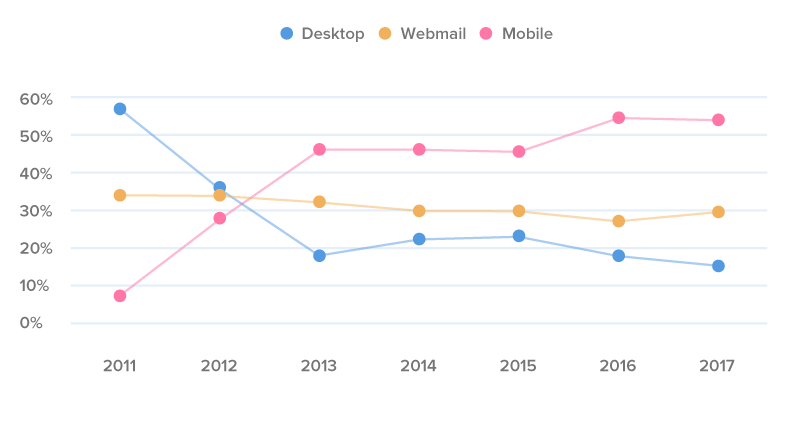
\includegraphics[width=\textwidth]{img/popularity.png}
\caption{Comparison of popularity progress of different categories of e-mail clients}
\label{fig:popularity}
\end{figure}
The popularity of the web-based and mobile clients is caused mainly by the simplicity of their deployment (no complicated configuration is usually required for their use) and the integration of many vendor-specific improvements, like search services, inter-device sharing or high availability of the service.

Despite the advantages of such interfaces, many users are forced to use less advanced solutions due to various limitations: For example, a company may choose not to submit confidential communication to its e-mail provider. Similarly, a single user may wish to process his e-mail communication locally, to avoid the issues with connectivity or provider reliability.

Such users usually deploy open-source solutions which effectively solve both the problem of vendor trust (because the software can be audited easily) and local maintainability. On the other hand, the numerous useful features (such as high-performance full-text search) and the mentioned vendor-specific improvements are typically missing in the open-source solutions.

This thesis is motivated by the concept of e-mail handling that was introduced by Google for Gmail and subsequently improved by Google Inbox. The approach completely replaces the handling of mail folders for mail organization by a more flexible use of customizable tags, and makes heavy use of Google's full-text search facilities.
Open-source solutions that would implement a decent alternative to Google Inbox are, to the best of author's knowledge, currently missing.
On the other hand, recent open-source developments have created several search engines and databases that can be used to support the underlying storage and search capabilities. Therefore, development of the alternative is possible by connecting this functionality to e-mail processing infrastructure and providing a matching modern interface for the end-user.

The goal of this thesis is to create this alternative. The specific aims include the following:
\begin{itemize}
\item high speed search for Google-like queries in large amounts of e-mails, including the tag functionality
\item integration with the e-mail processing infrastructure --- receiving, parsing, formatting and sending of e-mails
\item storing the e-mails in a reliable database
\item support for multiple users and account management
\item web-based user interface comparable to modern commercial solutions, using modern UI toolkits and frameworks to promote extensibility
\end{itemize}
The resulting open-source software package is called KamehaMail. It is possible to run KamehaMail on any modern UNIX operating system with a modern working mail server (including exim or postfix). The search functionality is provided by open-source search-engine database ElasticSearch.

This thesis is structured as follows: \Cref{mailprocess} describes the processing of e-mail messages and related Internet infrastructure. \Cref{textsearch} details the functionality of full-text search databases and their deployment in the real environments. \Cref{implementation} describes the implementation of KamehaMail, including the implementation of the backend (server part) and browser-based frontend. Performance of the resulting software is briefly benchmarked in \cref{results}. After conclusion, a short installation and user guide is provided in \cref{userguide}.

\paragraph{Related Work and Software.}
There exist a great amount of open-source web-based e-mail interfaces, such as squirrelmail, roundcube, rainloop, mailspring or notmuch-web. Most of them support full-text search using IMAP search or other own means. Yet, the handling of the e-mails as its done by Google Inbox is on whole different level on both end-user's side and the functional side. KamehaMail is trying to be as close as possible to the commercial interfaces while implementing open-source tools.

\chapter{Electronic mail processing}
\label{mailprocess}
E-mail or Electronic mail is a mean for sending and receiving messages between two users on the internet. To process an e-mail, it is necessary to understand the format of e-mail message as defined by multiple RFCs (Request for Comments). Generally, an e-mail is a text document separated into a header and a body. The header contains meta-information about the e-mail, the body contains the actual message. Encoding of the messages is further explained in the 
\autoref{mime}.

This chapter describes the important parts of the format for the processing of an e-mail message as defined by RFC 5322~\cite{rfc5322}, the protocols that define the e-mail communication (SMTP, IMAP and POP), and the transfer agents that make use of these protocols and ensure the communication.

\section{History}
First use of electronic messages as a form of communication can be traced back to early 1960s\footnote{\texttt{http://www.nethistory.info/History\%20of\%20the\%20Internet/email.html}}. Using the Compatible Time-Sharing System, hundreds of users at the MIT Computation Center could log into the remote dial-up terminals to store their files.
This way of sharing data encouraged new ways of communication to be invented. The \texttt{mail} command for the CTSS was written in the 1965 to work with e-mail within a single computer.

Ray Tomlinson is considered to be the creator of the e-mail: He was the first one to use the symbol @ for denoting a message to be sent between the computers on ARPANET in 1972. Since then, ARPANET encouraged the usage of e-mails which quickly became widespread. Soon after, the protocols and tools for the foldering and e-mail organization were invented.

Historically, one of the most important e-mail standards is \emph{Simple Message Transfer Protocol} (\emph{SMTP}), defined in the 1982. Starting as a complement to the already existing \emph{Unix to Unix Copy Program} (\emph{UUCP}), SMTP soon started to be widely used. Nowadays, majority of the e-mail communication is done via SMTP.  Nevertheless, the protocol is designed only for the message-pushing transfers. Additional protocols are required to support other use-cases.

\emph{Post Office Protocol} (shortly \emph{POP}) appeared in the 1984. It was an important standard as it stated the rules of an e-mail message retrieval to personal computers, which consequently helped to standardize the communication between the user and the mail server. Nowadays, the most used internet protocols for e-mail communication are POP3, IMAP and SMTP, further discussed in \autoref{smtp} and \autoref{popimap}.

\section{Message Format}
Multiple standards defining the e-mail message format were created throughout the years. Probably the most important one was defined by RFC 822, as it was the first protocol standardizing the e-mail message format. 20 years after being published, it was replaced by RFC 2822 in the 2005 which was later obsoleted in the 2008 by RFC 5322.
The following sections summarize the current e-mail format standard, defined by RFC 5322~\cite{rfc5322}.

E-mail message, as defined by RFC 5322, is split into two major parts, the \emph{header} and the \emph{body}.

\subsection{Header}
The \emph{header} is composed of \emph{fields} that contain meta-information about the e-mail (e.g. subject of the message, sender of the message\dots).
Field is a pair of two text values separated by a colon:
\begin{center}
\texttt{field name: field value}
\end{center}
If a line in the header begins with 7-bit ASCII character, it is a field. If a line starts with white space, the value of the field from the previous line continues on the current line, which makes multi-line fields possible. The values of the fields have to be 7-bit ASCII as well. To encode a non-ASCII value of a field, \emph{MIME} encoding is used. 

\label{mime}
\emph{MIME} is a standard that describes the encoding of non-ASCII values to 7-bit ASCII (e.g. to support multiple different charsets or structured values). To encode a string in a different charset, the following syntax is used:
\begin{center}
\texttt{=?charset?encoding?encoded text?=}
\end{center}
For example:
\begin{center}
\texttt{=?iso-8859-1?Q?=A1Hola,\_se=F1or!?=}
\end{center}
After decoding the encoded text using the provided charset and the encoding, we obtain the value \texttt{¡Hola, señor!}. A typical use of the MIME encoding is the support for different languages.

Only two header fields are mandatory for each message: \texttt{Date} and \texttt{From}. All other fields are optional, however, there are several fields that are recommended and several fields that are commonly used. Most of these fields are described in \autoref{table:fields}. 
\begin{table}[t]
\centering
\renewcommand{\arraystretch}{1.4}
\begin{tabular}{l p{20em}}
 \toprule
 Field name & Description\\
\midrule
 \texttt{Date} & Date of origination (mandatory)\\
 \texttt{From} & Address of the sender (mandatory)\\
 \texttt{Message-ID} & Recommended for the message identification\\
 \texttt{In-Reply-To} & Recommended, if the message is a reply\\
 \texttt{References} & Recommended, if the message references to other messages\\
 \texttt{Sender} & Displayed sender (optional)\\
 \texttt{Reply-To} & The address to reply (optional)\\
 \texttt{To} & Displayed recipient (optional)\\
 \texttt{Cc} & Carbon Copy, used for sending copies of e-mail to multiple users (optional)\\
 \texttt{Bcc} & Blind Carbon Copy, same as Cc except the recipients are not visible (optional)\\
 \texttt{Subject} & Subject of the message (optional)\\
 \texttt{Return-Path} & Return address (optional)\\
\bottomrule
\end{tabular}
\caption{Header fields as defined by RFC 5322.}
\label{table:fields}
\end{table}
A detail worth mentioning is that the \texttt{To} and \texttt{From} fields do not have to necessarily be the same addresses as the actual sender and recipient addresses. These fields are just informative, the real addresses are given to the SMTP for the mail delivery. SMTP is described further in \autoref{smtp}. 

An example of headers of a real e-mail message is displayed in \autoref{fig:message}.
\begin{figure}
\centering
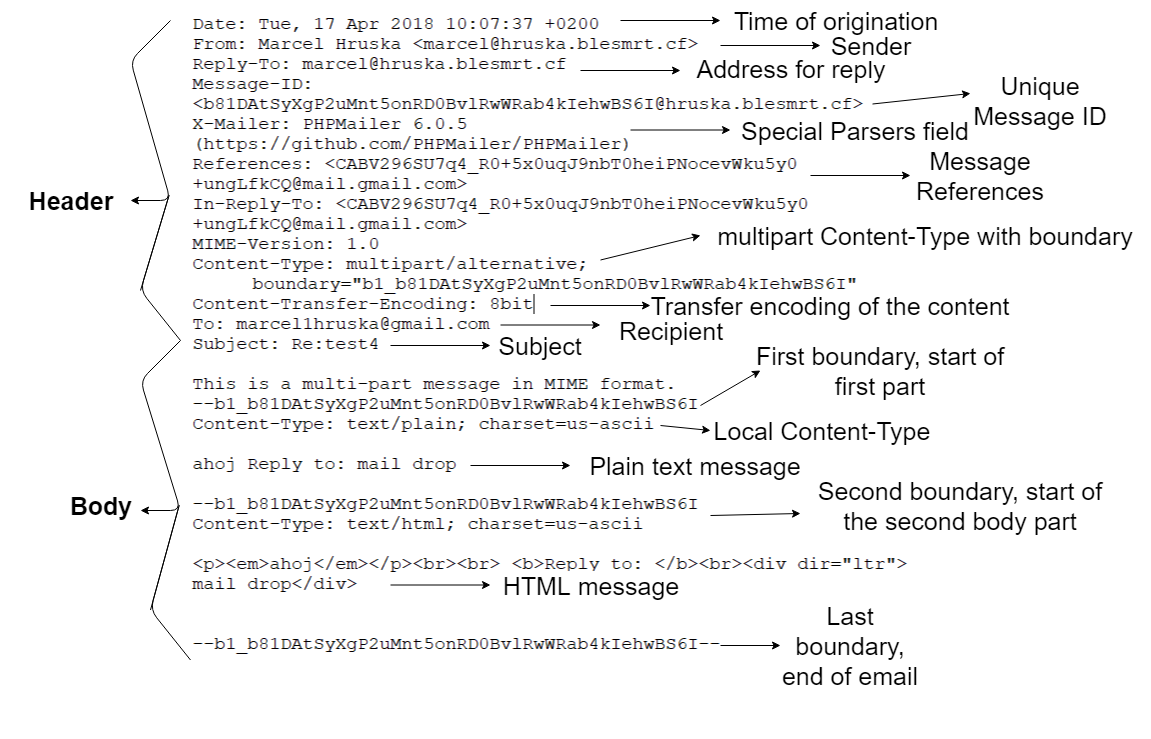
\includegraphics[width=\textwidth]{img/message_example.png}
\caption{A message sent from KamehaMail to a user of Gmail.}
\label{fig:message}
\end{figure}

\subsection{Body}
This section describes the format of the content of the message, called body.
RFC 5322 does not describe an exact format of message body, but references other documents for this purpose. For example, RFC 2045~\cite{rfc2045} from 1996 describes how the body of the message is supposed to look (its format, syntax\dots). We cover only the parts of RFC 2045 necessary for the purposes of this thesis.
The body is separated from the header by one blank line.

Originally, the messages were meant to be plain-text 7-bit ASCII only. However, it is possible to use the MIME encoding for the message bodies as well. 

If the user decides to use the MIME encoding for the message body, three header fields must be filled in: \texttt{MIME-Version}, \texttt{Content-Type} and \texttt{Content-Transfer-Encoding}.

\texttt{MIME-Version} is the version of the MIME being used for the encoding of the message, currently \texttt{1.0}.

\texttt{Content-Transfer-Encoding} specifies the encoding of the body. For example, SMTP expects messages to be 7-bit US-ASCII, which can be changed to 8-bit encoding using this header, making successive encoding more convenient.

\texttt{Content-Type} describes the type of data so that the receiving part understands how to decode the contents of the e-mail properly. This value is called \emph{media type}. Each media type has its subtype identifier, which further refines the media type. After the type identifiers comes a semicolon and parameters, if necessary. For example,
\begin{center}
\texttt{Content-type: text/plain; charset="us-ascii"}
\end{center}
defines media type \texttt{text}, its subtype \texttt{plain} and the parameter defining the charset \texttt{charset="us-ascii"}. This is also the default value, if the header is not present.

\subsubsection{Multipart messages}
There is a commonly used media type that we want to mention specifically, described by RFC 1341~\cite{rfc1341}, called \emph{multipart}.
The multipart content-type allows to combine multiple bodies/body parts in a single message, each possibly encoded in a different way. Vast majority of the modern e-mail clients uses it to send two bodies: an HTML body for the user interfaces that are capable of displaying HTML messages, and a plain-text body for the compatibility with simple plain-text interfaces.
Another widespread use of the multipart media type is to encode the attachments into the body of the e-mail.

All subtypes of the multipart content-type follow the same syntax. The header must specify a parameter called \emph{boundary}, which is used to separate the body parts by two hyphens and the boundary string. Each of the separated body parts has its own content-type header defining its inner message type. The syntax of multipart content-type is displayed in the example in \autoref{fig:message}.

\section{Message exchange}
Because it is too complicated to send a message directly to end recipient's computer with knowing only his e-mail address, a more complicated infrastructure is used for e-mail delivery. 
The computers in this infrastructure are classified by the role they have as \emph{Mail Transfer agents} (MTA), \emph{Mail User Agents} (MUA), \emph{Mail Delivery Agents} (MDA) and \emph{Mail Submission Agents} (MSA).

This section gives a closer description of the roles of e-mail agents and the communication protocols that the e-mail agents use.

\subsection{E-mail Agents}
The end-to-end delivery of a message has several stages: the submission of the message, the transfer of the message and the retrieval. Many complications can occur during the transport, such as non-existing final destination or disconnected user. \emph{E-mail agents} were invented to take care of these situations which are futher detailed in the following sections as defined by RFC 5598~\cite{rfc5598}.

\subsubsection{Mail Transfer Agent}
\emph{Mail Transfer Agent} (also known as \emph{Mail Server}) is designed to transfer e-mail messages, implementing both sending and receiving parts of the SMTP protocol.
It is often called a mail relay as well because its job is to route and forward e-mails to their final destinations.

MTAs are running in the background. They are listening to a port, waiting for the message to come, either from another MTA or from the user. If the message comes from another MTA, it is either routed to the next MTA on its path or in case that the current MTA is its final destination, stored locally for the user. 
UNIX mail servers exim, postfix or sendmail are all examples of MTAs.

MTA does not implement the access to the messages for the user, which needs to be handled by different agents.

\subsubsection{MUA, MSA, MDA}
For the communication between the user and the MTA, \emph{Mail User Agent} (also known as \emph{e-mail client}) is used. MUA 's main role is to retrieve e-mails from the MTA for the user and display them. It often implements the interface for the composition of an e-mail. E-mails created by an e-mail client are then sent to the corresponding MTA for distribution.
Usually, the communication between MUA and MTA is not direct. Two more systems are commonly used as a layer between MUA and MTA: \emph{Mail Submission Agent} and \emph{Mail Delivery Agent}.

MSA takes care of the submission of a message from MUA to MTA. It uses SMTP as well but listens to a different port. Some of the advantages of having an MSA are the following: It enforces the policies of the standard protocols while representing the interests of the author of the message. It rejects messages that do not satisfy the conditions stated by the internet standards. It includes header fields such as \texttt{Date} or \texttt{Message-ID}. In some cases, it can help to solve minor errors.

MDA takes responsibility of storing an e-mail for the user from MTA and delivers the message to the recipient's MUA. Common role of the MDA is to redirect the message to user-defined address. 

A simple diagram of the e-mail flow is shown in the \autoref{fig:mail-flow}.
 \begin{figure}
\centering
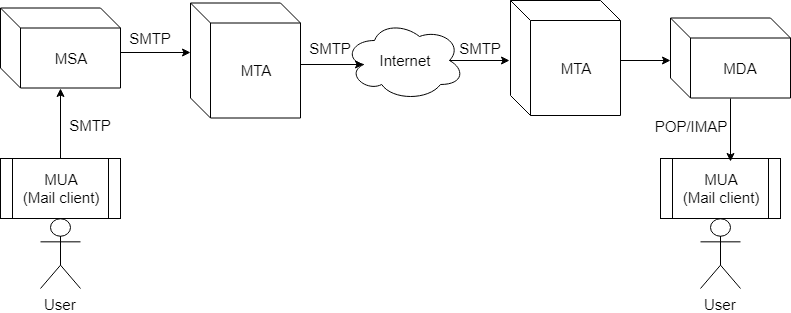
\includegraphics[width=\textwidth]{img/mail_flow.png}
\caption{A simple diagram of the e-mail transfer flow between two users.}
\label{fig:mail-flow}
\end{figure}
The transfer of the messages between two MTAs is defined by SMTP. The retrieval of the message to the MUA is done using IMAP or POP.

\subsection{E-mail protocols}
\subsubsection{SMTP}
\label{smtp}
In the previous sections, we mentioned the internet protocol SMTP which is a standard for an e-mail transfer. It was first defined in the 1982 by RFC 821~\cite{rfc821} and last updated in the 2008 by RFC 5321.
SMTP defines a model of communication as follows: The user sends a request to the sender-SMTP\footnote{sender-SMTP and receiver-SMTP are servers capable of communicating via SMTP, usually MTA} to start an e-mail communication. The sender-SMTP opens a two-way communication with the corresponding receiver-SMTP which is either an intermediate or the final destination. After that, the user can submit mail commands via the established communication path and receive the responses.
The \autoref{fig:smtp-model} shows the SMTP model as described by RFC 821.
\begin{figure}
\centering
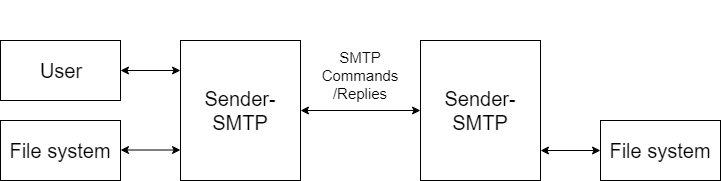
\includegraphics[width=\textwidth]{img/smtp_model.png}
\caption{Model for SMTP use.}
\label{fig:smtp-model}
\end{figure}

To begin an e-mail transaction, user introduces himself using \texttt{HELO} command. Then there are three stages of the SMTP mail transaction.
\begin{enumerate}
\item The first part is the \texttt{MAIL} command. This command indicates the beginning of a new e-mail transaction for the receiver-SMTP. The receiver-SMTP resets all the state data it has and prepares for the following commands corresponding to the new transaction.
\begin{center}
\texttt{MAIL <SP> FROM:<reverse-path> <CRLF>}
\end{center}
Tags \texttt{SP} and \texttt{CRLF} mean space and an end-of-line respectively. The \texttt{reverse-path} in the field \texttt{FROM} contains address where the responses will be sent, for example errors. If the command was processed successfully, the response \texttt{250 OK} is sent to the return address.
\item The second part is the \texttt{RCPT} command which defines the receiving address of the current mail transaction. 
\begin{center}
\texttt{RCPT <SP> FROM:<forward-path> <CRLF>}
\end{center}
The \texttt{forward-path} contains the address of the recipient. If the receiver-SMTP does not recognize the address, it responds with \texttt{550 Failure}. This command can be repeated for multiple recipients. If accepted, the \texttt{250 OK} reply is sent.
\item The third and the last part is the \texttt{DATA} command. This command transfers the actual data of the message.
\begin{center}
\texttt{DATA <CRLF>}
\end{center}
If the command is accepted by the receiver-SMTP, the reply \\ \texttt{354 Intermediate} \\ is sent. All following lines until the end of the text are the data of the message. The headers of the message are sent via \texttt{DATA} command as well.
\end{enumerate}
To end the transaction, the \texttt{QUIT} command is used.
The whole process is summarized in the following example~\cite{rfc821}:
\\
\texttt{S: HELO client.example.com}\\
\texttt{R: 250 Hello client.example.com}\\
\texttt{S: MAIL FROM:<Smith@Alpha.ARPA>}\\
\texttt{R: 250 OK}\\
\\
\texttt{S: RCPT TO:<Jones@Beta.ARPA>}\\
\texttt{R: 250 OK}\\
\\
\texttt{S: RCPT TO:<Green@Beta.ARPA>}\\
\texttt{R: 550 No such user here}\\
\\
\texttt{S: RCPT TO:<Brown@Beta.ARPA>}\\
\texttt{R: 250 OK}\\
\\
\texttt{S: DATA}\\
\texttt{R: 354 Start mail input; end with <CRLF>.<CRLF>}\\
\texttt{S: Blah blah blah...}\\
\texttt{S: ...etc. etc. etc.}\\
\texttt{S: <CRLF>.<CRLF>}\\
\texttt{R: 250 OK}\\
\texttt{S: QUIT}\\
\texttt{R: 221 Bye}\\
\label{mail-command}
There exists many other commands that SMTP protocol uses for the communication. However, this is all handled by MTA.

\subsubsection{POP and IMAP}
\label{popimap}
IMAP was defined by RFC 3501 in the 2003 and its current version is IMAP4~\cite{rfc3501}. POP was first specified by RFC 918 in the 1984 and its current version POP3 was defined by RFC 1939 in the 1996~\cite{rfc1939}. While they are both protocols designed for message retrieval for the e-mail client from mail server, POP is much older than IMAP.

The main difference between them is that IMAP is designed for multi-device use (tablet, phone, desktop\dots), displaying the same content on any device since the content is synchronized on the central server. POP is designed for downloading the e-mail from the mail server to the local machine without any synchronization. What's more, POP can be set to remove the messages from the server after download. In reality, both of the protocols can be setup to work in a very similar way. However, POP is unable to tell if the message was read or not or to provide meta-information about the existence of a folder.

Both provide advantages and disadvantages for the user. IMAP is more simple to set up for multi-device use as it does not create local storages of messages on every used device. However, usage of POP offers certain degree of privacy as the e-mails can be removed from the server after their download.

\section{End-user interfaces}
This section briefly describes end-user's phase of the e-mail transfer flow. An interface has to be provided for the user to interact with the mail server and retrieve or send e-mails. E-mail interfaces can be classified by the type of the interaction and the localization of the data.

\subsection{Desktop clients}
To proceed chronologically, the first e-mail clients described in this section are so-called \emph{desktop clients}. It is a common name for all clients that are installed on the user's machine and work with the messages locally, using the message retrieval protocols. They can be further subdivided into \emph{command-line} clients and clients with \emph{graphical user interface}.

\subsubsection{Command-line clients}
Historically, the first e-mails ever were sent using console commands. \emph{Com\-mand-line} clients provide only basic graphical interface for the user. We have already presented an example of SMTP \texttt{mail} command in the \autoref{mail-command}.
Although the command-line clients are an old technology, they are not extinct. On the contrary, they are still popular because of the safety reasons (no HTML and JavaScript), speed reasons (graphical interfaces take longer to load and respond) and the flexibility. For example, UNIX's \texttt{mail} command is still being frequently used.

\subsubsection{GUI clients}
As the displaying units grew bigger, e-mail clients with more advanced graphical user interfaces became popular. These are well-known by the average e-mail users as they are more user-friendly to use than the command-line clients. Some of the most popular e-mail clients are Mozilla Thunderbird or Microsoft Outlook. 

\subsection{Web based clients}
Another category of the e-mail clients are \emph{web based} clients or simply \emph{webmails}. The major difference between the desktop clients and the web based clients is that no e-mails are being downloaded locally to the user's computer. Instead, they are stored to the webserver and can be accessed by the user via web browser.
The first webmail was developed at CERN in 1993 by Hallam-Baker Phillip called The Mail Server Daemon~\cite{cern-mail}. Bigger development of the webmails began with the easier access to the Web in the 1990s an 2000s. 
However, using a web browser as an interface represents a certain level of threat because the communication over unsecured HTTP can be readable by third parties. Usage of encrypted HTTPS communication is highly recommended.
Some of the most popular webmail services are Gmail, Outlook.com and Yahoo! Mail and some of the most popular open-source webmails are squirrelmail, roundcube, rainloop, mailspring, notmuch-web\dots

\subsection{Mobile clients}
Currently, there is a new category, \emph{mobile} e-mail clients. Smart phones are incredibly popular and the mobile clients dominate e-mail client market share. Around 55\% of the e-mails were opened on mobile phones in the 2016\footnote{\texttt{https://litmus.com/blog/the-top-10-most-popular-email-clients-of-2016}}. They are very similar to the desktop clients, except that mobile clients are optimized for smaller touch screens.

\chapter{Text search}
\label{textsearch}
In order to create a modern, searchable e-mail interface, it is necessary to implement an algorithm that retrieves the wanted information quickly from a great amount of e-mails. The e-mail databases of some of the e-mail providers, such as Google or Outlook.com, have grown incredibly big throughout the years, containing billions of e-mails. Such databases are often far too big for naive approaches --- to find an email that contains specific keywords quickly (in milliseconds) we need a proper research of more advanced solutions for this problem.

This chapter describes the \emph{Text search}, its use in the search engines, its advantages and disadvantages comparing to the standard database search, its principles of use and implementation. 

Generally, the text search is used to find a document that contains a specific word structure in a database of text documents. In this chapter, we describe the overall process of \emph{indexing} the documents in such a database, and searching through them.

A \emph{document} is a single file of words, usually plain-text, processed and stored in the database: They are preprocessed before getting stored in order to simplify the search processing, for example by removing some unwanted (irrelevant for search) parts of the original text, such as various auxiliary words\footnote{Including e.g. articles, prepositions and conjunctions, these are usually called stop-words.} or markup, and split into so-called \emph{terms}. The terms are `clean' representations of the document content which are then stored in the database, together with the identification of the document they originated from. The list of split and processed terms associated to their documents is usually called a \emph{text-search index}. We describe this preprocessing, also usually called \emph{text analysis}, closer in \autoref{analysis}; indexing is described later in \autoref{index}.

The preprocessing of the document, as well as the searching itself, is usually done by a \emph{search engine}. A search engine is a system that integrates many text-search-related techniques to provide a coherent implementation of the indexing and querying functionality. In \autoref{engines}, we explain closer how the modern search engines work: The user requests sent to the search engine are called \emph{queries}. Each query lists some requested text words together with additional search criteria. The text in the query is processed by the same analysis that the documents are, to produce a simplified query of terms suitable for looking up in the database. The \emph{match} is the result of the search that is returned by the search engine as an answer to the given query. In other words, the match is a list of documents (in the most basic case it only contains document IDs) that
satisfy the criteria given by the query (e.g. contain the requested words).

Some search engines allow to structure the inner contents of the documents into \emph{fields}: Instead of treating all terms equivalently, users may separate them into the sets represented by the fields. A field is usually identified by string name, and contains a separately-searchable text value. For example, library databases may use fields such as \texttt{title}, \texttt{authors} or \texttt{topic}. This not only simplifies the user interface of the search, but also lowers the amount of data that need to be examined by the engine upon processing the query, because only the specific fields may be examined.

A simple diagram of the whole search cycle is provided in \autoref{fig:basic-chart}.
\begin{figure}
\centering
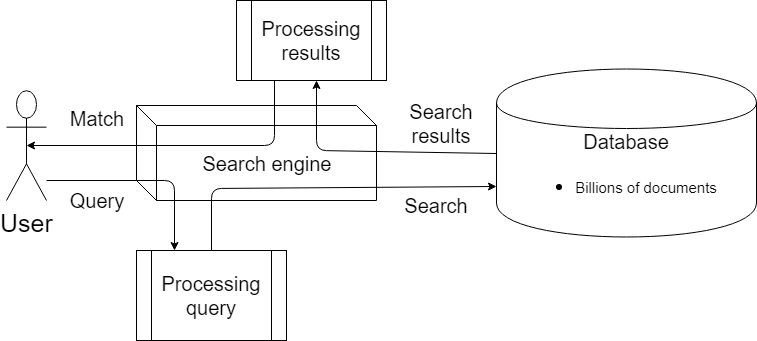
\includegraphics[width=\textwidth]{img/basic_chart.png}
\caption{A simplified view of the search cycle.}
\label{fig:basic-chart}
\end{figure}

In the following sections, we explain how the text search actually works, what processes are necessary for it to work efficiently and how to implement it.


\section{Text analysis}
\label{analysis}
There are many problems with word matching. Should  "ring" and  "Ring" match? Or  "swear" and  "swears"? In the natural human perception, we know that simply having the word at the beginning of the sentence (i.e. capitalized) does not change the meaning of the word. It is the same word as its non-capital version. We learned that "swear" and  "swears" are the same word, just in a different form. The search engine does not know that and we have to provide him with exact rules that he processes the words of the text as similarly to our perception as possible. This process is called \emph{text analysis}

Before we store the terms into the index, we need to preprocess them.
The text search analyzers are systems that process the words of the text and store them into the index. In reality, it is quite common that they treat the data in a natural way. Standard analyzers could remember the relative position, skip the insignificant words (such as "the"), treat certain fields as an exact type (e.g. date). Depending on the language, the analyzers can also decide to store the same word for its different word forms. For example, both words "forgot" and "forgotten" can be placed under the word "forget".

Generally, there are two phases of the text analysis, the \emph{tokenization} and the \emph{mapping}. \emph{Tokenization} is mandatory for creating the index but \emph{mapping} is optional and used only when needed.

The tokenization of the string is further subdivided into the following stages~\cite{elastic}.
\begin{enumerate}
\item First stage is the \emph{characters filter}. It is a preprocessing of the text before tokenization. It converts the text to the form that will be more simple to tokenize. For example, it is used to strip out HTML tags or convert \& to "add".
\item Then comes the tokenization itself. The string is split into the individual terms, accordingly to the defined analyzing parameters. The most simple tokenizers split the text whenever they encounter punctuation or whitespace, while removing the delimiter from the term.
\item The last stage is similar to the characters filter, the terms are post-processed by the \emph{tokens filter}. These filters change terms into their simplified forms, such as base forms, for easier future searching. The most common filters are lowercasing, removing the words with no possible significance to the search (stop words, e.g. "and", "the" etc.) or even adding words, such as synonyms.
\end{enumerate}

\subsection{Mapping}
As we mentioned before, there is more to the text analysis than the tokenization. We can tell the search engine how to treat specific fields and their values. For example, it is possible to have a field that contains only numbers. The search engine should understand that the value is not a simple plain string but a number. Later, it can make use of this type. For instance, the search engine can sort the results by this field. This technique is called mapping. 

Mapping is the process of defining how a document, and the fields it contains, are stored and indexed~\cite{elastic}. Which fields should be full-text fields, which should be numbers, booleans, date values, or not analyzed at all. Some search engines, for example ElasticSearch, offers the possibility to map a field using a specific language analyzer. If a field is supposed to contain only french words, the analyzer can understand the syntax of the French language and match it accordingly. For example, the word "anneau" ("ring" in English) and the word "Anneaux" have the same base form for the French language analyzer. The English language analyzer has a very little chance to understand that. Search engine remembers the specific settings for each field and processes the queries against them accordingly as well.

Different search engines use different approaches to the text analysis. How deeply is the text to be processed is mainly up to the developer that sets up the search engine.
For the purposes of this thesis, the most convenient way was to analyze almost every field. We wanted that the date of received/sent e-mail is treated as a date (milliseconds since certain date in the past) and that the results can be sorted by this value. On the other hand, there was no need to analyze fields such as \texttt{messageid} since in order to find a match, we are supposed to know the exact value. 
We did not specify any language analyzer as the users of KamehaMail can be of different nationalities, consequently writing their e-mails in different languages.

We used tokenization and mapping to process the text into terms and now we want to store them.
\section{Indexing and inverted indexes}
\label{index}
Much research has been performed to design efficient
index structures for database and information retrieval
systems~\cite{structs}. There was a need to find an ideal data structure to store and retrieve data from a database full of plain-text documents as quickly as possible. In order to do reach the solution, some sort of indexing of the split terms was needed.
A standard forward index appeared to be inefficient for the full-text search. The goal is not to look for the documents but for the words in them. Thus, the most efficient index structure is an \emph{inverted index}~\cite{invertedfiles}.

An \emph{inverted index} is structured the opposite way to the forward index. Instead of having a list of documents along with lists of terms accordingly, inverted index contains a list of terms and for each the documents that contain them. The difference between them is shown in the \autoref{table:forward-inverted}.

\begin{table}[t]
\centering
\renewcommand{\arraystretch}{1.4}
\begin{tabular}{c l}
\toprule
Inverted Index\\
\midrule
Term 1 & List of documents \\
Term 2 & List of documents \\
Term 3 & List of documents \\
Term 4 & List of documents \\
\dots & \dots \\
\bottomrule
\end{tabular}
\qquad
\begin{tabular}{c l}
\toprule
Forward Index\\
\midrule
Document 1 & List of terms \\
Document 2 & List of terms \\
Document 3 & List of terms \\
Document 4 & List of terms \\
\dots & \dots \\
\bottomrule
\end{tabular}
\caption{An inverted index (left) and a forward index (right).} 
\label{table:forward-inverted}
\end{table}

There exist two major types of inverted indexes. An \emph{inverted file} (or \emph{document-level index}) and a \emph{full inverted index} (or \emph{term-level index}). The difference is that inverted file is used only for accessing the documents of the corresponding term. It is sufficient when no other information than document's ID is needed. A full inverted index has complete information about the term in the file (e.g. position) which makes it far bigger and harder to maintain, however indispensable in certain use cases, for example, when the word position is needed.

An inverted index consists of two main parts.
\begin{enumerate}
\item The first part is the \emph{vocabulary}. It is a list of all distinct terms of all documents. Each of them can contain information about document count and about their \emph{inverted lists}. The inverted lists are associated to their respective terms directly, as a list or by a pointer to the corresponding part. The position of a word is stored as well, if it is not the document-level index. This list is ordered.
\item The second part is an \emph{inverted list} which is a list of all documents where the word appeared. These lists can be represented as pairs \((d, f_{d,t})\) where \(d\) represents the identifier of the document and  \(f_{d,t}\) is the associated set of frequencies of the term \(t\) in the document \(d\)~\cite{invertedfiles}.
This list is ordered as well.
\end{enumerate}

A simple database of documents is provided in the \autoref{table:data-ex} for the presentation purposes. Each document in the table is uniquely identified by its \texttt{ID} field. The actual text of the quote is stored in the \texttt{Text} field. The \texttt{Author} field contains the author of the quote. As we mentioned before, the terms are processed and stored to the index structure which is shown in \autoref{table:invlist-ex}. Notice that the inverted index provided in the example is made only of the field \texttt{Text}.

\begin{table}[t]
\centering
\renewcommand{\arraystretch}{1.4}
\begin{tabular}{c p{20em} l}
\toprule
ID & Text & Author\\
\midrule
1 & Your time will come. You will face the same Evil, and you will defeat it. & Arwen \\
2 & The Ring has awoken, it has heard its masters call. & Gandalf \\
3 & We swears, to serve the master of the Precious. We will swear on\dots on the Precious! & Gollum \\
4 & You shall not pass! & Gandalf \\
\bottomrule
\end{tabular}
\caption{A simple database of quotes from Lord of the Rings.} 
\label{table:data-ex}
\end{table}

\begin{table}[t]
\renewcommand{\arraystretch}{1.4}
\resizebox{\textwidth}{!}{
 \begin{tabular}{c c} 
 \toprule
 term \(t\) & \((d, f_{d,t})\) \\ 
 \midrule
 and & (1, 1) \\
 awoken & (2, 1) \\
 call & (2, 1) \\
 come & (1, 1) \\
 defeat & (1, 1) \\
 evil & (1, 1) \\
 face & (2, 1) \\
 has & (2, 2) \\
 heard & (2, 1) \\
 it & (1, 1),  (2, 1) \\
 its & (2, 1) \\
\bottomrule
\end{tabular}
\quad
 \begin{tabular}{c c} 
 \toprule
 term \(t\) & \((d, f_{d,t})\) \\ 
 \midrule
 master & (3, 1) \\
 masters & (2, 1) \\
 not & (4, 1) \\
 of & (3, 1) \\
 on & (3, 2) \\ 
 pass & (4, 1) \\
 precious & (3, 2) \\
 ring & (2, 1) \\
 same & (1, 1) \\
 serve & (3, 1) \\
 shall & (4, 1) \\
\bottomrule
\end{tabular}
\quad
 \begin{tabular}{c c} 
 \toprule
 term \(t\) & \((d, f_{d,t})\) \\ 
 \midrule
 swear & (3, 1) \\
 swears & (3, 1) \\
 the & (1, 1),  (2, 1),  (3, 3) \\
 time & (1, 1) \\
 to & (3, 1) \\
 we & (3, 2) \\
 will & (1, 3),  (3, 1) \\
 you & (1, 2), (4, 1) \\
 your & (1, 1) \\
 & \\
 & \\
\bottomrule
\end{tabular}
}
\caption{A document-level inverted index for the database shown in the \autoref{table:data-ex} with only word occurrences.}
\label{table:invlist-ex}
\end{table}

Nowadays, there are plenty of variations for the inverted index structure. Several possibilities were mentioned in the article written by Mahapatra and Biswas~\cite{invindex}. For instance, some of them store meta data. Apart from the additional information stored for each word (such as the frequency of the occurrence or the word position), these implementations contain meta-information about each hit. \emph{Hit} is an exact word position in the document. These meta data may contain information such as font type, font size, text type etc\dots Other solutions mentioned in the article implement both types of the inverted indexes, the full inverted index and the inverted file, each for different situations.

Creating an inverted index is a simple task. However, it can be challenging to create it without wasting memory and CPU. Advancements in the hardware do not provide any significant help because the collections are growing in size even faster. An efficient way is needed for creating, storing and maintaining the index.

\subsection{Construction of inverted index}
The fastest and the most simple way to construct an inverted index is to build the whole collection in memory. However, this approach is not possible for bigger collection (i.e. billions of documents, terabytes of data). Such collections do not fit in the memory and disk has to be used which is always costly. An optimized method that
creates small, memory fittable inverted lists, stores them to disk and merges them when all is done is needed. Moffat and Bell or Heinz and Zobel described several methods solving this problem~\cite{invindex}.

\subsection{Structure of the inverted index}
The article written in 1996~\cite{structs} defines two following approaches for the inverted index structures.

The first approach is to maintain an inverted index only for the document access. Specifically, only document IDs are returned upon a matching query. A postprocessing is needed to retrieve additional information about the document, if wanted. That is done by using a term-level index. This approach has a significant disadvantage, as the number of the matching documents can be large, the postprocessing can be time consuming. Although, it can be improved by using an internal tree representation.

The second approach is about having an index for each element type. It may create a huge space overhead as each term must appear in every index. There were attempts for removing the duplicates, for example by using a combined vocabulary. Nevertheless, the space overhead was still far too great.
Many different possible structures exist which take care of the duplicates and improve the consequential space overhead.

To further reduce space consumption, compressions can be applied on the inverted lists~\cite{invindex}. For example, instead of storing all the numbers as 32-bit integers, variable-length numbers can be used.

\subsection{Segmentation}
The maintenance of already existing inverted index also causes an issue. Inserting a new element into a sorted list and updating the whole index with possibly billions of documents directly is too expensive.

ElasticSearch uses the principles of \emph{segmentation} as defined by Lucene and the following facts will be interpreted as explained in the guide for ElasticSearch~\cite{elastic}. 

Instead of rewriting the whole inverted index again upon each new entry, completely new indexes are created with the recent results. Such supplementary index is called a \emph{segment}. Lucene describes the index as a collection of segments and a commit point. Commit point serves as a common entry point for its segments, the query is performed against it, the commit point then distributes the query to all its segments and returns the results combined.
The \autoref{fig:commit} shows an example of the segmentation.
\begin{figure}
\centering
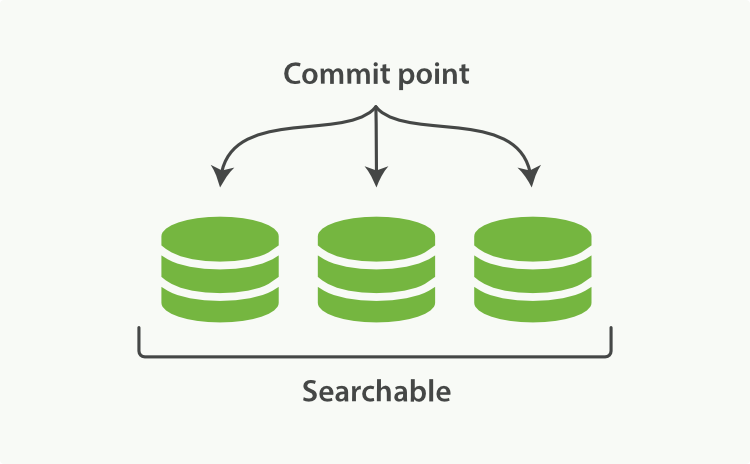
\includegraphics[width=.8\textwidth]{img/commit.png}
\caption{A commit point for three segments of the index.}
\label{fig:commit}
\end{figure}
This may cause an issue because the approach may create an enormous amount of small segments which consume additional CPU and memory, rendering inverted indexes inefficient.
It can be at least partially improved by merging the segments, transparently for the incoming search query and the user. It is most convenient to run this process when a new, not yet committed (not yet written to the specific commit point) segment has been set. Currently committed segments are taken along with the new uncommitted one and merged. The new merged segment is then committed into the commit point and the old ones are to be removed. To remove them safely, the search engine must be sure that there are no searches being performed on them which usually delays their removal.

The problems mentioned above are not the only problems concerning inverted indexes. However, they are efficiently solved by the search engine we integrated to the application, ElasticSearch. The specifications of ElasticSearch are mentioned in \autoref{es}. 

\section{Query structure}
\label{query}
Once the database is constructed and prepared for the text search queries, it is possible to search in it. Search engines usually provide an API to make the communication with them (i.e. send the queries and receive the match data) possible. The following examples are written in a JSON-based syntax, similar to the ElasticSearch~\cite{elastic} but simplified for presentation purposes. The queries are effectively performed against the inverted index to the database shown in \autoref{table:data-ex}. The \texttt{Text} field part of the database is displayed in \autoref{table:invlist-ex}.

A simple query looking for the term "ring" is shown in the following example:
\begin{code}
{ "query": { 
    "term" : "ring"
} }
\end{code}
The second document contains term "ring" and it is the only match. The most basic result to the above query returns only the matched documents' IDs:
\begin{code}
{ "hits": [
    { "ID" : 2 } ] 
}
\end{code}
\texttt{Hits} is an array of results. For each matching document, it contains at least the document's ID. Nonetheless, there are cases where we want to have more information about the document than its ID. For example, other contents of the matching documents or the relevancy of the document to the given query.

Queries can be more complex, defining different logical search criteria. We can use logical NOT (for the unwanted terms), AND (for multiple terms) and OR (for optional matches). In the following example, user is looking for those documents that contain terms "master" and "precious", cannot contain term "ring" and optionally may contain term "evil":
\newpage
\begin{code}
{ "query" : { 
     "bool" : {
       "must" : {
        "term" : "precious",
        "term" : "master"
      },  "must_not" : {
        "term" : "ring"
      },  "should" : {
        "term" : "evil"
      }
} } }
\end{code}
The first document contains the term "evil" but it does not have any of the obligatory terms, so it will not be a match. The document 4 does not contain any of obligatory terms. The document 2 neither and furthermore it contains the forbidden term "ring". The document 3 contains both of the obligatory terms, does not contain term  "ring" which makes it the only match. It is still a match even if it does not have the term "evil" which was meant to be optional.

In the previous examples, the search field was not specified so the search engine looked at all fields. If we want to find all of the Gandal's quotes, we can write the following query:
\begin{code}
{ "query": { 
    "term" : "gandalf"
} }
\end{code}
This is a legit query that returns documents 2 and 4 as results. But it searches through all the fields, \texttt{Text} and \texttt{Author}. This may be time consuming. Depending on the length of the Gandalf's quotes and the amount of his quotes in the database, such queries can be inefficient. 
To save time, we specify the field in the following example:
\begin{code}
{ "query": { 
    "term" : {
        "Author" : "gandalf"
} } }
\end{code}
Let's say that this time we want that the search engine returns more information about the matching document, for example the text of the quote:
 \begin{code}
{ "hits": [ { 
      "ID" : 2,
      "_source" : {
        "Text"  : "the ring has awoken it has heard its
                        masters call" 
      } }, { 
      "ID" : 4,
      "_source" : {
        "Text"  : "you shall not pass" 
} } ] }
\end{code}

\paragraph{Search details description.}
The full-text search does not look for a simple key but rather for content~\cite{invertedfiles}. When the user provides a query, he is looking for the meaning inside the text according to it. The search engine should evaluate the query not only in a lexical way but also in a contextual way. In order to ensure this behaviour, the search engine needs exact rules for ranking the results appropriately. First of all, it uses the very same analyzer for the query as it used for the documents stored in the database.
This method ensures that upon looking at a specific word, we will get its other word forms as well. In certain implementations even synonyms.

Typical steps for the query evaluation are the following~\cite{elastic}. 
\begin{enumerate}
\item First, the type of the field in the query is checked, to determine if it should be analyzed or not.
\item If necessary, the query string is analyzed using the according analyzer.
\item Then, the search engine looks into the inverted index and finds the IDs of the matching documents.
\item Using the matching document IDs, the search engine can provide, if requested, various additional information, such as relevance of the match or values of other fields of the matching documents.
\end{enumerate}

In case that query fails and does not find any matching documents or the match does not evaluate as expected, the user can decide to refine the query in various ways. We already mentioned that the full-text search tries to find the most relevant results and sort them that way. The following sections details the ranking of the match.

\subsection{Relevance and effectiveness}
There is an issue of the quantification of the relevance. Is it possible to measure the relevance of a term in the document?
Relevance of word to the text can be considered subjective or inexact. The document can be relevant to the given query even though it contains none of the terms~\cite{invertedfiles}.

Because of this inexact attribute of the relevance, the attribute \emph{effectiveness}~\cite{invertedfiles} is preferred. The engine is considered to be effective if the number of the matched results is as close as possible to the expected results.
Effectiveness is typically described by two aspects, \emph{precision} and \emph{recall}. Recall measures the quality of the results, it is a fraction between the matches found and all the relevant matches. Precision measures the quantity of the results, it is a fraction between the relevant matches found and all matches found.
 
We want to know how to measure the relevance. The number indicating the relevance of a document to the given query is called the \emph{score}. In the following example, the score will be a number between zero and one. One means the result is as relevant as possible. Zero means the result is completely irrelevant and will not be displayed at all.
There are multiple ways to evaluate the score of the match~\cite{elastic}: the occurrences of the query in the document or the format of the term. Recall that some implementations of the inverted indexes contain meta data of the original text. In that case, it is simple to check if the querying term was a header or bold before the text analysis. Another method is to compute how big portion of the text the term takes. The following example searches for word "you" in \autoref{table:invlist-ex} and sorts the matches by the relevance of the term "you" in the matched documents:

 \begin{code}
{ "hits": [ { 
      "_id" : 1,
      "_score" : 36.5
    },
    { 
      "_id" : 4,
      "_score" : 23.5
} ] }
\end{code}

Two documents matched. For presentation purposes, we create a simple version of pseudo-procedure for evaluating the score of the match:
\begin{enumerate}
\item For each exact occurrence of the term, add 10 points to the score. Add 3 extra points for each capital letter in the occurrence.
\item For each similar occurrence of the term, add 5 points to the score (can be adjusted depending how similar the occurrence is). Add 1 extra point for each capital letter in the occurrence.
\item Add 0.5 point for each percent of the text the occurrence takes. If the occurrence takes generally 30\% of the text, add 15 points. (This can be normalized to the whole length of the text. The bigger the text, the less likely the term will be relevant).
\end{enumerate}
According to this algorithm, the document 1 has 2 * 10 points for the exact occurrences and 3 extra points for the capital letter, 5 points for a similar occurrence ("your") and 1 extra point because it starts with the capital letter again. Finally, "you" takes together almost 15\% of the whole quote, which means another 7.5 points are added, resulting in 36.5 points together for document 1.

The document 4 gets only 10 points for one occurrence and 3 points because it has a capital letter. The term takes roughly 21\% of the quote which means another 10.5 points are added, resulting in 23.5 points together for document 4.

This simple algorithm determined that term "you" is more relevant in the quote "Your time will come. You will face the same Evil, and you will defeat it" than in the quote "You shall not pass!".

The real implementation of the scoring algorithms can be far more complex, taking in consideration the length of the field or the inverse document frequency~\cite{elastic}. The ElasticSearch uses own formula which is mentioned \autoref{es}.

\subsection{Phrase query}
The user does not only searches for one term. The vast majority of the web search queries contain phrases, multiple words in a single query field. For the database search, it is an easy task to perform a phrase query --- if the document contains the phrase as it is, match it. The text search takes in consideration the relevance and it needs a way to measure the relevance of the phrase query as well. The user expects that the most relevant results should be those documents that contain the phrase as a whole. The more words in the phrase query are separated from each other in the document, the less relevant it should be. 

Three possible procedures were mentioned in the article written by Zobel and Moffat~\cite{invertedfiles}.

The first procedure is that the phrase is indexed as a term and that it has its own inverted list. This solution is often too space consuming, as it is impossible to predict which two-word pair phrases are necessary to be stored. Creating all possible two-word pairs creates an absurdly big collection (three-word, four-word\dots). It can be improved by partial indexing and combinations.

Another way is to simply split the phrase and run a separate query for each split term. This may possibly return seemingly irrelevant matches, as the words can happen to be anywhere in the document, have no actual meaning together and still be a well-ranked match.

Last mentioned procedure is to keep the word positions in the index so that the position of the phrase can be determined during evaluation.

These three procedures can cooperate together and the final implementation of the phrase query evaluation is possibly a combination of them. However pure use of only one of them will not return reasonable results.

The users of KamehaMail will very likely use phrase querying which is again handled by ElasticSearch.

We described all necessary things to understand the steps needed for a working search engine. In the following part, we look at the search engines themselves, compare them to the standard database search and provide some statistics about them.

\section{Search engines}
\label{engines}

\subsection{Comparison with relational indexing methods}
Search engines are similar to the database systems~\cite{invertedfiles}. The documents are indexed and stored in the database, the search engine evaluates the queries against the index and finds the match. However, there are differences mostly in the way the queries are performed and the way the documents are stored. For instance, the majority of the queries for the search engines are just lists of terms while the database systems are facing complex queries (SQL). On the other hand, the database systems are matching only specific logical condition, the search engines take in consideration the relevance of the document to the given query. Consequently, the database search returns all matches while the search engines return fixed number of matches, sorted by the score of relevance. Returning all matches would not be possible in certain cases because the result of the query may be huge (millions of documents).
That is because the resulting documents may contain terms that are at least in some minimal way similar to the query but almost completely irrelevant for the user.

\subsubsection{Advantages}
The main advantage of the text search comparing to the standard database search is in the way they process the words of the text.

Standard database search with its binary query cannot even partially understand the context of the text. It cannot make use of the index when looking for similarity. For example, if we want to find all Gandalf's quotes with possible suffixes (\texttt{WHERE Author LIKE Gandalf\%}), the standard database se\-arch does not use the index, it has to look at every row and check if it is a match. In many cases, that is an unwanted and insufficient behaviour. This also makes the standard database search slower, as it is not optimized for similarity searching.

We already know that text search understands the value of the data, refers to it as it was written in human language and behaves that way~\cite{elastic}. Many of the search engines are capable of matching synonyms or understanding the context. When we are looking for the phrase "Fox News", we actually do not want news about foxes but some news published by Fox News. Many distinct approaches of data evaluation can be defined to the specific fields by the developer. 

\subsubsection{Disadvantages}
There are few disadvantages to the text searching when comparing with the standard database search.

An index for a text search can be massively bigger than a standard B-Tree index. B-Tree is a self-balancing tree structure for searching, inserting and deleting in logarithmic time. A full text search index (or inverted index) contains duplicates, which can potentially make it several times bigger.

Another disadvantage is hard maintainability of the inverted indexes. The fact that the lists of documents are sorted and potentially large makes it difficult to insert into them in a reasonable time. However, there exist improvements as well.
 
\subsection{Web search engines}
Text searches most essential use is in the web search engines. They index the webpages and so provide an easier access to information that was inconceivable a few decades ago~\cite{invertedfiles}. Several of the following facts were published in the article written by Lawrence Page and Sergey Brin~\cite{google}.
They stated that developing a Web Search engine is a difficult task, as it has to process tons of web pages along with tons of search queries. The Web is rapidly growing every day, with more and more webpages being created. In the 1994, one of the first web search engines, the World Wide Web Worm had an index of 110,000 web pages. In the end of 1997, WebCrawler claimed to have from 2 million to 100 million documents. In the present, the biggest and the top search engine is Google. On the 12th of January, it stated that it had more than 47 billions of webpages indexed~\cite{wwwstats}, as we can see in \autoref{fig:graph_googleweb}. 
\begin{figure}
\centering
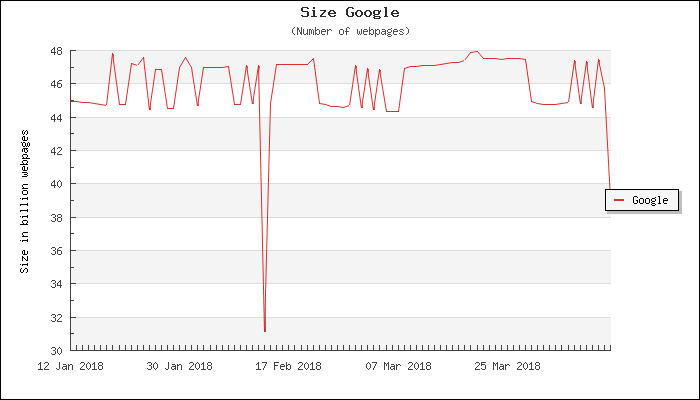
\includegraphics[width=.8\textwidth]{img/google_webpages.png}
\caption{The amount of webpages indexed by Google}
\label{fig:graph_googleweb}
\end{figure}
Google proved to be the most used web search engine by processesing the vast majority of all the web search queries. It held 81.53\% of the search engines market share from January 2017 to January 2018, as shown in \autoref{fig:graph_market}\footnote{provided by \texttt{netmarket.com}}.
\begin{figure}
\centering
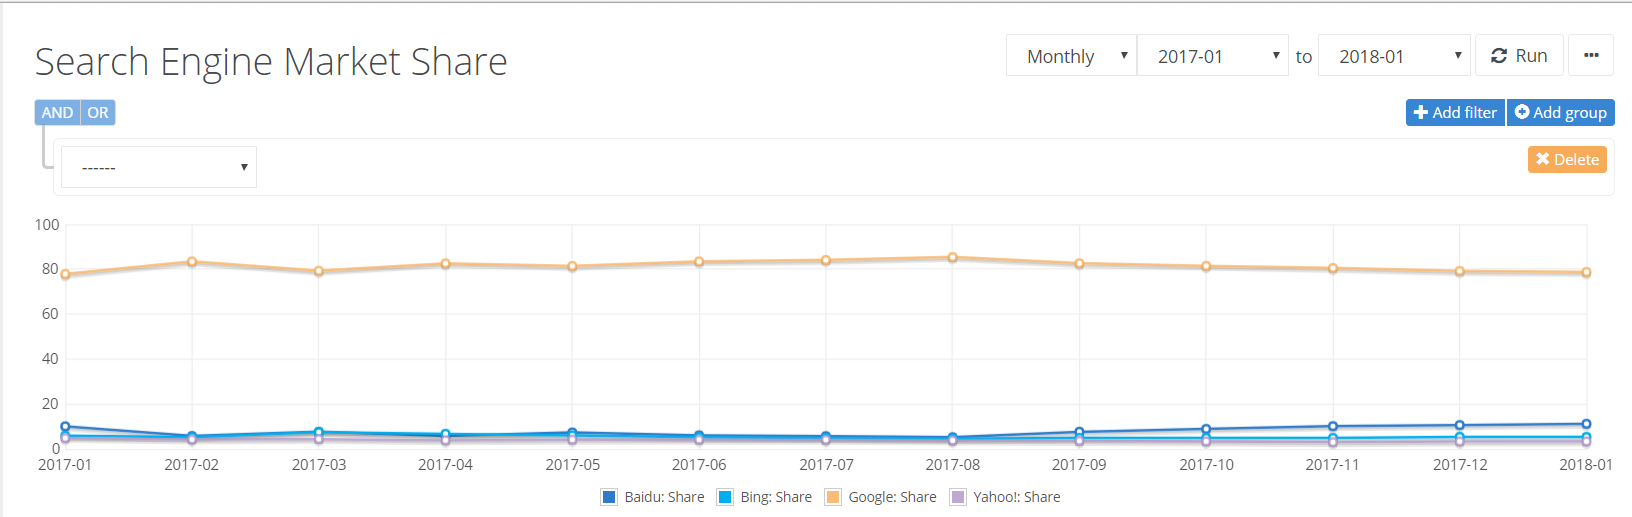
\includegraphics[width=.8\textwidth]{img/search_engine_market.png}
\caption{The search engine market on all platforms in 2017.}
\label{fig:graph_market}
\end{figure}

Complementary to the already mentioned automated search engines relying on keyword matching, there exist human maintained search engines. They may return more sufficient answers but are expensive to build and hard to maintain~\cite{google}.

The collections used by the search engines can be vastly distinct from each other: For example, they can vary in size. Some collections can be as small as tens of megabytes and grow each day by only few hundreds of documents. Others may contain tens of gigabytes (e.g. libraries) but still grow slowly. Web collections are different, they are not only extremely huge, but the amount of indexed data can change drastically both ways. Google has currently around 40 billion documents indexed. However, on the 17th of February, they had indexed only around 31 billions of documents.

The search engine we found to be the most attractive option for KamehaMail is ElasticSearch. As we covered the topic of text search and the search engines, we can look into its specifications.

\subsection{ElasticSearch}
\label{es}
In this part, we detail the specific implementation parts of the ElasticSearch because we integrated it into KamehaMail for the role of search-engine database. All the facts and information are interpreted from the book written by Gormley and Tong~\cite{elastic}.
ElasticSearch is very popular open-source analytics and search engine built on top of Apache Lucene, which is a full-text search library, used by corporations such as Wikipedia or Github. ElasticSearch runs on its own server communicating via provided RESTful API and JSON.

In the following paragraphs, we cover most of the implementation problems that we faced earlier in this chapter and look at the solutions ElasticSearch provides.

\subsubsection{Document Metadata}
ElasticSearch has three mandatory meta data fields stored along with the document. \emph{Index} is a document collection where the document is stored. \emph{Type} is a subcategory of the index. It defines specific mappings to the documents of the same type. This mapping is stored with the type and the queries performed against it are analyzed the same way. It is possible to have several types in the same index.
The last field is \emph{id} which is a string that along with the index and type uniquely identifies the document.

\subsubsection{Structure}
ElasticSearch uses a specific terminology for its structures. The main part of whole system is a \emph{cluster}. A \emph{Cluster} is a collection of servers that are capable of indexing, searching and holding all the data. These servers are called \emph{nodes}. It is possible to run multiple nodes in a single cluster. An image of empty initialized cluster is shown in \autoref{fig:empty-cluster}. It is a one node cluster, called \texttt{master}.
\begin{figure}
\centering
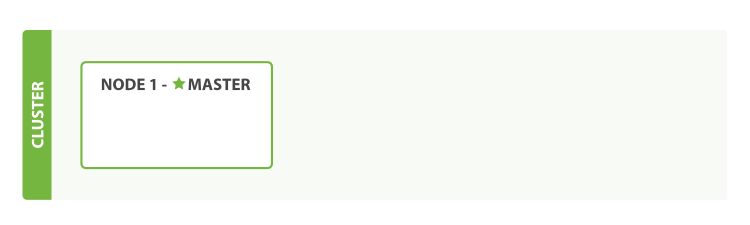
\includegraphics[width=.8\textwidth]{img/empty_cluster.png}
\caption{An empty cluster.}
\label{fig:empty-cluster}
\end{figure}

We would like to remind the problem of large amount of the data in an index mentioned in \autoref{index}. ElasticSearch solves this by splitting the index into the user-defined amount of \emph{shards}. \emph{Shard} is an independent and fully-functional index, capable of searching and indexing by its own.
The usage of shards is fully transparent to the user. In addition, ElasticSearch provides a possibility of creating copies of the shards, called \emph{replicas}. \emph{Replicas} are 1:1 clones of shards, used to ensure high availability of the indexed data. If new data is inserted into the primary shard, it is copied to its replica as well.
The replicas are also used to speed up the search by working concurrently with the shards.
An example of simple commonly used cluster is shown in \autoref{fig:replicas} that contains three shards and one replica for each shard.
\begin{figure}
\centering
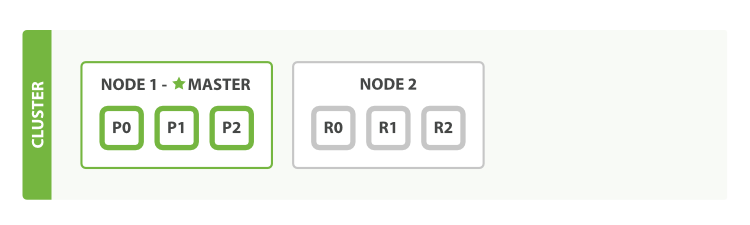
\includegraphics[width=.8\textwidth]{img/replicas.png}
\caption{A cluster with one node Master that is subdivided into three shards P0, P1 and P2. In the node 2, there is one replica shard (R0, R1, R2) for each primary shard.}
\label{fig:replicas}
\end{figure}

\subsubsection{Result score}
ElasticSearch uses \emph{Lucene's practical scoring function}~\cite{elastic} for ranking the matches.
The formula is as follows:
\begin{align*}
\centering
\textrm{s}(q,d) = \textrm{nq}(q) \cdot \textrm{c}(q,d) \cdot \sum_{t \in q}\textrm{f}(t,d) \cdot \textrm{if}(t)^2 \cdot\textrm{b}(t) \cdot \textrm{nt}(t,d),
\end{align*}
where
\begin{itemize}
\item $s(q,d)$ is the final relevance score of the query $q$ in the document $d$,
\item $\textrm{nq}(q)$ is the query normalization factor, it is used for normalizing the query $q$ in order to be able to compare it to the others,
\item $\textrm{c}(q,d)$ is the coordination factor, used to add additional score to the documents that contain higher percentage of the query terms,
\item $\textrm{f}(t,d)$ is the frequency of the term $t$ in the document $d$,
\item $\textrm{if}(t)$ is the frequency of the term $t$ in the inverted index,
\item $\textrm{b}(t)$ is a boost to the term $t$ for the query $q$, and
\item $\textrm{nt}(t,d)$ is the field-length normalization. The shorter the field, the higher the weight.
\end{itemize}

We believe that ElasticSearch is a great choice for performing the full-text search in the database of indexed e-mails as it is provides strong performance and simple interface.

\section{Application to mail indexing}
Short response time for searching in e-mails is necessary for modern e-mail user interface. 
To provide this feature, we parse the information from an e-mail message and index it into the respective fields of ElasticSearch's index. The analyzed fields are \texttt{subject}, \texttt{text}, \texttt{to} and \texttt{from}. Non-analyzed fields are \texttt{messageid}, \texttt{references} and \texttt{tag} as we want an exact match and not similarity match. The last used field is \texttt{date} which is not only analyzed but also mapped (by standard date formats) because we want the results to be sorted primarily by the date and then ranked by the relevance.

Not only user-defined searches but also many other functions are handled by ElasticSearch. Grouping of the emails by references is done by ElasticSearch. As the e-mail directory-based hierarchy is replaced by tags, these are searched by ElasticSearch as well.

\chapter{Implementation}
\label{implementation}
In this chapter, we show an overview of all the implementation tools and procedures that we used to create KamehaMail. The implementation is separated into two major parts: the backend which communicates with the mailserver and the search engine, and the browser-based frontend that provides an interface to the end-user. These two parts communicate with each other using API calls.

\section{Backend}
 The implementation of the backend follows the usual style of deployment of PHP application. The software on the server is organized as follows:
\begin{itemize}
\item \emph{Apache HTTP server} is used to serve the static frontend files and the end-user's web browser, and provides the translation of the browser-originated HTTP API calls to the PHP application.
\item The application is run by \emph{PHP} with several additional modules (the complete list is shown in \autoref{userguide}).
\item The application communicates with \emph{Exim4} mail server using standard UNIX methods: \texttt{sendmail} for sending e-mail and pipe-based transport for receiving. Exim handles the communication with the e-mail infrastructure using standard internet protocols. It is also possible to integrate other mail servers.
\item \emph{ElasticSearch} is installed for searching and indexing the e-mails. The server communicates with it via REST API using \texttt{curl} requests.
\end{itemize}

\subsection{Data storage}
The data on the server are stored on two different places: the primary storage of the e-mails as files in user directories, and the secondary indexed storage in ElasticSearch.

The primary storage is organized as follows: in a specified directory 
the application stores the meta-information about users
(e.g. login details) and the users' mailboxes.

The mailbox section contains all the stored e-mails. Each e-mail is uniquely identified by its 64-character Sha-256 hash. The e-mails are separated into users' subdirectories, in which they are further separated into a subdirectory structure based on first few characters of the hash, to minimize the problems with large directories.

The meta-information section contains two SQLite databases, \texttt{usersdb} and \texttt{loginkeys}. \texttt{usersdb} is a list of all users and their corresponding passwords. \texttt{loginkeys} is a list of the currently logged users and their corresponding login API keys (further explained in \autoref{userapi}).

The directory hierarchy is displayed in \autoref{fig:folder-tree}.
 \begin{figure}
\centering
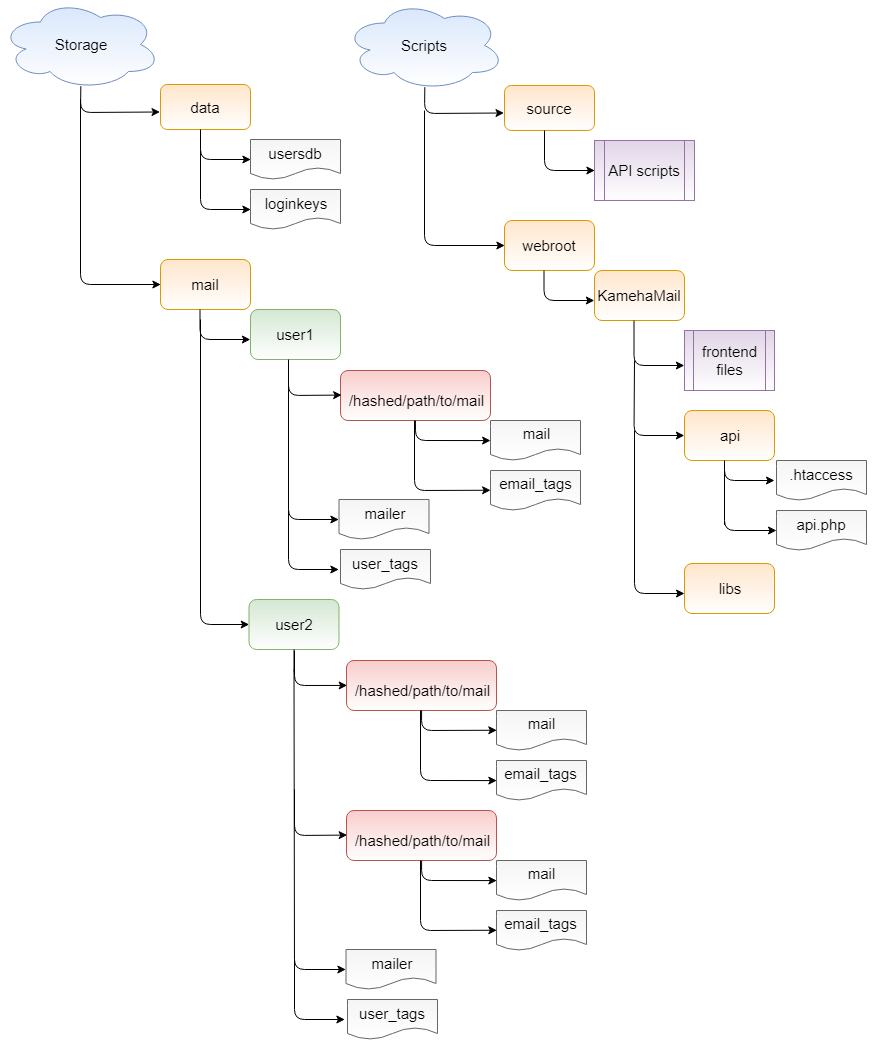
\includegraphics[width=\textwidth]{img/folder_tree.png}
\caption{A folder hierarchy on the server}
\label{fig:folder-tree}
\end{figure}

\subsection{API}
All of the server side scripting was done in PHP. To simplify the communication between the frontend and the backend, we created a set of API calls which run specific PHP scripts.

To provide REST-like API calls, htaccess is used. If an HTTP request is directed to the folder where the \texttt{.htaccess} is located, \texttt{htaccess} takes the request's URL and forwards it as a query string to a beforehand defined script. For example, upon calling URL
\begin{center}
\texttt{hruska.blesmrt.cf/KamehaMail/api/some-work}
\end{center}
htaccess takes a part of the url after its folder's name (i.e. \texttt{some-work}) and sends it to the \texttt{api.php} as a query string. \texttt{api.php} serves as a relay or a router. It loads all necessary source scripts and calls other PHP scripts accordingly to the received query string.

We provide an example of the processing of the user login API request:
\begin{enumerate}
\item  A HTTP POST request is sent from the frontend to the URL\\\texttt{api/client/login} with the data: \texttt{username} and \texttt{password}.
\item \texttt{.htaccess} in the api folder processes the url string and redirects\\\texttt{client/login} as a query string to the \texttt{api.php}.
\item \texttt{api.php} parses the query string, calls an external \texttt{login} function (defined by \texttt{login.php} in the source folder) with the username and password as parametres.
\item The login function checks the credentials and returns a JSON formatted response whether the login was successful or not, together with a new API key (which is simultaneously stored to the \texttt{loginkeys} database).
\item Then \texttt{api.php} forwards the response to the frontend.
\end{enumerate}

The source folder contains many of the PHP scripts for different uses. In the \autoref{fig:folder-tree}, they are denoted as \texttt{API scripts}. Depending on their purpose, they can be divided into three categories:

\subsubsection{Client calls}
\emph{Client} scripts are used for the account management such as logging or changing passwords.
\begin{itemize}
\item \texttt{login.php} validates the given credentials. In case of success, it creates a loginkey (hash of the current time, username and password), saves it to the \texttt{loginkeys} database and sends it to the frontend which saves it to the browser as well (similar to cache). This loginkey is later used to validate the API calls.
\item \texttt{checklogged.php} checks whether the currently saved loginkey is valid. If yes, logged user is redirected to his e-mails page.
\item \texttt{logout.php} removes the currently used loginkey from the database and redirects the user to the homepage.
\item \texttt{mailer.php} contains functions for setting/getting the mailer of the user.
\item \texttt{password.php} changes the password of the user.
\item \texttt{signup.php} creates new user entry in the \texttt{usersdb} database and a new folder in mail. It also initializes new index in the ElasticSearch with the user's name and the e-mail mapping.
\item \texttt{usertags.php} contains functions for adjusting the user's tags. Each user can have self-defined tags which are stored in their mail folder.
\label{userapi}
\end{itemize}

\subsubsection{Integration of the ElasticSearch to the server}
\emph{Elastic} scripts communicate with the ElasticSearch via provided RESTful API. We implemented it to the API scripts using PHP curl requests.  
The following code is an example of a PHP \texttt{curl} request which calls Elastic's search API.
\pagebreak
\begin{code}
$req = curl_init();
    
curl_setopt_array($req, [
    CURLOPT_URL            =>
	 "http://localhost:9200/user/email/_search?pretty",
    CURLOPT_CUSTOMREQUEST  => "GET",
    CURLOPT_POSTFIELDS     => $data,
    CURLOPT_HTTPHEADER     => [ "Content-Type: application/json" ],
    CURLOPT_RETURNTRANSFER => true,
]);
    
$response = json_decode(curl_exec($req));	
$curl_close($req);
\end{code}
\texttt{\$req} is an initialized \texttt{curl} request. \texttt{CURLOPT\_URL} ultimately contains the API call. The call is directed to the localhost:9200\footnote{ElasticSearch listens to this port} with index \texttt{user}, type \texttt{email} and the function \texttt{\_search}. \texttt{\$data} contains the query in a JSON format. The response is sent as a JSON string back from ElasticSearch and saved in \texttt{\$response}.
We implemented following scripts which use ElasticSearch:
\begin{itemize}
\item \texttt{search.php} processes user's query and reformats it to the ElasticSearch's syntax. After being processed by ElasticSearch, the results of the search are sorted by the \texttt{date} field. \texttt{search.php} in fact runs two searches. The first search finds e-mails relevant to the given query and returns their identifiers. Second search creates so-called mail groups:  The e-mails are grouped by references to create a conversation-like interface. ElasticSearch's search is called for each matched document, matching also the documents which have the already found identifier in their references. This will result in a list of grouped e-mail identifiers where in each group at least one of the e-mails was a result of the former user's query.
\item \texttt{updatetags.php} changes tags in ElasticSearch for the specific e-mail.
\item \texttt{removeMail.php} removes the e-mail from ElasticSearch.
\item \texttt{saveMail.php} puts new e-mail document to the ElasticSearch. If the inserted e-mail has some references (to already present e-mails), each of the referenced e-mail messages is updated with its \texttt{message-id}.
\item \texttt{reindex.php} takes hashes of already stored e-mail in the database and gives their parsed content to ElasticSearch for reindexing.
\end{itemize}
 
\subsubsection{Communication with e-mail server and processing of e-mails}
\emph{E-mail} scripts implement the handling of e-mails:
\begin{itemize}
\item \texttt{maildrop.php} is called when the mail server receives new message. It retrieves its content and forwards it to the \texttt{decide} function (defined by \texttt{decide.php}).
\item \texttt{decide.php} is the actual brain behind storing the messages. It checks whether the recipient is a legit address, parses the contents of the message, creates tags, stores it to the mail directory and forwards the parsed data to the saving function of ElasticSearch.
\item \texttt{downloadAtt.php} temporarily saves the received attachment to the server and forces the browser to download it. Then removes the attachment.
\item \texttt{getMail.php} receives resulting IDs from Elastic's \texttt{search} function and processes them. It finds the corresponding e-mail files in the mail directory, parses them and sends their contents to the frontend which displays them. It also takes care of the date separation of the e-mails.
\item \texttt{changetags.php} changes user's tags.
\item \texttt{removeAtts.php} contains function which is called whenever the upload of the attachments was cancelled or the e-mail was sent, to remove them from the server.
\item \texttt{removeMail.php} removes the e-mail from the mail directory.
\item \texttt{saveMail.php} saves the e-mail to the mail directory.
\item \texttt{sendMail.php} creates headers for sending an e-mail and sends it.
\item \texttt{upload.php} temporarily uploads the attachments to the server, for future sending.
\end{itemize}
We used two external libraries to simplify the processing of e-mail text: \emph{mailparser}\footnote{\texttt{https://github.com/php-mime-mail-parser/php-mime-mail-parser}}, which extracts headers, bodies and attachements from an e-mail, and \emph{PHPMailer}\footnote{\texttt{https://github.com/PHPMailer/PHPMailer}}, which creates all necessary headers for sending a message and actually sends it.

The source folder also contains an administration interface, which is accessible using \texttt{admin.php}. The usage of admin interface is further described in \autoref{userguide}.

\section{Frontend}
Frontend provides the interactive visual side that come to contact with the user. The frontend is coded in JavaScript, HTML and CSS.

\paragraph{Choice of JavaScript framework.}
Framework is a software structure that provides functionality for building specific applications. Some of the most favourite JavaScript frameworks are Vue, Angular, React or Ember. We chose \emph{Vue}\footnote{https://vuejs.org/} for KamehaMail because it is fast, scales well and has a simple API to use.
Its core part is a Vue instance which configures the application, binds the data and attaches the application to a specific DOM element. Another important thing is that there exists a component framework for Vue, called \emph{Vuetify}\footnote{https://vuetifyjs.com/en/}. It is a UI toolkit, providing many templates that are directly cooperating with Vue.
We used several of these templates to make KamehaMail pleasant to look at.

\paragraph{Frontend application structure.}
The frontend is divided into three important parts. Each of them consists of an HTML file and a JavaScript file. The first part is \texttt{index}, which is the first thing an user will encounter upon opening the main site. It is a simple login menu with an option to sign up. On successful login, user is redirected to the main menu where he can see his e-mails.
The second part is \texttt{signup} which is visually very similar to the \texttt{index}. The third and the biggest part is \texttt{emails} which implements all of the interface's features.
For the message text editor we integrated \emph{quill}\footnote{consists of two parts, official quill from \texttt{https://quilljs.com/} and the Vue implementation for it taken from \texttt{https://github.com/surmon-china/vue-quill-editor}}.All used libraries, such as Vue, Vuetify and jQuery are stored along with their CSS files in the folder \texttt{libs} in KamehaMail, to be accessible to the frontend.

\subsection{Communication with the server}
The frontend and the backend communicate with each other via asynchronous POST HTTP requests sent from the frontend to the server. The frontend uses the jQuery's feature \texttt{ajax}, which takes care of sending the requests and receiving the responses from them in a user-friendly way.

\chapter{Results}
\label{results}
In this chapter, we investigate the performance of the resulting software.

KamehaMail is fully functional and implements almost all of the intended features. Additionally, we test the scalability of the searching capabilities of the interface on large amount of e-mails.

\section{Benchmark setup}
First of all, we prepared an environment sufficient for testing. Enron e-mail data set\cite{klimt2004enron} is a collection of roughly half million e-mails, freely accessible for anyone. Using the implemented admin interface, we dropped and indexed the Enron e-mails into one mailbox in the database. The e-mails were tagged according to the original position in the folder.

We measured the results on two data sets of different sizes to provide better overview of performance scaling.

The first data set consists of almost 27.000 e-mails found in the mailbox of the Enron user V. Kaminski. The second data set consists of 200.000 e-mails selected randomly from multiple mailboxes. The full data set was not benchmarked because of resource limitations.

On both data sets, we measured the space needed for their storing in the database, and the time required to complete several testing queries.

\section{Benchmark results}
The results obtained on the indexed data sets are reported in \autoref{table:bench}.

As expected, the more complicated cases were tested, the longer it took ElasticSearch to give the results. Increases in response time were caused by more complex queries, more indexed e-mails and more returned results. On the other hand, from the perspective of the user, the 7.4-times increase in the amount of data did not have a significant impact on the response time of the search. 

The indexing process itself scaled satisfactorily --- indexing performance was approximately 40 e-mails per second on average, and it varied only negligibly with the increase of the index e-mail count.
\begin{table}[t]
\centering
\renewcommand{\arraystretch}{1.4}
\begin{tabular}{p{10em} l l}
 \toprule
Query & 26.675 e-mails & 200.000 e-mails\\
\midrule
\texttt{tag:inbox} & &\\
\hline
Top 10 results & 1ms & 5ms\\
Top 50 results & 3ms & 8ms\\
Top 100 results & 8ms & 11ms\\
\hline
\texttt{tag:inbox and approval}  & &\\
\hline
Top 10 results & 14ms & 48ms\\
Top 50 results & 16ms & 68ms\\
Top 100 results & -- & 70ms\\
\hline
\texttt{tag:inbox and approval and time:<1.1.2002}  & &\\
\hline
Top 10 results & 18ms & 52ms\\
Top 50 results & 20ms & 59ms\\
Top 100 results & -- & 57ms\\
\hline
 & &\\
\hline
E-mail files disk space & 417MB & 2.7GB\\
ElasticSearch's index disk space & 112MB & 394MB\\
\bottomrule
\end{tabular}
\caption{Search and space results from benchmark performed on Enron e-mail data set.}
\label{table:bench}
\end{table}

\chapter*{Conclusion}
\addcontentsline{toc}{chapter}{Conclusion}
This thesis has reviewed the necessary means and tools for creating a modern, web-based end-user e-mail interface, mainly the high-performance full-text search and customisable tags, while avoiding the usage of mail folders for mail organization. The main result of the thesis, the mail interface KamehaMail, provides a simple open-source alternative to the commercial user interfaces (e.g. Google Inbox).

In \autoref{mailprocess} we have discussed the format of e-mail messages, e-mail exchange on the Internet and several details of the related e-mail infrastructure; including the classification of mail-transfer agents and brief description of the used communication protocols. We reviewed and classified some of the existing end-user e-mail interfaces, which are the main concern of this thesis.

In \autoref{textsearch}, we have described the currently used techniques for creating a working searchable database using an inverted index structures, which can be later used for implementing a database capable of high-performance. We have provided several examples of used queries and of the matching process. At the end, the chapter compares the full-text search to standard database search and looks briefly at the current search engines.

Finally we have connected an open-source search engine ElasticSearch to the mail processing infrastructure and a web-based end-user interface to create KamehaMail. Implementation details, used tools, frameworks and libraries are detailed in \autoref{implementation}. 

We have benchmarked KamehaMail (and ElasticSearch) by indexing approximately 200 thousand e-mails from the publicly available Enron e-mail data set~\cite{klimt2004enron} and measuring the search time required to complete several queries in the resulting mailbox. The results are available in \autoref{results}.

KamehaMail can run on any reasonably modern UNIX-like operating system that can run a mail server, a web server, and ElasticSearch. A simple installation and user guide is provided in \autoref{userguide}.

\section{Future work}
The implementation of KamehaMail is not perfect and we provide ideas for the improvement of both interface and the API library:
\begin{itemize}
\item Implement safety measures against JavaScript e-mail messages.
\item Support for more complex queries. The search possibilities of the current interface are limited due to the desired simplicity of the user queries. ElasticSearch offers great variety of different options for querying, which can be mapped to the syntax of KamehaMail queries to expose more functionality to the users.
\item Implementation of built-in calendar and a snooze feature (known from Google Inbox) would benefit the connection of user e-mail management to time-management. KamehaMail API can be easily extended to support this feature.
\item Hierarchical tags are a feature that can provide the hierarchical mail-classification workflow of nested directory structures while still providing the ability to search by tags without the cumbersome parallel maintenance of both classification structures. ElasticSearch supports this kind of tagging via wildcard queries.
\item Addition of more user account management possibilities, e.g. avatars, signatures, mail aliases, addressbooks, or other commonly expectable features.
\item Improve the design of the interface to work nicely on smartphones (or generally smaller screens), or create a native mobile application that communicates directly with the KamehaMail API.
\item Caching of the search results to the browser for speeding the interface's response time.
\end{itemize} 

%%% Bibliography
%%% Bibliography (literature used as a source)
%%%
%%% We employ bibTeX to construct the bibliography. It processes
%%% citations in the text (e.g., the \cite{...} macro) and looks up
%%% relevant entries in the bibliography.bib file.
%%%
%%% The \bibliographystyle command selects, which style will be used
%%% for references from the text. The argument in curly brackets is
%%% the name of the corresponding style file (*.bst). Both styles
%%% mentioned in this template are included in LaTeX distributions.

\bibliographystyle{alpha}    %% Author (year)
% \bibliographystyle{unsrt}     %% [number]

\renewcommand{\bibname}{Bibliography}

%%% Generate the bibliography. Beware that if you cited no works,
%%% the empty list will be omitted completely.

\bibliography{refs}

%%% If case you prefer to write the bibliography manually (without bibTeX),
%%% you can use the following. Please follow the ISO 690 standard and
%%% citation conventions of your field of research.

% \begin{thebibliography}{99}
%
% \bibitem{lamport94}
%   {\sc Lamport,} Leslie.
%   \emph{\LaTeX: A Document Preparation System}.
%   2nd edition.
%   Massachusetts: Addison Wesley, 1994.
%   ISBN 0-201-52983-1.
%
% \end{thebibliography}


\appendix
\chapter{User Guide}
\label{userguide}
In this appendix, we provide a user guide for running the interface on own infrastructure or simply using it for e-mail management.

The appendix is separated into two sections. The first section describes the interaction with the interface on the end user's level. The second section details the API library, and explains how to run the interface on a UNIX server.

\section{Interface interaction}
KamehaMail can be tried on the webpage \texttt{hruska.blesmrt.cf/KamehaMail} using any reasonable modern web browser. The main page is a simple login panel with sign up option. To registrate, go to the \texttt{Sign Up} option, choose a username (with domain at the end, in this case \texttt{@hruska.blesmrt.cf}).

After successful login, the e-mails page shows up. There are several points of interest:

\paragraph{Left navigation panel.}
Left navigation panel contains tags for e-mails. First four tags are system tags, \texttt{Inbox}, \texttt{Archive}, \texttt{Trash} and \texttt{Sent}. After them comes menu with customisable user-defined tags\footnote{list of possible icons for tags can be found on \texttt{https://material.io/tools/icons/}}. There is a possibility to create a search tag from the current search.

\paragraph{Top bar.}
The top bar contains search panel (center) and account management menu (right). Possible queries for the search are the following:
\begin{itemize}
\item User can simply type the term he is searching for. In this case, the search engine will look into all analyzed fields for the match.
\item User can specify the search field, for example \texttt{subject: Hello}. Possible search fields are \texttt{subject}, \texttt{text}, \texttt{from} and \texttt{to}
\item There is one more unanalyzed search field named \texttt{tag}. Any system or user-defined tags can be searched using the same syntax (e.g \texttt{tag: inbox}).
\item User can filter the results by date. Date value must be in \texttt{time: dd/mm/yyyy} or \texttt{time: dd.mm.yyyy} format. Possibilities of date filtering are:
\begin{itemize}
\item lesser than \texttt{time: <date}
\item greater than \texttt{time: >date}
\item between \texttt{time: date-date}
\item exact date \texttt{time: date}.
\end{itemize}
\end{itemize}
All of the queries above can be combined using \texttt{and}, creating multi-criteria queries with any number of white spaces in between.
Account management provides options for password change, mailer change and logout.

\paragraph{Center.}
The button in the bottom right corner opens a form for writing a new e-mail. It features text editor and a file drop for attachments.

The center contains grouped e-mails. Each group indicates the number of the e-mails it references to and the subject of the conversation. If the subject is in bold, one or more messages in the conversation are new (i.e. unread). The tag buttons are to the right of the subject: mark read/unread, archive, delete and a drop-down menu for user's tags.
Preview of each e-mail is shown once the group is opened. Each e-mail group provides text editor and \texttt{Quick Reply} option to reply directly to the conversation. Reply and forward options on the right side of each e-mail open a new prefilled form for sending.

All basic features are displayed in \autoref{fig:menu}.
\begin{figure}
\centering
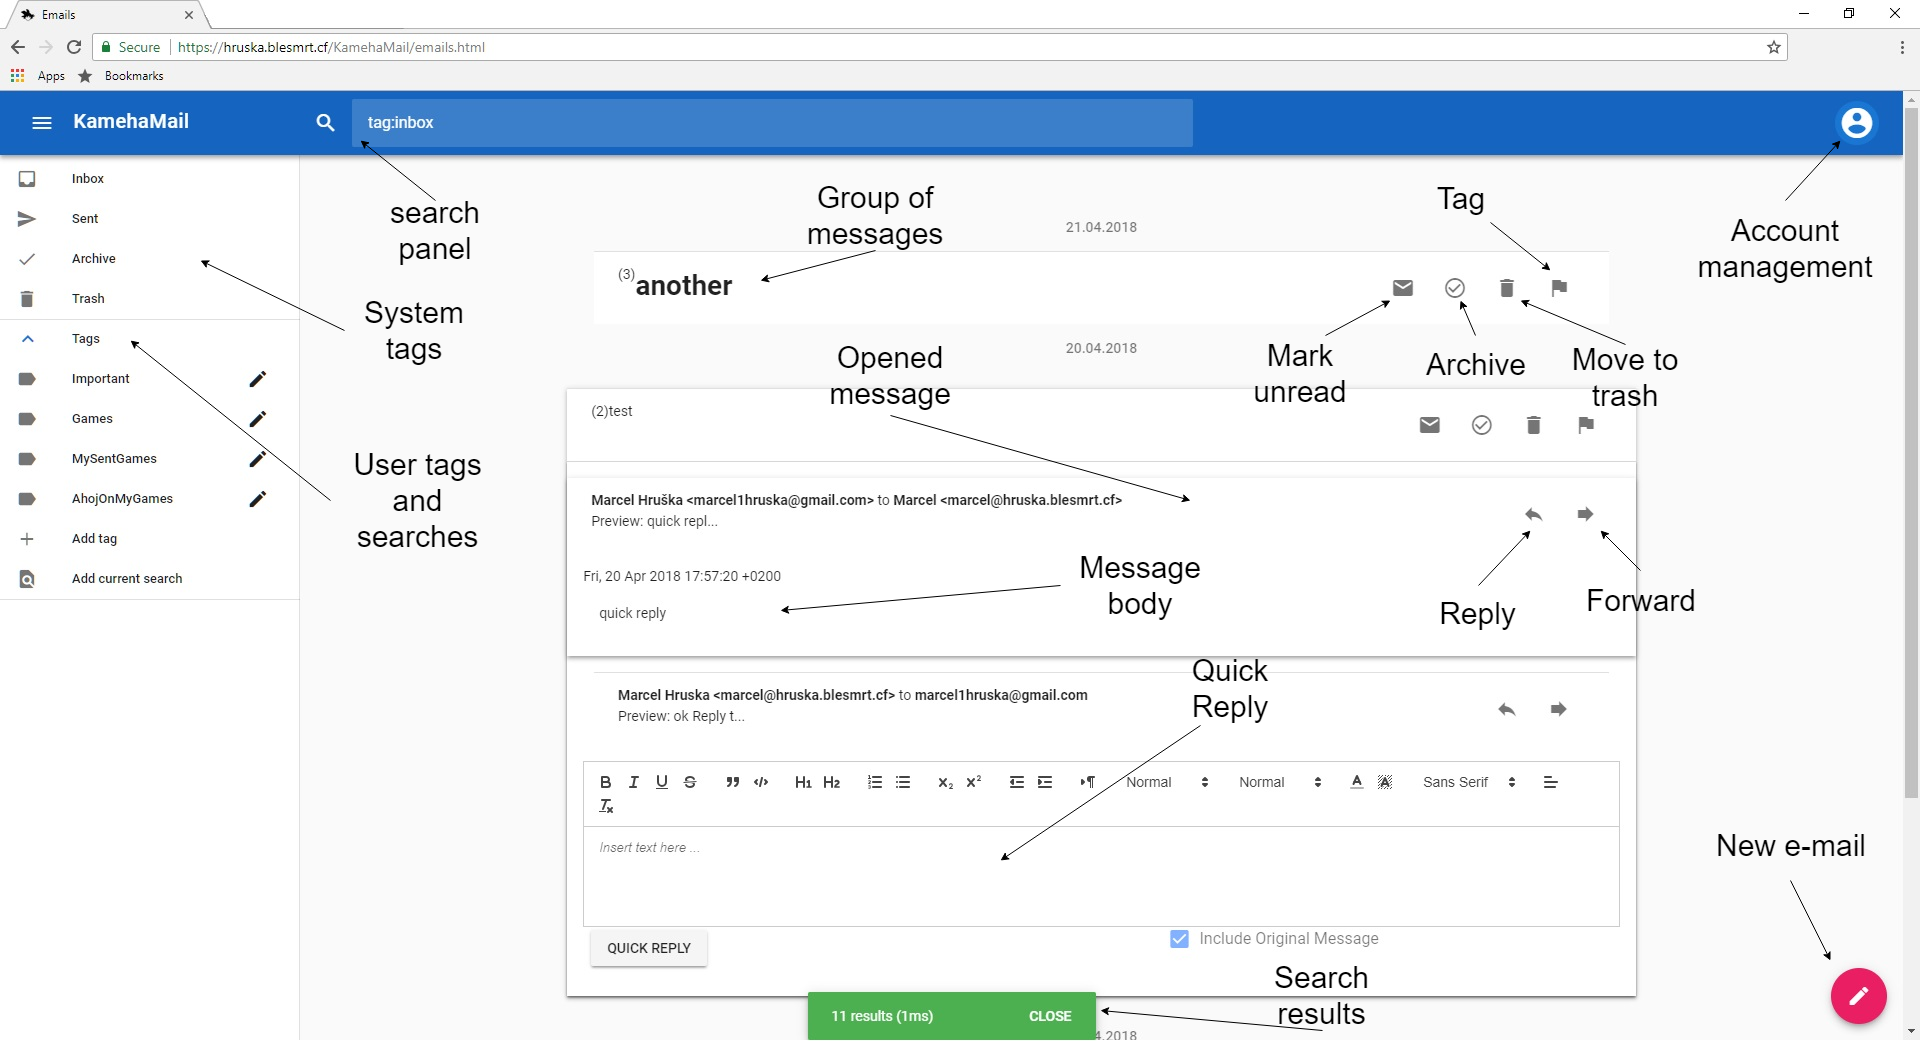
\includegraphics[width=\textwidth]{img/menu.png}
\caption{Main menu description.}
\label{fig:menu}
\end{figure}

\section{Server configuration}

We briefly cover the installation procedure for getting KamehaMail working on a UNIX server. The requirements are:
\begin{itemize}
\item A running ElasticSearch cluster accessible on \texttt{localhost} port 9200.
\item A web server (Apache is preferred because of the \texttt{.htaccess} usage, but any webserver capable of request rewriting will work). Apache module \texttt{mod\_rewrite} is required; \texttt{mod\_ssl} is highly recommended since KamehaMail does not do any encryption of data on its own. Using \texttt{mod\_suexec} for executing the API is also recommended for additonal security.
\item A working mail server (we use Exim4 as an example, but any server that can route local mail delivery to a program pipe will work, including Postfix, Sendmail, Courier and other).
\item PHP interpreter, preferably of version 7 or better, with following modules available:
\begin{itemize}
\item php-curl
\item php-gd
\item php-json
\item php-mail
\item php-mailparse
\item php-mbstring
\item php-net-smtp
\item php-net-socket
\item php-pear
\item php-sqlite3
\item php-xml
\end{itemize}
\end{itemize}



For the installation, KamehaMail backend is extracted on the server. The source code can be currently obtained from the Git repository at \url{https://github.com/hrusticka123/KamehaMail}.

The configuration consists of creating a storage space for the primary e-mail database, configuring Apache webserver and setting up the local mail transport to KamehaMail.

\begin{enumerate}
\item Paths to mailbox directory, data directory (as described in \autoref{implementation}) are filled into \texttt{source/config.php}, together with the full absolute path to the \texttt{source} directory. KamehaMail script should have write access to the mailbox and data directory. \texttt{/var/lib/kamehamail} is a preferable location for both.
\item The extracted directory contains a subdirectory \texttt{webroot}, which is where Apache document root should be directed. Webroot contains a subdirectory \texttt{api} with files \texttt{.htaccess} and \texttt{api.php}, which serve as a gateway to the rest of the implementation. Apache must be configured to execute \texttt{api.php} as a CGI script (possibly by FastCGI, FCGID or php-fpm).
\item Path to the \texttt{source} directory must be filled in \texttt{api.php} so that it can find the rest of the backend source code.
\item To allow mail exchange, the UNIX user that runs KamehaMail source code must have access to \texttt{sendmail} command.
\item Receiving mail from the mail server is implemented by piping the incoming e-mail to the script \texttt{maildrop.sh}, which forwards it to the PHP application. Configuration of Exim4 for this behavior consists of several steps that modify the Exim4 configuration:
\begin{enumerate}
\item The mail domains that are handled by KamehaMail instance are put into the list \texttt{dc\_other\_hostnames}, which effectively makes them `local domains' for Exim.
\item The local user transport is changed to\\ \texttt{transport = transport\_kamehamail}.
\item A corresponding transport configuration is created in the directory with mail transports:
\begin{code}
transport_kamehamail:
	driver = pipe
	command = /var/www/example.org/maildrop.sh
	user = kamehamail-user
	group = kamehamail-group
\end{code}
(Path to \texttt{maildrop.sh}, user and group should be changed to match local setup.)
\end{enumerate}
Other mail servers can be set up for similar behavior.
\end{enumerate}

After setting up and reloading all services, KamehaMail should be ready to register new users and accept e-mail.

Extra interface is provided for the usual administrative commands: script \texttt{source/admin.php} can be run with \texttt{php} to execute administrative tasks, such as user management, reindexing or e-mail injection. The list of commands is available in \autoref{table:admin-calls}. For example, a new user is added by running:\\
\texttt{php api.php add\_user john.doe@example.com johnspassword} \\
The same interface was used during benchmarking to easily index the dataset and make it available to the web interface for measurements.
\begin{table}[t]
\centering
\renewcommand{\arraystretch}{1.4}
\begin{tabular}{p{6em} l l p{6em}}
 \toprule
Description & Command & Parameters & Script standard input \\
\midrule
Inject \mbox{an e-mail} & \texttt{drop} & \texttt{user@domain tag} & RFC-formatted content of e-mail\\
Reindex mail &  \texttt{reindex} & \texttt{user@domain} & list of hashes to reindex\\
Add user & \texttt{add\_user} & \texttt{user@domain password} & -- \\
Remove user & \texttt{remove\_user} & \texttt{user@domain} & -- \\
Remove \mbox{a specific} mail & \texttt{remove\_mail} & \texttt{user@domain} & list of hashes to remove\\
\bottomrule
\end{tabular}
\caption{Administration interface command listing.}
\label{table:admin-calls}
\end{table}


\openright
\end{document}



E-mail je v dnešnej dobe nenahraditeľným komunikačným prostriedkom na Internete. Jedny z najpopulárnejších rozhraní na prácu s e-mailami sú webové rozhrania, kedže sa jednoducho spúšťajú a integrujú viaceré, pre dodávateľa špecifické vylepšenia, ako sú napríklad služby na vyhľadávanie. Napriek týmto výhodám viacerí používatelia využívajú menej pokrokové riešenia, kvôli možnosti spravovať svoje e-maily na vlastnej infraštruktúre. 

Táto práca má za cieľ vytvoriť voľne dostupnú alternatívu ku komerčným užívateľským rozhraniam, inšpirovanú Google Inbox-om, implementovaním moderných voľne dostupných nástrojov a knižníc. Vo všeobecnosti na vytvorenie e-mailového rozhrania musíme najprv naštudovať formát e-mailovej správy a spôsob komunikácie pomocou e-mailov. Kvôli podpore vysokorýchlostných plnotextových vyhľadávaní, táto práca taktiež opisuje techniky a štruktúry používané v plnotextovom vyhľadávaní, aby sme mohli implementovať príslušný prehľadávací nástroj a databázu do infraštruktúry na spracovanie e-mailov. Navrch toho je poskytnuté webové rozhranie pre užívateľa pre spravovanie e-mailov, ktoré spája vyššie spomenuté funkcionality.
}

% 3 to 5 keywords (recommended), each enclosed in curly braces
\def\Keywords{%
{key} {words}
electronic mail, full-text search, databases
}

%% The hyperref package for clickable links in PDF and also for storing
%% metadata to PDF (including the table of contents).
%% Most settings are pre-set by the pdfx package.
\hypersetup{unicode}
\hypersetup{breaklinks=true}

% Definitions of macros (see description inside)
%%% This file contains definitions of various useful macros and environments %%%
%%% Please add more macros here instead of cluttering other files with them. %%%

%%% Minor tweaks of style

% These macros employ a little dirty trick to convince LaTeX to typeset
% chapter headings sanely, without lots of empty space above them.
% Feel free to ignore.
\makeatletter
\def\@makechapterhead#1{
  {\parindent \z@ \raggedright \normalfont
   \Huge\bfseries \thechapter. #1
   \par\nobreak
   \vskip 20\p@
}}
\def\@makeschapterhead#1{
  {\parindent \z@ \raggedright \normalfont
   \Huge\bfseries #1
   \par\nobreak
   \vskip 20\p@
}}
\makeatother

% This macro defines a chapter, which is not numbered, but is included
% in the table of contents.
\def\chapwithtoc#1{
\chapter*{#1}
\addcontentsline{toc}{chapter}{#1}
}

% Draw black "slugs" whenever a line overflows, so that we can spot it easily.
\overfullrule=1mm

%%% Macros for definitions, theorems, claims, examples, ... (requires amsthm package)

\theoremstyle{plain}
\newtheorem{thm}{Theorem}
\newtheorem{lemma}[thm]{Lemma}
\newtheorem{claim}[thm]{Claim}

\theoremstyle{plain}
\newtheorem{defn}{Definition}

\theoremstyle{remark}
\newtheorem*{cor}{Corollary}
\newtheorem*{rem}{Remark}
\newtheorem*{example}{Example}

%%% An environment for proofs

%%% FIXME %%% \newenvironment{proof}{
%%% FIXME %%%   \par\medskip\noindent
%%% FIXME %%%   \textit{Proof}.
%%% FIXME %%% }{
%%% FIXME %%% \newline
%%% FIXME %%% \rightline{$\square$}  % or \SquareCastShadowBottomRight from bbding package
%%% FIXME %%% }

%%% An environment for typesetting of program code and input/output
%%% of programs. (Requires the fancyvrb package -- fancy verbatim.)

\DefineVerbatimEnvironment{code}{Verbatim}{fontsize=\small, frame=single}

%%% The field of all real and natural numbers
\newcommand{\R}{\mathbb{R}}
\newcommand{\N}{\mathbb{N}}

%%% Useful operators for statistics and probability
\DeclareMathOperator{\pr}{\textsf{P}}
\DeclareMathOperator{\E}{\textsf{E}\,}
\DeclareMathOperator{\var}{\textrm{var}}
\DeclareMathOperator{\sd}{\textrm{sd}}

%%% Transposition of a vector/matrix
\newcommand{\T}[1]{#1^\top}

%%% Various math goodies
\newcommand{\goto}{\rightarrow}
\newcommand{\gotop}{\stackrel{P}{\longrightarrow}}
\newcommand{\maon}[1]{o(n^{#1})}
\newcommand{\abs}[1]{\left|{#1}\right|}
\newcommand{\dint}{\int_0^\tau\!\!\int_0^\tau}
\newcommand{\isqr}[1]{\frac{1}{\sqrt{#1}}}

%%% Various table goodies
\newcommand{\pulrad}[1]{\raisebox{1.5ex}[0pt]{#1}}
\newcommand{\mc}[1]{\multicolumn{1}{c}{#1}}


% Title page and various mandatory informational pages
\begin{document}
%%% Title page of the thesis and other mandatory pages

%%% Title page of the thesis

\pagestyle{empty}
\hypersetup{pageanchor=false}
\begin{center}

\centerline{\mbox{
\includegraphics[width=166mm]{img/logo-en.pdf}}}

\vspace{-8mm}
\vfill

{\bf\Large BACHELOR THESIS}

\vfill

{\LARGE\ThesisAuthor}

\vspace{15mm}

{\LARGE\bfseries\ThesisTitle}

\vfill

\Department

\vfill

\begin{tabular}{rl}

Supervisor of the bachelor thesis: & \Supervisor \\
\noalign{\vspace{2mm}}
Study programme: & \StudyProgramme \\
\noalign{\vspace{2mm}}
Study branch: & \StudyBranch \\
\end{tabular}

\vfill

% Zde doplňte rok
Prague \YearSubmitted

\end{center}

\newpage

%%% Here should be a bound sheet included -- a signed copy of the "bachelor
%%% thesis assignment". This assignment is NOT a part of the electronic
%%% version of the thesis. DO NOT SCAN.

%%% A page with a solemn declaration to the bachelor thesis

\openright
\hypersetup{pageanchor=true}
\pagestyle{plain}
\pagenumbering{roman}
\vglue 0pt plus 1fill

\noindent
I declare that I carried out this bachelor thesis independently, and only with the cited
sources, literature and other professional sources.

\medskip\noindent
I understand that my work relates to the rights and obligations under the Act No.~121/2000 Sb.,
the Copyright Act, as amended, in particular the fact that the Charles
University has the right to conclude a license agreement on the use of this
work as a school work pursuant to Section 60 subsection 1 of the Copyright Act.

\vspace{10mm}

\hbox{\hbox to 0.5\hsize{%
In ........ date ............	% FIXME!
\hss}\hbox to 0.5\hsize{%
signature of the author
\hss}}

\vspace{20mm}
\newpage

%%% Dedication

\openright

\noindent
\Dedication

\newpage

%%% Mandatory information page of the thesis

\openright

\vbox to 0.5\vsize{
\setlength\parindent{0mm}
\setlength\parskip{5mm}

Title:
\ThesisTitle

Author:
\ThesisAuthor

\DeptType:
\Department

Supervisor:
\Supervisor, \SupervisorsDepartment

Abstract:
\Abstract

Keywords:
\Keywords

\vss}

\newpage

\openright
\pagestyle{plain}
\pagenumbering{arabic}
\setcounter{page}{1}


%%% A page with automatically generated table of contents of the bachelor thesis

\tableofcontents

%%% Each chapter is kept in a separate file
\chapter*{Introduction}
\addcontentsline{toc}{chapter}{Introduction}
E-mail is an indisposable communication medium of the current Internet. Even though the concept of e-mail was developed a long time ago, it still dominates many areas of the communication, especially in commercial and governmental environments. In these days, almost every Internet user has at least one e-mail account.

There is a vast amount of software that was developed for supporting the e-mail communication: various mail exchange agents and mail servers take care of the message transfer among users' mailboxes, and various interfaces that are supposed to simplify the e-mail handling for the end-users.

This thesis concerns the end-user interfaces.
Currently, the most popular and user-friendly e-mail interfaces are those based on web technologies (accessible via browsers), and those implemented as mobile applications. These are followed by desktop, command-line and various specialized clients. The progress of their popularity throughout last years is compared in \autoref{fig:popularity}\footnote{\texttt{https://litmus.com/blog/2016-email-client-market-share-infographic}}.
\begin{figure}
\centering
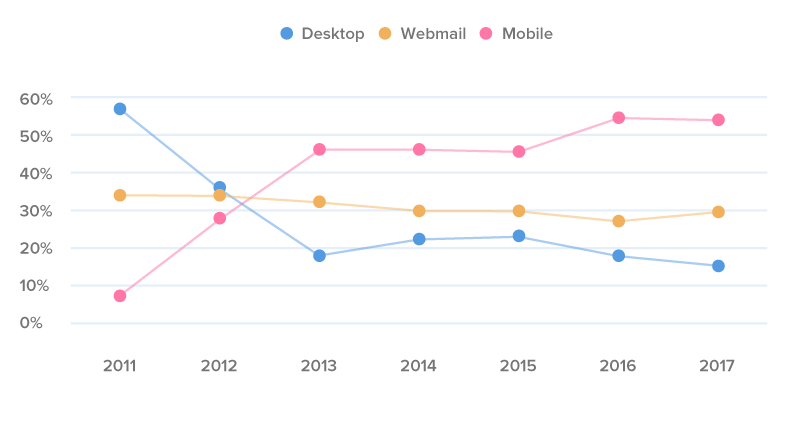
\includegraphics[width=\textwidth]{img/popularity.png}
\caption{Comparison of popularity progress of different categories of e-mail clients}
\label{fig:popularity}
\end{figure}
The popularity of the web-based and mobile clients is caused mainly by the simplicity of their deployment (no complicated configuration is usually required for their use) and the integration of many vendor-specific improvements, like search services, inter-device sharing or high availability of the service.

Despite the advantages of such interfaces, many users are forced to use less advanced solutions due to various limitations: For example, a company may choose not to submit confidential communication to its e-mail provider. Similarly, a single user may wish to process his e-mail communication locally, to avoid the issues with connectivity or provider reliability.

Such users usually deploy open-source solutions which effectively solve both the problem of vendor trust (because the software can be audited easily) and local maintainability. On the other hand, the numerous useful features (such as high-performance full-text search) and the mentioned vendor-specific improvements are typically missing in the open-source solutions.

This thesis is motivated by the concept of e-mail handling that was introduced by Google for Gmail and subsequently improved by Google Inbox. The approach completely replaces the handling of mail folders for mail organization by a more flexible use of customizable tags, and makes heavy use of Google's full-text search facilities.
Open-source solutions that would implement a decent alternative to Google Inbox are, to the best of author's knowledge, currently missing.
On the other hand, recent open-source developments have created several search engines and databases that can be used to support the underlying storage and search capabilities. Therefore, development of the alternative is possible by connecting this functionality to e-mail processing infrastructure and providing a matching modern interface for the end-user.

The goal of this thesis is to create this alternative. The specific aims include the following:
\begin{itemize}
\item high speed search for Google-like queries in large amounts of e-mails, including the tag functionality
\item integration with the e-mail processing infrastructure --- receiving, parsing, formatting and sending of e-mails
\item storing the e-mails in a reliable database
\item support for multiple users and account management
\item web-based user interface comparable to modern commercial solutions, using modern UI toolkits and frameworks to promote extensibility
\end{itemize}
The resulting open-source software package is called KamehaMail. It is possible to run KamehaMail on any modern UNIX operating system with a modern working mail server (including exim or postfix). The search functionality is provided by open-source search-engine database ElasticSearch.

This thesis is structured as follows: \Cref{mailprocess} describes the processing of e-mail messages and related Internet infrastructure. \Cref{textsearch} details the functionality of full-text search databases and their deployment in the real environments. \Cref{implementation} describes the implementation of KamehaMail, including the implementation of the backend (server part) and browser-based frontend. Performance of the resulting software is briefly benchmarked in \cref{results}. After conclusion, a short installation and user guide is provided in \cref{userguide}.

\paragraph{Related Work and Software.}
There exist a great amount of open-source web-based e-mail interfaces, such as squirrelmail, roundcube, rainloop, mailspring or notmuch-web. Most of them support full-text search using IMAP search or other own means. Yet, the handling of the e-mails as its done by Google Inbox is on whole different level on both end-user's side and the functional side. KamehaMail is trying to be as close as possible to the commercial interfaces while implementing open-source tools.

\chapter{Electronic mail processing}
\label{mailprocess}
E-mail or Electronic mail is a mean for sending and receiving messages between two users on the internet. To process an e-mail, it is necessary to understand the format of e-mail message as defined by multiple RFCs (Request for Comments). Generally, an e-mail is a text document separated into a header and a body. The header contains meta-information about the e-mail, the body contains the actual message. Encoding of the messages is further explained in the 
\autoref{mime}.

This chapter describes the important parts of the format for the processing of an e-mail message as defined by RFC 5322~\cite{rfc5322}, the protocols that define the e-mail communication (SMTP, IMAP and POP), and the transfer agents that make use of these protocols and ensure the communication.

\section{History}
First use of electronic messages as a form of communication can be traced back to early 1960s\footnote{\texttt{http://www.nethistory.info/History\%20of\%20the\%20Internet/email.html}}. Using the Compatible Time-Sharing System, hundreds of users at the MIT Computation Center could log into the remote dial-up terminals to store their files.
This way of sharing data encouraged new ways of communication to be invented. The \texttt{mail} command for the CTSS was written in the 1965 to work with e-mail within a single computer.

Ray Tomlinson is considered to be the creator of the e-mail: He was the first one to use the symbol @ for denoting a message to be sent between the computers on ARPANET in 1972. Since then, ARPANET encouraged the usage of e-mails which quickly became widespread. Soon after, the protocols and tools for the foldering and e-mail organization were invented.

Historically, one of the most important e-mail standards is \emph{Simple Message Transfer Protocol} (\emph{SMTP}), defined in the 1982. Starting as a complement to the already existing \emph{Unix to Unix Copy Program} (\emph{UUCP}), SMTP soon started to be widely used. Nowadays, majority of the e-mail communication is done via SMTP.  Nevertheless, the protocol is designed only for the message-pushing transfers. Additional protocols are required to support other use-cases.

\emph{Post Office Protocol} (shortly \emph{POP}) appeared in the 1984. It was an important standard as it stated the rules of an e-mail message retrieval to personal computers, which consequently helped to standardize the communication between the user and the mail server. Nowadays, the most used internet protocols for e-mail communication are POP3, IMAP and SMTP, further discussed in \autoref{smtp} and \autoref{popimap}.

\section{Message Format}
Multiple standards defining the e-mail message format were created throughout the years. Probably the most important one was defined by RFC 822, as it was the first protocol standardizing the e-mail message format. 20 years after being published, it was replaced by RFC 2822 in the 2005 which was later obsoleted in the 2008 by RFC 5322.
The following sections summarize the current e-mail format standard, defined by RFC 5322~\cite{rfc5322}.

E-mail message, as defined by RFC 5322, is split into two major parts, the \emph{header} and the \emph{body}.

\subsection{Header}
The \emph{header} is composed of \emph{fields} that contain meta-information about the e-mail (e.g. subject of the message, sender of the message\dots).
Field is a pair of two text values separated by a colon:
\begin{center}
\texttt{field name: field value}
\end{center}
If a line in the header begins with 7-bit ASCII character, it is a field. If a line starts with white space, the value of the field from the previous line continues on the current line, which makes multi-line fields possible. The values of the fields have to be 7-bit ASCII as well. To encode a non-ASCII value of a field, \emph{MIME} encoding is used. 

\label{mime}
\emph{MIME} is a standard that describes the encoding of non-ASCII values to 7-bit ASCII (e.g. to support multiple different charsets or structured values). To encode a string in a different charset, the following syntax is used:
\begin{center}
\texttt{=?charset?encoding?encoded text?=}
\end{center}
For example:
\begin{center}
\texttt{=?iso-8859-1?Q?=A1Hola,\_se=F1or!?=}
\end{center}
After decoding the encoded text using the provided charset and the encoding, we obtain the value \texttt{¡Hola, señor!}. A typical use of the MIME encoding is the support for different languages.

Only two header fields are mandatory for each message: \texttt{Date} and \texttt{From}. All other fields are optional, however, there are several fields that are recommended and several fields that are commonly used. Most of these fields are described in \autoref{table:fields}. 
\begin{table}[t]
\centering
\renewcommand{\arraystretch}{1.4}
\begin{tabular}{l p{20em}}
 \toprule
 Field name & Description\\
\midrule
 \texttt{Date} & Date of origination (mandatory)\\
 \texttt{From} & Address of the sender (mandatory)\\
 \texttt{Message-ID} & Recommended for the message identification\\
 \texttt{In-Reply-To} & Recommended, if the message is a reply\\
 \texttt{References} & Recommended, if the message references to other messages\\
 \texttt{Sender} & Displayed sender (optional)\\
 \texttt{Reply-To} & The address to reply (optional)\\
 \texttt{To} & Displayed recipient (optional)\\
 \texttt{Cc} & Carbon Copy, used for sending copies of e-mail to multiple users (optional)\\
 \texttt{Bcc} & Blind Carbon Copy, same as Cc except the recipients are not visible (optional)\\
 \texttt{Subject} & Subject of the message (optional)\\
 \texttt{Return-Path} & Return address (optional)\\
\bottomrule
\end{tabular}
\caption{Header fields as defined by RFC 5322.}
\label{table:fields}
\end{table}
A detail worth mentioning is that the \texttt{To} and \texttt{From} fields do not have to necessarily be the same addresses as the actual sender and recipient addresses. These fields are just informative, the real addresses are given to the SMTP for the mail delivery. SMTP is described further in \autoref{smtp}. 

An example of headers of a real e-mail message is displayed in \autoref{fig:message}.
\begin{figure}
\centering
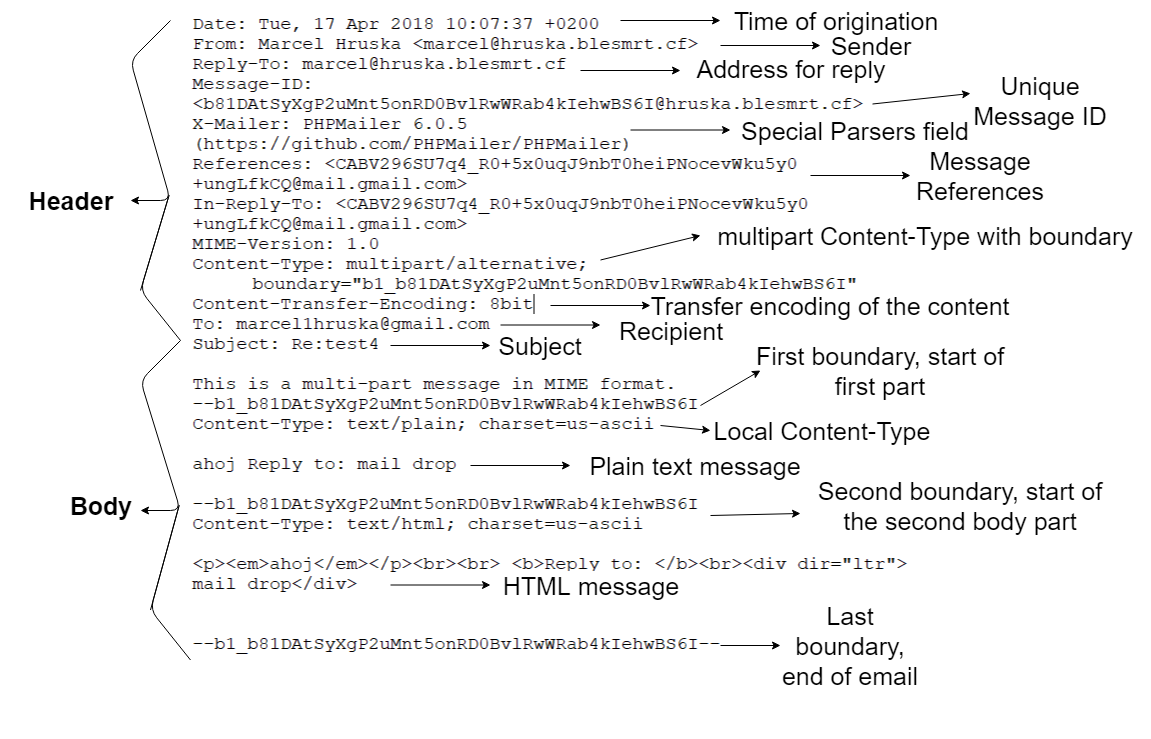
\includegraphics[width=\textwidth]{img/message_example.png}
\caption{A message sent from KamehaMail to a user of Gmail.}
\label{fig:message}
\end{figure}

\subsection{Body}
This section describes the format of the content of the message, called body.
RFC 5322 does not describe an exact format of message body, but references other documents for this purpose. For example, RFC 2045~\cite{rfc2045} from 1996 describes how the body of the message is supposed to look (its format, syntax\dots). We cover only the parts of RFC 2045 necessary for the purposes of this thesis.
The body is separated from the header by one blank line.

Originally, the messages were meant to be plain-text 7-bit ASCII only. However, it is possible to use the MIME encoding for the message bodies as well. 

If the user decides to use the MIME encoding for the message body, three header fields must be filled in: \texttt{MIME-Version}, \texttt{Content-Type} and \texttt{Content-Transfer-Encoding}.

\texttt{MIME-Version} is the version of the MIME being used for the encoding of the message, currently \texttt{1.0}.

\texttt{Content-Transfer-Encoding} specifies the encoding of the body. For example, SMTP expects messages to be 7-bit US-ASCII, which can be changed to 8-bit encoding using this header, making successive encoding more convenient.

\texttt{Content-Type} describes the type of data so that the receiving part understands how to decode the contents of the e-mail properly. This value is called \emph{media type}. Each media type has its subtype identifier, which further refines the media type. After the type identifiers comes a semicolon and parameters, if necessary. For example,
\begin{center}
\texttt{Content-type: text/plain; charset="us-ascii"}
\end{center}
defines media type \texttt{text}, its subtype \texttt{plain} and the parameter defining the charset \texttt{charset="us-ascii"}. This is also the default value, if the header is not present.

\subsubsection{Multipart messages}
There is a commonly used media type that we want to mention specifically, described by RFC 1341~\cite{rfc1341}, called \emph{multipart}.
The multipart content-type allows to combine multiple bodies/body parts in a single message, each possibly encoded in a different way. Vast majority of the modern e-mail clients uses it to send two bodies: an HTML body for the user interfaces that are capable of displaying HTML messages, and a plain-text body for the compatibility with simple plain-text interfaces.
Another widespread use of the multipart media type is to encode the attachments into the body of the e-mail.

All subtypes of the multipart content-type follow the same syntax. The header must specify a parameter called \emph{boundary}, which is used to separate the body parts by two hyphens and the boundary string. Each of the separated body parts has its own content-type header defining its inner message type. The syntax of multipart content-type is displayed in the example in \autoref{fig:message}.

\section{Message exchange}
Because it is too complicated to send a message directly to end recipient's computer with knowing only his e-mail address, a more complicated infrastructure is used for e-mail delivery. 
The computers in this infrastructure are classified by the role they have as \emph{Mail Transfer agents} (MTA), \emph{Mail User Agents} (MUA), \emph{Mail Delivery Agents} (MDA) and \emph{Mail Submission Agents} (MSA).

This section gives a closer description of the roles of e-mail agents and the communication protocols that the e-mail agents use.

\subsection{E-mail Agents}
The end-to-end delivery of a message has several stages: the submission of the message, the transfer of the message and the retrieval. Many complications can occur during the transport, such as non-existing final destination or disconnected user. \emph{E-mail agents} were invented to take care of these situations which are futher detailed in the following sections as defined by RFC 5598~\cite{rfc5598}.

\subsubsection{Mail Transfer Agent}
\emph{Mail Transfer Agent} (also known as \emph{Mail Server}) is designed to transfer e-mail messages, implementing both sending and receiving parts of the SMTP protocol.
It is often called a mail relay as well because its job is to route and forward e-mails to their final destinations.

MTAs are running in the background. They are listening to a port, waiting for the message to come, either from another MTA or from the user. If the message comes from another MTA, it is either routed to the next MTA on its path or in case that the current MTA is its final destination, stored locally for the user. 
UNIX mail servers exim, postfix or sendmail are all examples of MTAs.

MTA does not implement the access to the messages for the user, which needs to be handled by different agents.

\subsubsection{MUA, MSA, MDA}
For the communication between the user and the MTA, \emph{Mail User Agent} (also known as \emph{e-mail client}) is used. MUA 's main role is to retrieve e-mails from the MTA for the user and display them. It often implements the interface for the composition of an e-mail. E-mails created by an e-mail client are then sent to the corresponding MTA for distribution.
Usually, the communication between MUA and MTA is not direct. Two more systems are commonly used as a layer between MUA and MTA: \emph{Mail Submission Agent} and \emph{Mail Delivery Agent}.

MSA takes care of the submission of a message from MUA to MTA. It uses SMTP as well but listens to a different port. Some of the advantages of having an MSA are the following: It enforces the policies of the standard protocols while representing the interests of the author of the message. It rejects messages that do not satisfy the conditions stated by the internet standards. It includes header fields such as \texttt{Date} or \texttt{Message-ID}. In some cases, it can help to solve minor errors.

MDA takes responsibility of storing an e-mail for the user from MTA and delivers the message to the recipient's MUA. Common role of the MDA is to redirect the message to user-defined address. 

A simple diagram of the e-mail flow is shown in the \autoref{fig:mail-flow}.
 \begin{figure}
\centering
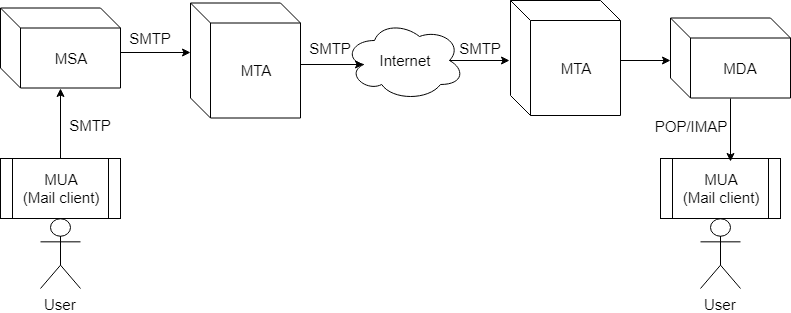
\includegraphics[width=\textwidth]{img/mail_flow.png}
\caption{A simple diagram of the e-mail transfer flow between two users.}
\label{fig:mail-flow}
\end{figure}
The transfer of the messages between two MTAs is defined by SMTP. The retrieval of the message to the MUA is done using IMAP or POP.

\subsection{E-mail protocols}
\subsubsection{SMTP}
\label{smtp}
In the previous sections, we mentioned the internet protocol SMTP which is a standard for an e-mail transfer. It was first defined in the 1982 by RFC 821~\cite{rfc821} and last updated in the 2008 by RFC 5321.
SMTP defines a model of communication as follows: The user sends a request to the sender-SMTP\footnote{sender-SMTP and receiver-SMTP are servers capable of communicating via SMTP, usually MTA} to start an e-mail communication. The sender-SMTP opens a two-way communication with the corresponding receiver-SMTP which is either an intermediate or the final destination. After that, the user can submit mail commands via the established communication path and receive the responses.
The \autoref{fig:smtp-model} shows the SMTP model as described by RFC 821.
\begin{figure}
\centering
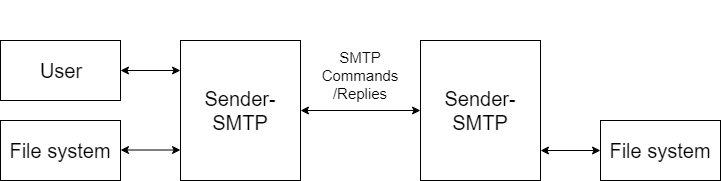
\includegraphics[width=\textwidth]{img/smtp_model.png}
\caption{Model for SMTP use.}
\label{fig:smtp-model}
\end{figure}

To begin an e-mail transaction, user introduces himself using \texttt{HELO} command. Then there are three stages of the SMTP mail transaction.
\begin{enumerate}
\item The first part is the \texttt{MAIL} command. This command indicates the beginning of a new e-mail transaction for the receiver-SMTP. The receiver-SMTP resets all the state data it has and prepares for the following commands corresponding to the new transaction.
\begin{center}
\texttt{MAIL <SP> FROM:<reverse-path> <CRLF>}
\end{center}
Tags \texttt{SP} and \texttt{CRLF} mean space and an end-of-line respectively. The \texttt{reverse-path} in the field \texttt{FROM} contains address where the responses will be sent, for example errors. If the command was processed successfully, the response \texttt{250 OK} is sent to the return address.
\item The second part is the \texttt{RCPT} command which defines the receiving address of the current mail transaction. 
\begin{center}
\texttt{RCPT <SP> FROM:<forward-path> <CRLF>}
\end{center}
The \texttt{forward-path} contains the address of the recipient. If the receiver-SMTP does not recognize the address, it responds with \texttt{550 Failure}. This command can be repeated for multiple recipients. If accepted, the \texttt{250 OK} reply is sent.
\item The third and the last part is the \texttt{DATA} command. This command transfers the actual data of the message.
\begin{center}
\texttt{DATA <CRLF>}
\end{center}
If the command is accepted by the receiver-SMTP, the reply \\ \texttt{354 Intermediate} \\ is sent. All following lines until the end of the text are the data of the message. The headers of the message are sent via \texttt{DATA} command as well.
\end{enumerate}
To end the transaction, the \texttt{QUIT} command is used.
The whole process is summarized in the following example~\cite{rfc821}:
\\
\texttt{S: HELO client.example.com}\\
\texttt{R: 250 Hello client.example.com}\\
\texttt{S: MAIL FROM:<Smith@Alpha.ARPA>}\\
\texttt{R: 250 OK}\\
\\
\texttt{S: RCPT TO:<Jones@Beta.ARPA>}\\
\texttt{R: 250 OK}\\
\\
\texttt{S: RCPT TO:<Green@Beta.ARPA>}\\
\texttt{R: 550 No such user here}\\
\\
\texttt{S: RCPT TO:<Brown@Beta.ARPA>}\\
\texttt{R: 250 OK}\\
\\
\texttt{S: DATA}\\
\texttt{R: 354 Start mail input; end with <CRLF>.<CRLF>}\\
\texttt{S: Blah blah blah...}\\
\texttt{S: ...etc. etc. etc.}\\
\texttt{S: <CRLF>.<CRLF>}\\
\texttt{R: 250 OK}\\
\texttt{S: QUIT}\\
\texttt{R: 221 Bye}\\
\label{mail-command}
There exists many other commands that SMTP protocol uses for the communication. However, this is all handled by MTA.

\subsubsection{POP and IMAP}
\label{popimap}
IMAP was defined by RFC 3501 in the 2003 and its current version is IMAP4~\cite{rfc3501}. POP was first specified by RFC 918 in the 1984 and its current version POP3 was defined by RFC 1939 in the 1996~\cite{rfc1939}. While they are both protocols designed for message retrieval for the e-mail client from mail server, POP is much older than IMAP.

The main difference between them is that IMAP is designed for multi-device use (tablet, phone, desktop\dots), displaying the same content on any device since the content is synchronized on the central server. POP is designed for downloading the e-mail from the mail server to the local machine without any synchronization. What's more, POP can be set to remove the messages from the server after download. In reality, both of the protocols can be setup to work in a very similar way. However, POP is unable to tell if the message was read or not or to provide meta-information about the existence of a folder.

Both provide advantages and disadvantages for the user. IMAP is more simple to set up for multi-device use as it does not create local storages of messages on every used device. However, usage of POP offers certain degree of privacy as the e-mails can be removed from the server after their download.

\section{End-user interfaces}
This section briefly describes end-user's phase of the e-mail transfer flow. An interface has to be provided for the user to interact with the mail server and retrieve or send e-mails. E-mail interfaces can be classified by the type of the interaction and the localization of the data.

\subsection{Desktop clients}
To proceed chronologically, the first e-mail clients described in this section are so-called \emph{desktop clients}. It is a common name for all clients that are installed on the user's machine and work with the messages locally, using the message retrieval protocols. They can be further subdivided into \emph{command-line} clients and clients with \emph{graphical user interface}.

\subsubsection{Command-line clients}
Historically, the first e-mails ever were sent using console commands. \emph{Com\-mand-line} clients provide only basic graphical interface for the user. We have already presented an example of SMTP \texttt{mail} command in the \autoref{mail-command}.
Although the command-line clients are an old technology, they are not extinct. On the contrary, they are still popular because of the safety reasons (no HTML and JavaScript), speed reasons (graphical interfaces take longer to load and respond) and the flexibility. For example, UNIX's \texttt{mail} command is still being frequently used.

\subsubsection{GUI clients}
As the displaying units grew bigger, e-mail clients with more advanced graphical user interfaces became popular. These are well-known by the average e-mail users as they are more user-friendly to use than the command-line clients. Some of the most popular e-mail clients are Mozilla Thunderbird or Microsoft Outlook. 

\subsection{Web based clients}
Another category of the e-mail clients are \emph{web based} clients or simply \emph{webmails}. The major difference between the desktop clients and the web based clients is that no e-mails are being downloaded locally to the user's computer. Instead, they are stored to the webserver and can be accessed by the user via web browser.
The first webmail was developed at CERN in 1993 by Hallam-Baker Phillip called The Mail Server Daemon~\cite{cern-mail}. Bigger development of the webmails began with the easier access to the Web in the 1990s an 2000s. 
However, using a web browser as an interface represents a certain level of threat because the communication over unsecured HTTP can be readable by third parties. Usage of encrypted HTTPS communication is highly recommended.
Some of the most popular webmail services are Gmail, Outlook.com and Yahoo! Mail and some of the most popular open-source webmails are squirrelmail, roundcube, rainloop, mailspring, notmuch-web\dots

\subsection{Mobile clients}
Currently, there is a new category, \emph{mobile} e-mail clients. Smart phones are incredibly popular and the mobile clients dominate e-mail client market share. Around 55\% of the e-mails were opened on mobile phones in the 2016\footnote{\texttt{https://litmus.com/blog/the-top-10-most-popular-email-clients-of-2016}}. They are very similar to the desktop clients, except that mobile clients are optimized for smaller touch screens.

\chapter{Text search}
\label{textsearch}
In order to create a modern, searchable e-mail interface, it is necessary to implement an algorithm that retrieves the wanted information quickly from a great amount of e-mails. The e-mail databases of some of the e-mail providers, such as Google or Outlook.com, have grown incredibly big throughout the years, containing billions of e-mails. Such databases are often far too big for naive approaches --- to find an email that contains specific keywords quickly (in milliseconds) we need a proper research of more advanced solutions for this problem.

This chapter describes the \emph{Text search}, its use in the search engines, its advantages and disadvantages comparing to the standard database search, its principles of use and implementation. 

Generally, the text search is used to find a document that contains a specific word structure in a database of text documents. In this chapter, we describe the overall process of \emph{indexing} the documents in such a database, and searching through them.

A \emph{document} is a single file of words, usually plain-text, processed and stored in the database: They are preprocessed before getting stored in order to simplify the search processing, for example by removing some unwanted (irrelevant for search) parts of the original text, such as various auxiliary words\footnote{Including e.g. articles, prepositions and conjunctions, these are usually called stop-words.} or markup, and split into so-called \emph{terms}. The terms are `clean' representations of the document content which are then stored in the database, together with the identification of the document they originated from. The list of split and processed terms associated to their documents is usually called a \emph{text-search index}. We describe this preprocessing, also usually called \emph{text analysis}, closer in \autoref{analysis}; indexing is described later in \autoref{index}.

The preprocessing of the document, as well as the searching itself, is usually done by a \emph{search engine}. A search engine is a system that integrates many text-search-related techniques to provide a coherent implementation of the indexing and querying functionality. In \autoref{engines}, we explain closer how the modern search engines work: The user requests sent to the search engine are called \emph{queries}. Each query lists some requested text words together with additional search criteria. The text in the query is processed by the same analysis that the documents are, to produce a simplified query of terms suitable for looking up in the database. The \emph{match} is the result of the search that is returned by the search engine as an answer to the given query. In other words, the match is a list of documents (in the most basic case it only contains document IDs) that
satisfy the criteria given by the query (e.g. contain the requested words).

Some search engines allow to structure the inner contents of the documents into \emph{fields}: Instead of treating all terms equivalently, users may separate them into the sets represented by the fields. A field is usually identified by string name, and contains a separately-searchable text value. For example, library databases may use fields such as \texttt{title}, \texttt{authors} or \texttt{topic}. This not only simplifies the user interface of the search, but also lowers the amount of data that need to be examined by the engine upon processing the query, because only the specific fields may be examined.

A simple diagram of the whole search cycle is provided in \autoref{fig:basic-chart}.
\begin{figure}
\centering
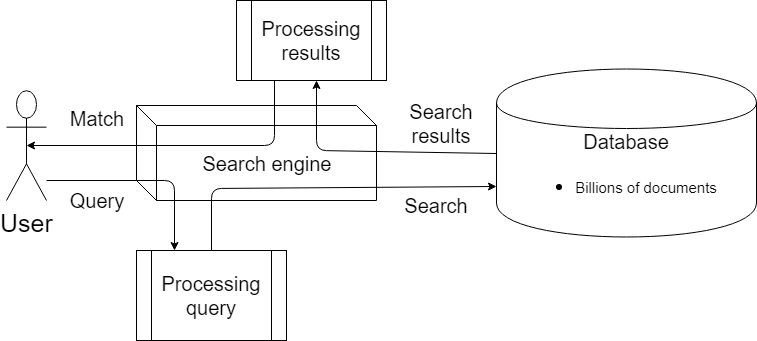
\includegraphics[width=\textwidth]{img/basic_chart.png}
\caption{A simplified view of the search cycle.}
\label{fig:basic-chart}
\end{figure}

In the following sections, we explain how the text search actually works, what processes are necessary for it to work efficiently and how to implement it.


\section{Text analysis}
\label{analysis}
There are many problems with word matching. Should  "ring" and  "Ring" match? Or  "swear" and  "swears"? In the natural human perception, we know that simply having the word at the beginning of the sentence (i.e. capitalized) does not change the meaning of the word. It is the same word as its non-capital version. We learned that "swear" and  "swears" are the same word, just in a different form. The search engine does not know that and we have to provide him with exact rules that he processes the words of the text as similarly to our perception as possible. This process is called \emph{text analysis}

Before we store the terms into the index, we need to preprocess them.
The text search analyzers are systems that process the words of the text and store them into the index. In reality, it is quite common that they treat the data in a natural way. Standard analyzers could remember the relative position, skip the insignificant words (such as "the"), treat certain fields as an exact type (e.g. date). Depending on the language, the analyzers can also decide to store the same word for its different word forms. For example, both words "forgot" and "forgotten" can be placed under the word "forget".

Generally, there are two phases of the text analysis, the \emph{tokenization} and the \emph{mapping}. \emph{Tokenization} is mandatory for creating the index but \emph{mapping} is optional and used only when needed.

The tokenization of the string is further subdivided into the following stages~\cite{elastic}.
\begin{enumerate}
\item First stage is the \emph{characters filter}. It is a preprocessing of the text before tokenization. It converts the text to the form that will be more simple to tokenize. For example, it is used to strip out HTML tags or convert \& to "add".
\item Then comes the tokenization itself. The string is split into the individual terms, accordingly to the defined analyzing parameters. The most simple tokenizers split the text whenever they encounter punctuation or whitespace, while removing the delimiter from the term.
\item The last stage is similar to the characters filter, the terms are post-processed by the \emph{tokens filter}. These filters change terms into their simplified forms, such as base forms, for easier future searching. The most common filters are lowercasing, removing the words with no possible significance to the search (stop words, e.g. "and", "the" etc.) or even adding words, such as synonyms.
\end{enumerate}

\subsection{Mapping}
As we mentioned before, there is more to the text analysis than the tokenization. We can tell the search engine how to treat specific fields and their values. For example, it is possible to have a field that contains only numbers. The search engine should understand that the value is not a simple plain string but a number. Later, it can make use of this type. For instance, the search engine can sort the results by this field. This technique is called mapping. 

Mapping is the process of defining how a document, and the fields it contains, are stored and indexed~\cite{elastic}. Which fields should be full-text fields, which should be numbers, booleans, date values, or not analyzed at all. Some search engines, for example ElasticSearch, offers the possibility to map a field using a specific language analyzer. If a field is supposed to contain only french words, the analyzer can understand the syntax of the French language and match it accordingly. For example, the word "anneau" ("ring" in English) and the word "Anneaux" have the same base form for the French language analyzer. The English language analyzer has a very little chance to understand that. Search engine remembers the specific settings for each field and processes the queries against them accordingly as well.

Different search engines use different approaches to the text analysis. How deeply is the text to be processed is mainly up to the developer that sets up the search engine.
For the purposes of this thesis, the most convenient way was to analyze almost every field. We wanted that the date of received/sent e-mail is treated as a date (milliseconds since certain date in the past) and that the results can be sorted by this value. On the other hand, there was no need to analyze fields such as \texttt{messageid} since in order to find a match, we are supposed to know the exact value. 
We did not specify any language analyzer as the users of KamehaMail can be of different nationalities, consequently writing their e-mails in different languages.

We used tokenization and mapping to process the text into terms and now we want to store them.
\section{Indexing and inverted indexes}
\label{index}
Much research has been performed to design efficient
index structures for database and information retrieval
systems~\cite{structs}. There was a need to find an ideal data structure to store and retrieve data from a database full of plain-text documents as quickly as possible. In order to do reach the solution, some sort of indexing of the split terms was needed.
A standard forward index appeared to be inefficient for the full-text search. The goal is not to look for the documents but for the words in them. Thus, the most efficient index structure is an \emph{inverted index}~\cite{invertedfiles}.

An \emph{inverted index} is structured the opposite way to the forward index. Instead of having a list of documents along with lists of terms accordingly, inverted index contains a list of terms and for each the documents that contain them. The difference between them is shown in the \autoref{table:forward-inverted}.

\begin{table}[t]
\centering
\renewcommand{\arraystretch}{1.4}
\begin{tabular}{c l}
\toprule
Inverted Index\\
\midrule
Term 1 & List of documents \\
Term 2 & List of documents \\
Term 3 & List of documents \\
Term 4 & List of documents \\
\dots & \dots \\
\bottomrule
\end{tabular}
\qquad
\begin{tabular}{c l}
\toprule
Forward Index\\
\midrule
Document 1 & List of terms \\
Document 2 & List of terms \\
Document 3 & List of terms \\
Document 4 & List of terms \\
\dots & \dots \\
\bottomrule
\end{tabular}
\caption{An inverted index (left) and a forward index (right).} 
\label{table:forward-inverted}
\end{table}

There exist two major types of inverted indexes. An \emph{inverted file} (or \emph{document-level index}) and a \emph{full inverted index} (or \emph{term-level index}). The difference is that inverted file is used only for accessing the documents of the corresponding term. It is sufficient when no other information than document's ID is needed. A full inverted index has complete information about the term in the file (e.g. position) which makes it far bigger and harder to maintain, however indispensable in certain use cases, for example, when the word position is needed.

An inverted index consists of two main parts.
\begin{enumerate}
\item The first part is the \emph{vocabulary}. It is a list of all distinct terms of all documents. Each of them can contain information about document count and about their \emph{inverted lists}. The inverted lists are associated to their respective terms directly, as a list or by a pointer to the corresponding part. The position of a word is stored as well, if it is not the document-level index. This list is ordered.
\item The second part is an \emph{inverted list} which is a list of all documents where the word appeared. These lists can be represented as pairs \((d, f_{d,t})\) where \(d\) represents the identifier of the document and  \(f_{d,t}\) is the associated set of frequencies of the term \(t\) in the document \(d\)~\cite{invertedfiles}.
This list is ordered as well.
\end{enumerate}

A simple database of documents is provided in the \autoref{table:data-ex} for the presentation purposes. Each document in the table is uniquely identified by its \texttt{ID} field. The actual text of the quote is stored in the \texttt{Text} field. The \texttt{Author} field contains the author of the quote. As we mentioned before, the terms are processed and stored to the index structure which is shown in \autoref{table:invlist-ex}. Notice that the inverted index provided in the example is made only of the field \texttt{Text}.

\begin{table}[t]
\centering
\renewcommand{\arraystretch}{1.4}
\begin{tabular}{c p{20em} l}
\toprule
ID & Text & Author\\
\midrule
1 & Your time will come. You will face the same Evil, and you will defeat it. & Arwen \\
2 & The Ring has awoken, it has heard its masters call. & Gandalf \\
3 & We swears, to serve the master of the Precious. We will swear on\dots on the Precious! & Gollum \\
4 & You shall not pass! & Gandalf \\
\bottomrule
\end{tabular}
\caption{A simple database of quotes from Lord of the Rings.} 
\label{table:data-ex}
\end{table}

\begin{table}[t]
\renewcommand{\arraystretch}{1.4}
\resizebox{\textwidth}{!}{
 \begin{tabular}{c c} 
 \toprule
 term \(t\) & \((d, f_{d,t})\) \\ 
 \midrule
 and & (1, 1) \\
 awoken & (2, 1) \\
 call & (2, 1) \\
 come & (1, 1) \\
 defeat & (1, 1) \\
 evil & (1, 1) \\
 face & (2, 1) \\
 has & (2, 2) \\
 heard & (2, 1) \\
 it & (1, 1),  (2, 1) \\
 its & (2, 1) \\
\bottomrule
\end{tabular}
\quad
 \begin{tabular}{c c} 
 \toprule
 term \(t\) & \((d, f_{d,t})\) \\ 
 \midrule
 master & (3, 1) \\
 masters & (2, 1) \\
 not & (4, 1) \\
 of & (3, 1) \\
 on & (3, 2) \\ 
 pass & (4, 1) \\
 precious & (3, 2) \\
 ring & (2, 1) \\
 same & (1, 1) \\
 serve & (3, 1) \\
 shall & (4, 1) \\
\bottomrule
\end{tabular}
\quad
 \begin{tabular}{c c} 
 \toprule
 term \(t\) & \((d, f_{d,t})\) \\ 
 \midrule
 swear & (3, 1) \\
 swears & (3, 1) \\
 the & (1, 1),  (2, 1),  (3, 3) \\
 time & (1, 1) \\
 to & (3, 1) \\
 we & (3, 2) \\
 will & (1, 3),  (3, 1) \\
 you & (1, 2), (4, 1) \\
 your & (1, 1) \\
 & \\
 & \\
\bottomrule
\end{tabular}
}
\caption{A document-level inverted index for the database shown in the \autoref{table:data-ex} with only word occurrences.}
\label{table:invlist-ex}
\end{table}

Nowadays, there are plenty of variations for the inverted index structure. Several possibilities were mentioned in the article written by Mahapatra and Biswas~\cite{invindex}. For instance, some of them store meta data. Apart from the additional information stored for each word (such as the frequency of the occurrence or the word position), these implementations contain meta-information about each hit. \emph{Hit} is an exact word position in the document. These meta data may contain information such as font type, font size, text type etc\dots Other solutions mentioned in the article implement both types of the inverted indexes, the full inverted index and the inverted file, each for different situations.

Creating an inverted index is a simple task. However, it can be challenging to create it without wasting memory and CPU. Advancements in the hardware do not provide any significant help because the collections are growing in size even faster. An efficient way is needed for creating, storing and maintaining the index.

\subsection{Construction of inverted index}
The fastest and the most simple way to construct an inverted index is to build the whole collection in memory. However, this approach is not possible for bigger collection (i.e. billions of documents, terabytes of data). Such collections do not fit in the memory and disk has to be used which is always costly. An optimized method that
creates small, memory fittable inverted lists, stores them to disk and merges them when all is done is needed. Moffat and Bell or Heinz and Zobel described several methods solving this problem~\cite{invindex}.

\subsection{Structure of the inverted index}
The article written in 1996~\cite{structs} defines two following approaches for the inverted index structures.

The first approach is to maintain an inverted index only for the document access. Specifically, only document IDs are returned upon a matching query. A postprocessing is needed to retrieve additional information about the document, if wanted. That is done by using a term-level index. This approach has a significant disadvantage, as the number of the matching documents can be large, the postprocessing can be time consuming. Although, it can be improved by using an internal tree representation.

The second approach is about having an index for each element type. It may create a huge space overhead as each term must appear in every index. There were attempts for removing the duplicates, for example by using a combined vocabulary. Nevertheless, the space overhead was still far too great.
Many different possible structures exist which take care of the duplicates and improve the consequential space overhead.

To further reduce space consumption, compressions can be applied on the inverted lists~\cite{invindex}. For example, instead of storing all the numbers as 32-bit integers, variable-length numbers can be used.

\subsection{Segmentation}
The maintenance of already existing inverted index also causes an issue. Inserting a new element into a sorted list and updating the whole index with possibly billions of documents directly is too expensive.

ElasticSearch uses the principles of \emph{segmentation} as defined by Lucene and the following facts will be interpreted as explained in the guide for ElasticSearch~\cite{elastic}. 

Instead of rewriting the whole inverted index again upon each new entry, completely new indexes are created with the recent results. Such supplementary index is called a \emph{segment}. Lucene describes the index as a collection of segments and a commit point. Commit point serves as a common entry point for its segments, the query is performed against it, the commit point then distributes the query to all its segments and returns the results combined.
The \autoref{fig:commit} shows an example of the segmentation.
\begin{figure}
\centering
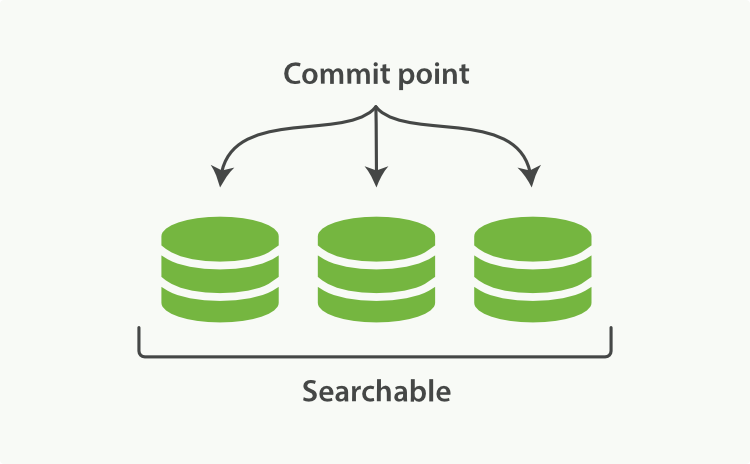
\includegraphics[width=.8\textwidth]{img/commit.png}
\caption{A commit point for three segments of the index.}
\label{fig:commit}
\end{figure}
This may cause an issue because the approach may create an enormous amount of small segments which consume additional CPU and memory, rendering inverted indexes inefficient.
It can be at least partially improved by merging the segments, transparently for the incoming search query and the user. It is most convenient to run this process when a new, not yet committed (not yet written to the specific commit point) segment has been set. Currently committed segments are taken along with the new uncommitted one and merged. The new merged segment is then committed into the commit point and the old ones are to be removed. To remove them safely, the search engine must be sure that there are no searches being performed on them which usually delays their removal.

The problems mentioned above are not the only problems concerning inverted indexes. However, they are efficiently solved by the search engine we integrated to the application, ElasticSearch. The specifications of ElasticSearch are mentioned in \autoref{es}. 

\section{Query structure}
\label{query}
Once the database is constructed and prepared for the text search queries, it is possible to search in it. Search engines usually provide an API to make the communication with them (i.e. send the queries and receive the match data) possible. The following examples are written in a JSON-based syntax, similar to the ElasticSearch~\cite{elastic} but simplified for presentation purposes. The queries are effectively performed against the inverted index to the database shown in \autoref{table:data-ex}. The \texttt{Text} field part of the database is displayed in \autoref{table:invlist-ex}.

A simple query looking for the term "ring" is shown in the following example:
\begin{code}
{ "query": { 
    "term" : "ring"
} }
\end{code}
The second document contains term "ring" and it is the only match. The most basic result to the above query returns only the matched documents' IDs:
\begin{code}
{ "hits": [
    { "ID" : 2 } ] 
}
\end{code}
\texttt{Hits} is an array of results. For each matching document, it contains at least the document's ID. Nonetheless, there are cases where we want to have more information about the document than its ID. For example, other contents of the matching documents or the relevancy of the document to the given query.

Queries can be more complex, defining different logical search criteria. We can use logical NOT (for the unwanted terms), AND (for multiple terms) and OR (for optional matches). In the following example, user is looking for those documents that contain terms "master" and "precious", cannot contain term "ring" and optionally may contain term "evil":
\newpage
\begin{code}
{ "query" : { 
     "bool" : {
       "must" : {
        "term" : "precious",
        "term" : "master"
      },  "must_not" : {
        "term" : "ring"
      },  "should" : {
        "term" : "evil"
      }
} } }
\end{code}
The first document contains the term "evil" but it does not have any of the obligatory terms, so it will not be a match. The document 4 does not contain any of obligatory terms. The document 2 neither and furthermore it contains the forbidden term "ring". The document 3 contains both of the obligatory terms, does not contain term  "ring" which makes it the only match. It is still a match even if it does not have the term "evil" which was meant to be optional.

In the previous examples, the search field was not specified so the search engine looked at all fields. If we want to find all of the Gandal's quotes, we can write the following query:
\begin{code}
{ "query": { 
    "term" : "gandalf"
} }
\end{code}
This is a legit query that returns documents 2 and 4 as results. But it searches through all the fields, \texttt{Text} and \texttt{Author}. This may be time consuming. Depending on the length of the Gandalf's quotes and the amount of his quotes in the database, such queries can be inefficient. 
To save time, we specify the field in the following example:
\begin{code}
{ "query": { 
    "term" : {
        "Author" : "gandalf"
} } }
\end{code}
Let's say that this time we want that the search engine returns more information about the matching document, for example the text of the quote:
 \begin{code}
{ "hits": [ { 
      "ID" : 2,
      "_source" : {
        "Text"  : "the ring has awoken it has heard its
                        masters call" 
      } }, { 
      "ID" : 4,
      "_source" : {
        "Text"  : "you shall not pass" 
} } ] }
\end{code}

\paragraph{Search details description.}
The full-text search does not look for a simple key but rather for content~\cite{invertedfiles}. When the user provides a query, he is looking for the meaning inside the text according to it. The search engine should evaluate the query not only in a lexical way but also in a contextual way. In order to ensure this behaviour, the search engine needs exact rules for ranking the results appropriately. First of all, it uses the very same analyzer for the query as it used for the documents stored in the database.
This method ensures that upon looking at a specific word, we will get its other word forms as well. In certain implementations even synonyms.

Typical steps for the query evaluation are the following~\cite{elastic}. 
\begin{enumerate}
\item First, the type of the field in the query is checked, to determine if it should be analyzed or not.
\item If necessary, the query string is analyzed using the according analyzer.
\item Then, the search engine looks into the inverted index and finds the IDs of the matching documents.
\item Using the matching document IDs, the search engine can provide, if requested, various additional information, such as relevance of the match or values of other fields of the matching documents.
\end{enumerate}

In case that query fails and does not find any matching documents or the match does not evaluate as expected, the user can decide to refine the query in various ways. We already mentioned that the full-text search tries to find the most relevant results and sort them that way. The following sections details the ranking of the match.

\subsection{Relevance and effectiveness}
There is an issue of the quantification of the relevance. Is it possible to measure the relevance of a term in the document?
Relevance of word to the text can be considered subjective or inexact. The document can be relevant to the given query even though it contains none of the terms~\cite{invertedfiles}.

Because of this inexact attribute of the relevance, the attribute \emph{effectiveness}~\cite{invertedfiles} is preferred. The engine is considered to be effective if the number of the matched results is as close as possible to the expected results.
Effectiveness is typically described by two aspects, \emph{precision} and \emph{recall}. Recall measures the quality of the results, it is a fraction between the matches found and all the relevant matches. Precision measures the quantity of the results, it is a fraction between the relevant matches found and all matches found.
 
We want to know how to measure the relevance. The number indicating the relevance of a document to the given query is called the \emph{score}. In the following example, the score will be a number between zero and one. One means the result is as relevant as possible. Zero means the result is completely irrelevant and will not be displayed at all.
There are multiple ways to evaluate the score of the match~\cite{elastic}: the occurrences of the query in the document or the format of the term. Recall that some implementations of the inverted indexes contain meta data of the original text. In that case, it is simple to check if the querying term was a header or bold before the text analysis. Another method is to compute how big portion of the text the term takes. The following example searches for word "you" in \autoref{table:invlist-ex} and sorts the matches by the relevance of the term "you" in the matched documents:

 \begin{code}
{ "hits": [ { 
      "_id" : 1,
      "_score" : 36.5
    },
    { 
      "_id" : 4,
      "_score" : 23.5
} ] }
\end{code}

Two documents matched. For presentation purposes, we create a simple version of pseudo-procedure for evaluating the score of the match:
\begin{enumerate}
\item For each exact occurrence of the term, add 10 points to the score. Add 3 extra points for each capital letter in the occurrence.
\item For each similar occurrence of the term, add 5 points to the score (can be adjusted depending how similar the occurrence is). Add 1 extra point for each capital letter in the occurrence.
\item Add 0.5 point for each percent of the text the occurrence takes. If the occurrence takes generally 30\% of the text, add 15 points. (This can be normalized to the whole length of the text. The bigger the text, the less likely the term will be relevant).
\end{enumerate}
According to this algorithm, the document 1 has 2 * 10 points for the exact occurrences and 3 extra points for the capital letter, 5 points for a similar occurrence ("your") and 1 extra point because it starts with the capital letter again. Finally, "you" takes together almost 15\% of the whole quote, which means another 7.5 points are added, resulting in 36.5 points together for document 1.

The document 4 gets only 10 points for one occurrence and 3 points because it has a capital letter. The term takes roughly 21\% of the quote which means another 10.5 points are added, resulting in 23.5 points together for document 4.

This simple algorithm determined that term "you" is more relevant in the quote "Your time will come. You will face the same Evil, and you will defeat it" than in the quote "You shall not pass!".

The real implementation of the scoring algorithms can be far more complex, taking in consideration the length of the field or the inverse document frequency~\cite{elastic}. The ElasticSearch uses own formula which is mentioned \autoref{es}.

\subsection{Phrase query}
The user does not only searches for one term. The vast majority of the web search queries contain phrases, multiple words in a single query field. For the database search, it is an easy task to perform a phrase query --- if the document contains the phrase as it is, match it. The text search takes in consideration the relevance and it needs a way to measure the relevance of the phrase query as well. The user expects that the most relevant results should be those documents that contain the phrase as a whole. The more words in the phrase query are separated from each other in the document, the less relevant it should be. 

Three possible procedures were mentioned in the article written by Zobel and Moffat~\cite{invertedfiles}.

The first procedure is that the phrase is indexed as a term and that it has its own inverted list. This solution is often too space consuming, as it is impossible to predict which two-word pair phrases are necessary to be stored. Creating all possible two-word pairs creates an absurdly big collection (three-word, four-word\dots). It can be improved by partial indexing and combinations.

Another way is to simply split the phrase and run a separate query for each split term. This may possibly return seemingly irrelevant matches, as the words can happen to be anywhere in the document, have no actual meaning together and still be a well-ranked match.

Last mentioned procedure is to keep the word positions in the index so that the position of the phrase can be determined during evaluation.

These three procedures can cooperate together and the final implementation of the phrase query evaluation is possibly a combination of them. However pure use of only one of them will not return reasonable results.

The users of KamehaMail will very likely use phrase querying which is again handled by ElasticSearch.

We described all necessary things to understand the steps needed for a working search engine. In the following part, we look at the search engines themselves, compare them to the standard database search and provide some statistics about them.

\section{Search engines}
\label{engines}

\subsection{Comparison with relational indexing methods}
Search engines are similar to the database systems~\cite{invertedfiles}. The documents are indexed and stored in the database, the search engine evaluates the queries against the index and finds the match. However, there are differences mostly in the way the queries are performed and the way the documents are stored. For instance, the majority of the queries for the search engines are just lists of terms while the database systems are facing complex queries (SQL). On the other hand, the database systems are matching only specific logical condition, the search engines take in consideration the relevance of the document to the given query. Consequently, the database search returns all matches while the search engines return fixed number of matches, sorted by the score of relevance. Returning all matches would not be possible in certain cases because the result of the query may be huge (millions of documents).
That is because the resulting documents may contain terms that are at least in some minimal way similar to the query but almost completely irrelevant for the user.

\subsubsection{Advantages}
The main advantage of the text search comparing to the standard database search is in the way they process the words of the text.

Standard database search with its binary query cannot even partially understand the context of the text. It cannot make use of the index when looking for similarity. For example, if we want to find all Gandalf's quotes with possible suffixes (\texttt{WHERE Author LIKE Gandalf\%}), the standard database se\-arch does not use the index, it has to look at every row and check if it is a match. In many cases, that is an unwanted and insufficient behaviour. This also makes the standard database search slower, as it is not optimized for similarity searching.

We already know that text search understands the value of the data, refers to it as it was written in human language and behaves that way~\cite{elastic}. Many of the search engines are capable of matching synonyms or understanding the context. When we are looking for the phrase "Fox News", we actually do not want news about foxes but some news published by Fox News. Many distinct approaches of data evaluation can be defined to the specific fields by the developer. 

\subsubsection{Disadvantages}
There are few disadvantages to the text searching when comparing with the standard database search.

An index for a text search can be massively bigger than a standard B-Tree index. B-Tree is a self-balancing tree structure for searching, inserting and deleting in logarithmic time. A full text search index (or inverted index) contains duplicates, which can potentially make it several times bigger.

Another disadvantage is hard maintainability of the inverted indexes. The fact that the lists of documents are sorted and potentially large makes it difficult to insert into them in a reasonable time. However, there exist improvements as well.
 
\subsection{Web search engines}
Text searches most essential use is in the web search engines. They index the webpages and so provide an easier access to information that was inconceivable a few decades ago~\cite{invertedfiles}. Several of the following facts were published in the article written by Lawrence Page and Sergey Brin~\cite{google}.
They stated that developing a Web Search engine is a difficult task, as it has to process tons of web pages along with tons of search queries. The Web is rapidly growing every day, with more and more webpages being created. In the 1994, one of the first web search engines, the World Wide Web Worm had an index of 110,000 web pages. In the end of 1997, WebCrawler claimed to have from 2 million to 100 million documents. In the present, the biggest and the top search engine is Google. On the 12th of January, it stated that it had more than 47 billions of webpages indexed~\cite{wwwstats}, as we can see in \autoref{fig:graph_googleweb}. 
\begin{figure}
\centering
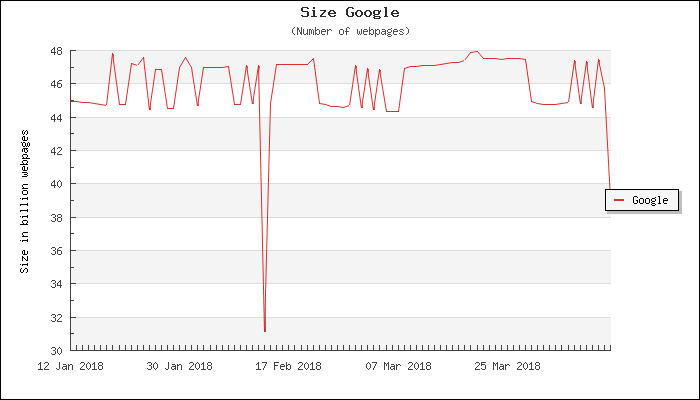
\includegraphics[width=.8\textwidth]{img/google_webpages.png}
\caption{The amount of webpages indexed by Google}
\label{fig:graph_googleweb}
\end{figure}
Google proved to be the most used web search engine by processesing the vast majority of all the web search queries. It held 81.53\% of the search engines market share from January 2017 to January 2018, as shown in \autoref{fig:graph_market}\footnote{provided by \texttt{netmarket.com}}.
\begin{figure}
\centering
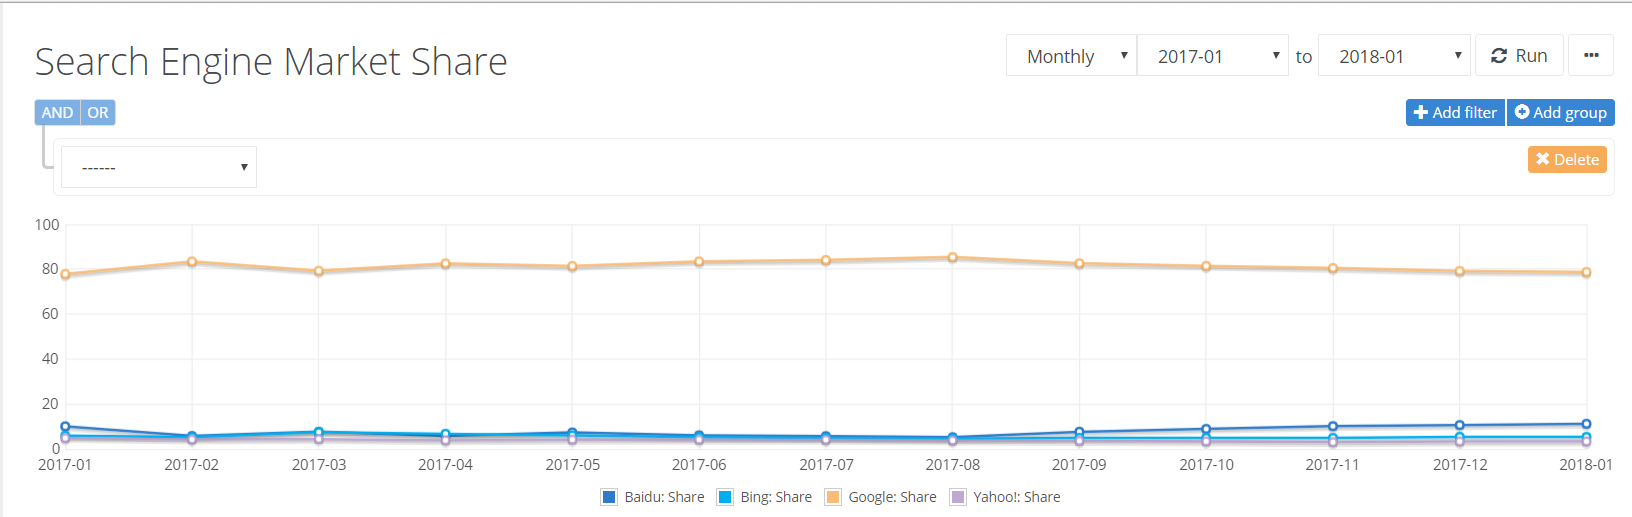
\includegraphics[width=.8\textwidth]{img/search_engine_market.png}
\caption{The search engine market on all platforms in 2017.}
\label{fig:graph_market}
\end{figure}

Complementary to the already mentioned automated search engines relying on keyword matching, there exist human maintained search engines. They may return more sufficient answers but are expensive to build and hard to maintain~\cite{google}.

The collections used by the search engines can be vastly distinct from each other: For example, they can vary in size. Some collections can be as small as tens of megabytes and grow each day by only few hundreds of documents. Others may contain tens of gigabytes (e.g. libraries) but still grow slowly. Web collections are different, they are not only extremely huge, but the amount of indexed data can change drastically both ways. Google has currently around 40 billion documents indexed. However, on the 17th of February, they had indexed only around 31 billions of documents.

The search engine we found to be the most attractive option for KamehaMail is ElasticSearch. As we covered the topic of text search and the search engines, we can look into its specifications.

\subsection{ElasticSearch}
\label{es}
In this part, we detail the specific implementation parts of the ElasticSearch because we integrated it into KamehaMail for the role of search-engine database. All the facts and information are interpreted from the book written by Gormley and Tong~\cite{elastic}.
ElasticSearch is very popular open-source analytics and search engine built on top of Apache Lucene, which is a full-text search library, used by corporations such as Wikipedia or Github. ElasticSearch runs on its own server communicating via provided RESTful API and JSON.

In the following paragraphs, we cover most of the implementation problems that we faced earlier in this chapter and look at the solutions ElasticSearch provides.

\subsubsection{Document Metadata}
ElasticSearch has three mandatory meta data fields stored along with the document. \emph{Index} is a document collection where the document is stored. \emph{Type} is a subcategory of the index. It defines specific mappings to the documents of the same type. This mapping is stored with the type and the queries performed against it are analyzed the same way. It is possible to have several types in the same index.
The last field is \emph{id} which is a string that along with the index and type uniquely identifies the document.

\subsubsection{Structure}
ElasticSearch uses a specific terminology for its structures. The main part of whole system is a \emph{cluster}. A \emph{Cluster} is a collection of servers that are capable of indexing, searching and holding all the data. These servers are called \emph{nodes}. It is possible to run multiple nodes in a single cluster. An image of empty initialized cluster is shown in \autoref{fig:empty-cluster}. It is a one node cluster, called \texttt{master}.
\begin{figure}
\centering
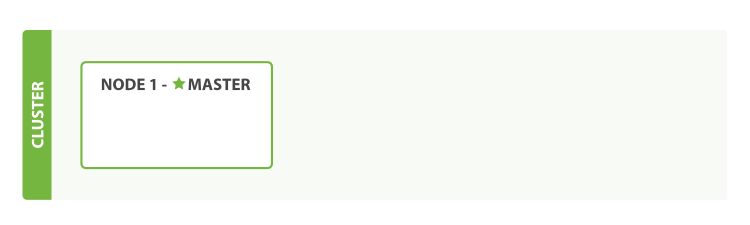
\includegraphics[width=.8\textwidth]{img/empty_cluster.png}
\caption{An empty cluster.}
\label{fig:empty-cluster}
\end{figure}

We would like to remind the problem of large amount of the data in an index mentioned in \autoref{index}. ElasticSearch solves this by splitting the index into the user-defined amount of \emph{shards}. \emph{Shard} is an independent and fully-functional index, capable of searching and indexing by its own.
The usage of shards is fully transparent to the user. In addition, ElasticSearch provides a possibility of creating copies of the shards, called \emph{replicas}. \emph{Replicas} are 1:1 clones of shards, used to ensure high availability of the indexed data. If new data is inserted into the primary shard, it is copied to its replica as well.
The replicas are also used to speed up the search by working concurrently with the shards.
An example of simple commonly used cluster is shown in \autoref{fig:replicas} that contains three shards and one replica for each shard.
\begin{figure}
\centering
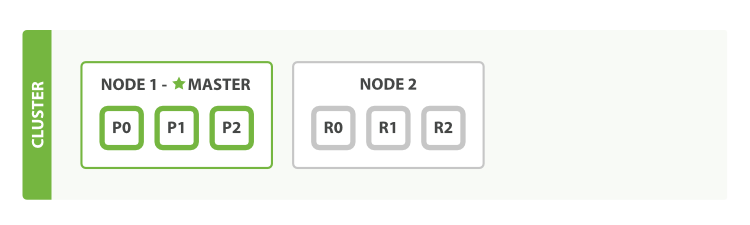
\includegraphics[width=.8\textwidth]{img/replicas.png}
\caption{A cluster with one node Master that is subdivided into three shards P0, P1 and P2. In the node 2, there is one replica shard (R0, R1, R2) for each primary shard.}
\label{fig:replicas}
\end{figure}

\subsubsection{Result score}
ElasticSearch uses \emph{Lucene's practical scoring function}~\cite{elastic} for ranking the matches.
The formula is as follows:
\begin{align*}
\centering
\textrm{s}(q,d) = \textrm{nq}(q) \cdot \textrm{c}(q,d) \cdot \sum_{t \in q}\textrm{f}(t,d) \cdot \textrm{if}(t)^2 \cdot\textrm{b}(t) \cdot \textrm{nt}(t,d),
\end{align*}
where
\begin{itemize}
\item $s(q,d)$ is the final relevance score of the query $q$ in the document $d$,
\item $\textrm{nq}(q)$ is the query normalization factor, it is used for normalizing the query $q$ in order to be able to compare it to the others,
\item $\textrm{c}(q,d)$ is the coordination factor, used to add additional score to the documents that contain higher percentage of the query terms,
\item $\textrm{f}(t,d)$ is the frequency of the term $t$ in the document $d$,
\item $\textrm{if}(t)$ is the frequency of the term $t$ in the inverted index,
\item $\textrm{b}(t)$ is a boost to the term $t$ for the query $q$, and
\item $\textrm{nt}(t,d)$ is the field-length normalization. The shorter the field, the higher the weight.
\end{itemize}

We believe that ElasticSearch is a great choice for performing the full-text search in the database of indexed e-mails as it is provides strong performance and simple interface.

\section{Application to mail indexing}
Short response time for searching in e-mails is necessary for modern e-mail user interface. 
To provide this feature, we parse the information from an e-mail message and index it into the respective fields of ElasticSearch's index. The analyzed fields are \texttt{subject}, \texttt{text}, \texttt{to} and \texttt{from}. Non-analyzed fields are \texttt{messageid}, \texttt{references} and \texttt{tag} as we want an exact match and not similarity match. The last used field is \texttt{date} which is not only analyzed but also mapped (by standard date formats) because we want the results to be sorted primarily by the date and then ranked by the relevance.

Not only user-defined searches but also many other functions are handled by ElasticSearch. Grouping of the emails by references is done by ElasticSearch. As the e-mail directory-based hierarchy is replaced by tags, these are searched by ElasticSearch as well.

\chapter{Implementation}
\label{implementation}
In this chapter, we show an overview of all the implementation tools and procedures that we used to create KamehaMail. The implementation is separated into two major parts: the backend which communicates with the mailserver and the search engine, and the browser-based frontend that provides an interface to the end-user. These two parts communicate with each other using API calls.

\section{Backend}
 The implementation of the backend follows the usual style of deployment of PHP application. The software on the server is organized as follows:
\begin{itemize}
\item \emph{Apache HTTP server} is used to serve the static frontend files and the end-user's web browser, and provides the translation of the browser-originated HTTP API calls to the PHP application.
\item The application is run by \emph{PHP} with several additional modules (the complete list is shown in \autoref{userguide}).
\item The application communicates with \emph{Exim4} mail server using standard UNIX methods: \texttt{sendmail} for sending e-mail and pipe-based transport for receiving. Exim handles the communication with the e-mail infrastructure using standard internet protocols. It is also possible to integrate other mail servers.
\item \emph{ElasticSearch} is installed for searching and indexing the e-mails. The server communicates with it via REST API using \texttt{curl} requests.
\end{itemize}

\subsection{Data storage}
The data on the server are stored on two different places: the primary storage of the e-mails as files in user directories, and the secondary indexed storage in ElasticSearch.

The primary storage is organized as follows: in a specified directory 
the application stores the meta-information about users
(e.g. login details) and the users' mailboxes.

The mailbox section contains all the stored e-mails. Each e-mail is uniquely identified by its 64-character Sha-256 hash. The e-mails are separated into users' subdirectories, in which they are further separated into a subdirectory structure based on first few characters of the hash, to minimize the problems with large directories.

The meta-information section contains two SQLite databases, \texttt{usersdb} and \texttt{loginkeys}. \texttt{usersdb} is a list of all users and their corresponding passwords. \texttt{loginkeys} is a list of the currently logged users and their corresponding login API keys (further explained in \autoref{userapi}).

The directory hierarchy is displayed in \autoref{fig:folder-tree}.
 \begin{figure}
\centering
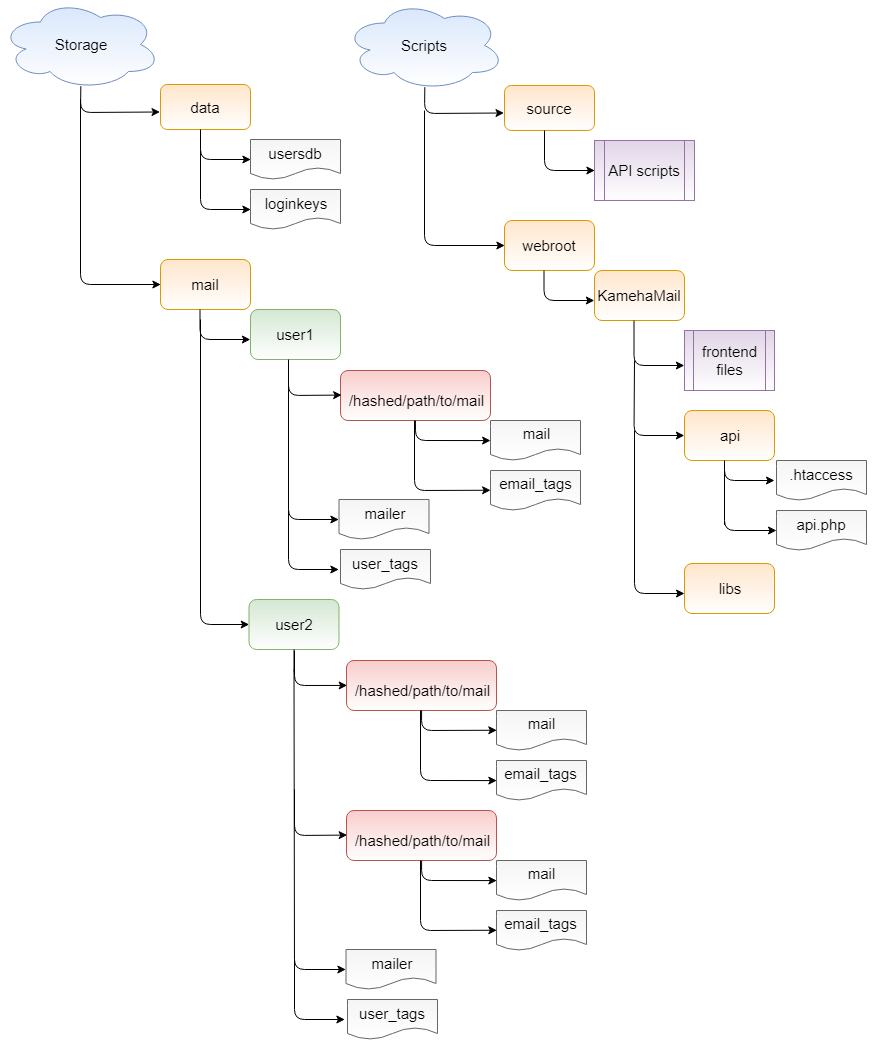
\includegraphics[width=\textwidth]{img/folder_tree.png}
\caption{A folder hierarchy on the server}
\label{fig:folder-tree}
\end{figure}

\subsection{API}
All of the server side scripting was done in PHP. To simplify the communication between the frontend and the backend, we created a set of API calls which run specific PHP scripts.

To provide REST-like API calls, htaccess is used. If an HTTP request is directed to the folder where the \texttt{.htaccess} is located, \texttt{htaccess} takes the request's URL and forwards it as a query string to a beforehand defined script. For example, upon calling URL
\begin{center}
\texttt{hruska.blesmrt.cf/KamehaMail/api/some-work}
\end{center}
htaccess takes a part of the url after its folder's name (i.e. \texttt{some-work}) and sends it to the \texttt{api.php} as a query string. \texttt{api.php} serves as a relay or a router. It loads all necessary source scripts and calls other PHP scripts accordingly to the received query string.

We provide an example of the processing of the user login API request:
\begin{enumerate}
\item  A HTTP POST request is sent from the frontend to the URL\\\texttt{api/client/login} with the data: \texttt{username} and \texttt{password}.
\item \texttt{.htaccess} in the api folder processes the url string and redirects\\\texttt{client/login} as a query string to the \texttt{api.php}.
\item \texttt{api.php} parses the query string, calls an external \texttt{login} function (defined by \texttt{login.php} in the source folder) with the username and password as parametres.
\item The login function checks the credentials and returns a JSON formatted response whether the login was successful or not, together with a new API key (which is simultaneously stored to the \texttt{loginkeys} database).
\item Then \texttt{api.php} forwards the response to the frontend.
\end{enumerate}

The source folder contains many of the PHP scripts for different uses. In the \autoref{fig:folder-tree}, they are denoted as \texttt{API scripts}. Depending on their purpose, they can be divided into three categories:

\subsubsection{Client calls}
\emph{Client} scripts are used for the account management such as logging or changing passwords.
\begin{itemize}
\item \texttt{login.php} validates the given credentials. In case of success, it creates a loginkey (hash of the current time, username and password), saves it to the \texttt{loginkeys} database and sends it to the frontend which saves it to the browser as well (similar to cache). This loginkey is later used to validate the API calls.
\item \texttt{checklogged.php} checks whether the currently saved loginkey is valid. If yes, logged user is redirected to his e-mails page.
\item \texttt{logout.php} removes the currently used loginkey from the database and redirects the user to the homepage.
\item \texttt{mailer.php} contains functions for setting/getting the mailer of the user.
\item \texttt{password.php} changes the password of the user.
\item \texttt{signup.php} creates new user entry in the \texttt{usersdb} database and a new folder in mail. It also initializes new index in the ElasticSearch with the user's name and the e-mail mapping.
\item \texttt{usertags.php} contains functions for adjusting the user's tags. Each user can have self-defined tags which are stored in their mail folder.
\label{userapi}
\end{itemize}

\subsubsection{Integration of the ElasticSearch to the server}
\emph{Elastic} scripts communicate with the ElasticSearch via provided RESTful API. We implemented it to the API scripts using PHP curl requests.  
The following code is an example of a PHP \texttt{curl} request which calls Elastic's search API.
\pagebreak
\begin{code}
$req = curl_init();
    
curl_setopt_array($req, [
    CURLOPT_URL            =>
	 "http://localhost:9200/user/email/_search?pretty",
    CURLOPT_CUSTOMREQUEST  => "GET",
    CURLOPT_POSTFIELDS     => $data,
    CURLOPT_HTTPHEADER     => [ "Content-Type: application/json" ],
    CURLOPT_RETURNTRANSFER => true,
]);
    
$response = json_decode(curl_exec($req));	
$curl_close($req);
\end{code}
\texttt{\$req} is an initialized \texttt{curl} request. \texttt{CURLOPT\_URL} ultimately contains the API call. The call is directed to the localhost:9200\footnote{ElasticSearch listens to this port} with index \texttt{user}, type \texttt{email} and the function \texttt{\_search}. \texttt{\$data} contains the query in a JSON format. The response is sent as a JSON string back from ElasticSearch and saved in \texttt{\$response}.
We implemented following scripts which use ElasticSearch:
\begin{itemize}
\item \texttt{search.php} processes user's query and reformats it to the ElasticSearch's syntax. After being processed by ElasticSearch, the results of the search are sorted by the \texttt{date} field. \texttt{search.php} in fact runs two searches. The first search finds e-mails relevant to the given query and returns their identifiers. Second search creates so-called mail groups:  The e-mails are grouped by references to create a conversation-like interface. ElasticSearch's search is called for each matched document, matching also the documents which have the already found identifier in their references. This will result in a list of grouped e-mail identifiers where in each group at least one of the e-mails was a result of the former user's query.
\item \texttt{updatetags.php} changes tags in ElasticSearch for the specific e-mail.
\item \texttt{removeMail.php} removes the e-mail from ElasticSearch.
\item \texttt{saveMail.php} puts new e-mail document to the ElasticSearch. If the inserted e-mail has some references (to already present e-mails), each of the referenced e-mail messages is updated with its \texttt{message-id}.
\item \texttt{reindex.php} takes hashes of already stored e-mail in the database and gives their parsed content to ElasticSearch for reindexing.
\end{itemize}
 
\subsubsection{Communication with e-mail server and processing of e-mails}
\emph{E-mail} scripts implement the handling of e-mails:
\begin{itemize}
\item \texttt{maildrop.php} is called when the mail server receives new message. It retrieves its content and forwards it to the \texttt{decide} function (defined by \texttt{decide.php}).
\item \texttt{decide.php} is the actual brain behind storing the messages. It checks whether the recipient is a legit address, parses the contents of the message, creates tags, stores it to the mail directory and forwards the parsed data to the saving function of ElasticSearch.
\item \texttt{downloadAtt.php} temporarily saves the received attachment to the server and forces the browser to download it. Then removes the attachment.
\item \texttt{getMail.php} receives resulting IDs from Elastic's \texttt{search} function and processes them. It finds the corresponding e-mail files in the mail directory, parses them and sends their contents to the frontend which displays them. It also takes care of the date separation of the e-mails.
\item \texttt{changetags.php} changes user's tags.
\item \texttt{removeAtts.php} contains function which is called whenever the upload of the attachments was cancelled or the e-mail was sent, to remove them from the server.
\item \texttt{removeMail.php} removes the e-mail from the mail directory.
\item \texttt{saveMail.php} saves the e-mail to the mail directory.
\item \texttt{sendMail.php} creates headers for sending an e-mail and sends it.
\item \texttt{upload.php} temporarily uploads the attachments to the server, for future sending.
\end{itemize}
We used two external libraries to simplify the processing of e-mail text: \emph{mailparser}\footnote{\texttt{https://github.com/php-mime-mail-parser/php-mime-mail-parser}}, which extracts headers, bodies and attachements from an e-mail, and \emph{PHPMailer}\footnote{\texttt{https://github.com/PHPMailer/PHPMailer}}, which creates all necessary headers for sending a message and actually sends it.

The source folder also contains an administration interface, which is accessible using \texttt{admin.php}. The usage of admin interface is further described in \autoref{userguide}.

\section{Frontend}
Frontend provides the interactive visual side that come to contact with the user. The frontend is coded in JavaScript, HTML and CSS.

\paragraph{Choice of JavaScript framework.}
Framework is a software structure that provides functionality for building specific applications. Some of the most favourite JavaScript frameworks are Vue, Angular, React or Ember. We chose \emph{Vue}\footnote{https://vuejs.org/} for KamehaMail because it is fast, scales well and has a simple API to use.
Its core part is a Vue instance which configures the application, binds the data and attaches the application to a specific DOM element. Another important thing is that there exists a component framework for Vue, called \emph{Vuetify}\footnote{https://vuetifyjs.com/en/}. It is a UI toolkit, providing many templates that are directly cooperating with Vue.
We used several of these templates to make KamehaMail pleasant to look at.

\paragraph{Frontend application structure.}
The frontend is divided into three important parts. Each of them consists of an HTML file and a JavaScript file. The first part is \texttt{index}, which is the first thing an user will encounter upon opening the main site. It is a simple login menu with an option to sign up. On successful login, user is redirected to the main menu where he can see his e-mails.
The second part is \texttt{signup} which is visually very similar to the \texttt{index}. The third and the biggest part is \texttt{emails} which implements all of the interface's features.
For the message text editor we integrated \emph{quill}\footnote{consists of two parts, official quill from \texttt{https://quilljs.com/} and the Vue implementation for it taken from \texttt{https://github.com/surmon-china/vue-quill-editor}}.All used libraries, such as Vue, Vuetify and jQuery are stored along with their CSS files in the folder \texttt{libs} in KamehaMail, to be accessible to the frontend.

\subsection{Communication with the server}
The frontend and the backend communicate with each other via asynchronous POST HTTP requests sent from the frontend to the server. The frontend uses the jQuery's feature \texttt{ajax}, which takes care of sending the requests and receiving the responses from them in a user-friendly way.

\chapter{Results}
\label{results}
In this chapter, we investigate the performance of the resulting software.

KamehaMail is fully functional and implements almost all of the intended features. Additionally, we test the scalability of the searching capabilities of the interface on large amount of e-mails.

\section{Benchmark setup}
First of all, we prepared an environment sufficient for testing. Enron e-mail data set\cite{klimt2004enron} is a collection of roughly half million e-mails, freely accessible for anyone. Using the implemented admin interface, we dropped and indexed the Enron e-mails into one mailbox in the database. The e-mails were tagged according to the original position in the folder.

We measured the results on two data sets of different sizes to provide better overview of performance scaling.

The first data set consists of almost 27.000 e-mails found in the mailbox of the Enron user V. Kaminski. The second data set consists of 200.000 e-mails selected randomly from multiple mailboxes. The full data set was not benchmarked because of resource limitations.

On both data sets, we measured the space needed for their storing in the database, and the time required to complete several testing queries.

\section{Benchmark results}
The results obtained on the indexed data sets are reported in \autoref{table:bench}.

As expected, the more complicated cases were tested, the longer it took ElasticSearch to give the results. Increases in response time were caused by more complex queries, more indexed e-mails and more returned results. On the other hand, from the perspective of the user, the 7.4-times increase in the amount of data did not have a significant impact on the response time of the search. 

The indexing process itself scaled satisfactorily --- indexing performance was approximately 40 e-mails per second on average, and it varied only negligibly with the increase of the index e-mail count.
\begin{table}[t]
\centering
\renewcommand{\arraystretch}{1.4}
\begin{tabular}{p{10em} l l}
 \toprule
Query & 26.675 e-mails & 200.000 e-mails\\
\midrule
\texttt{tag:inbox} & &\\
\hline
Top 10 results & 1ms & 5ms\\
Top 50 results & 3ms & 8ms\\
Top 100 results & 8ms & 11ms\\
\hline
\texttt{tag:inbox and approval}  & &\\
\hline
Top 10 results & 14ms & 48ms\\
Top 50 results & 16ms & 68ms\\
Top 100 results & -- & 70ms\\
\hline
\texttt{tag:inbox and approval and time:<1.1.2002}  & &\\
\hline
Top 10 results & 18ms & 52ms\\
Top 50 results & 20ms & 59ms\\
Top 100 results & -- & 57ms\\
\hline
 & &\\
\hline
E-mail files disk space & 417MB & 2.7GB\\
ElasticSearch's index disk space & 112MB & 394MB\\
\bottomrule
\end{tabular}
\caption{Search and space results from benchmark performed on Enron e-mail data set.}
\label{table:bench}
\end{table}

\chapter*{Conclusion}
\addcontentsline{toc}{chapter}{Conclusion}
This thesis has reviewed the necessary means and tools for creating a modern, web-based end-user e-mail interface, mainly the high-performance full-text search and customisable tags, while avoiding the usage of mail folders for mail organization. The main result of the thesis, the mail interface KamehaMail, provides a simple open-source alternative to the commercial user interfaces (e.g. Google Inbox).

In \autoref{mailprocess} we have discussed the format of e-mail messages, e-mail exchange on the Internet and several details of the related e-mail infrastructure; including the classification of mail-transfer agents and brief description of the used communication protocols. We reviewed and classified some of the existing end-user e-mail interfaces, which are the main concern of this thesis.

In \autoref{textsearch}, we have described the currently used techniques for creating a working searchable database using an inverted index structures, which can be later used for implementing a database capable of high-performance. We have provided several examples of used queries and of the matching process. At the end, the chapter compares the full-text search to standard database search and looks briefly at the current search engines.

Finally we have connected an open-source search engine ElasticSearch to the mail processing infrastructure and a web-based end-user interface to create KamehaMail. Implementation details, used tools, frameworks and libraries are detailed in \autoref{implementation}. 

We have benchmarked KamehaMail (and ElasticSearch) by indexing approximately 200 thousand e-mails from the publicly available Enron e-mail data set~\cite{klimt2004enron} and measuring the search time required to complete several queries in the resulting mailbox. The results are available in \autoref{results}.

KamehaMail can run on any reasonably modern UNIX-like operating system that can run a mail server, a web server, and ElasticSearch. A simple installation and user guide is provided in \autoref{userguide}.

\section{Future work}
The implementation of KamehaMail is not perfect and we provide ideas for the improvement of both interface and the API library:
\begin{itemize}
\item Implement safety measures against JavaScript e-mail messages.
\item Support for more complex queries. The search possibilities of the current interface are limited due to the desired simplicity of the user queries. ElasticSearch offers great variety of different options for querying, which can be mapped to the syntax of KamehaMail queries to expose more functionality to the users.
\item Implementation of built-in calendar and a snooze feature (known from Google Inbox) would benefit the connection of user e-mail management to time-management. KamehaMail API can be easily extended to support this feature.
\item Hierarchical tags are a feature that can provide the hierarchical mail-classification workflow of nested directory structures while still providing the ability to search by tags without the cumbersome parallel maintenance of both classification structures. ElasticSearch supports this kind of tagging via wildcard queries.
\item Addition of more user account management possibilities, e.g. avatars, signatures, mail aliases, addressbooks, or other commonly expectable features.
\item Improve the design of the interface to work nicely on smartphones (or generally smaller screens), or create a native mobile application that communicates directly with the KamehaMail API.
\item Caching of the search results to the browser for speeding the interface's response time.
\end{itemize} 

%%% Bibliography
%%% Bibliography (literature used as a source)
%%%
%%% We employ bibTeX to construct the bibliography. It processes
%%% citations in the text (e.g., the \cite{...} macro) and looks up
%%% relevant entries in the bibliography.bib file.
%%%
%%% The \bibliographystyle command selects, which style will be used
%%% for references from the text. The argument in curly brackets is
%%% the name of the corresponding style file (*.bst). Both styles
%%% mentioned in this template are included in LaTeX distributions.

\bibliographystyle{alpha}    %% Author (year)
% \bibliographystyle{unsrt}     %% [number]

\renewcommand{\bibname}{Bibliography}

%%% Generate the bibliography. Beware that if you cited no works,
%%% the empty list will be omitted completely.

\bibliography{refs}

%%% If case you prefer to write the bibliography manually (without bibTeX),
%%% you can use the following. Please follow the ISO 690 standard and
%%% citation conventions of your field of research.

% \begin{thebibliography}{99}
%
% \bibitem{lamport94}
%   {\sc Lamport,} Leslie.
%   \emph{\LaTeX: A Document Preparation System}.
%   2nd edition.
%   Massachusetts: Addison Wesley, 1994.
%   ISBN 0-201-52983-1.
%
% \end{thebibliography}


\appendix
\chapter{User Guide}
\label{userguide}
In this appendix, we provide a user guide for running the interface on own infrastructure or simply using it for e-mail management.

The appendix is separated into two sections. The first section describes the interaction with the interface on the end user's level. The second section details the API library, and explains how to run the interface on a UNIX server.

\section{Interface interaction}
KamehaMail can be tried on the webpage \texttt{hruska.blesmrt.cf/KamehaMail} using any reasonable modern web browser. The main page is a simple login panel with sign up option. To registrate, go to the \texttt{Sign Up} option, choose a username (with domain at the end, in this case \texttt{@hruska.blesmrt.cf}).

After successful login, the e-mails page shows up. There are several points of interest:

\paragraph{Left navigation panel.}
Left navigation panel contains tags for e-mails. First four tags are system tags, \texttt{Inbox}, \texttt{Archive}, \texttt{Trash} and \texttt{Sent}. After them comes menu with customisable user-defined tags\footnote{list of possible icons for tags can be found on \texttt{https://material.io/tools/icons/}}. There is a possibility to create a search tag from the current search.

\paragraph{Top bar.}
The top bar contains search panel (center) and account management menu (right). Possible queries for the search are the following:
\begin{itemize}
\item User can simply type the term he is searching for. In this case, the search engine will look into all analyzed fields for the match.
\item User can specify the search field, for example \texttt{subject: Hello}. Possible search fields are \texttt{subject}, \texttt{text}, \texttt{from} and \texttt{to}
\item There is one more unanalyzed search field named \texttt{tag}. Any system or user-defined tags can be searched using the same syntax (e.g \texttt{tag: inbox}).
\item User can filter the results by date. Date value must be in \texttt{time: dd/mm/yyyy} or \texttt{time: dd.mm.yyyy} format. Possibilities of date filtering are:
\begin{itemize}
\item lesser than \texttt{time: <date}
\item greater than \texttt{time: >date}
\item between \texttt{time: date-date}
\item exact date \texttt{time: date}.
\end{itemize}
\end{itemize}
All of the queries above can be combined using \texttt{and}, creating multi-criteria queries with any number of white spaces in between.
Account management provides options for password change, mailer change and logout.

\paragraph{Center.}
The button in the bottom right corner opens a form for writing a new e-mail. It features text editor and a file drop for attachments.

The center contains grouped e-mails. Each group indicates the number of the e-mails it references to and the subject of the conversation. If the subject is in bold, one or more messages in the conversation are new (i.e. unread). The tag buttons are to the right of the subject: mark read/unread, archive, delete and a drop-down menu for user's tags.
Preview of each e-mail is shown once the group is opened. Each e-mail group provides text editor and \texttt{Quick Reply} option to reply directly to the conversation. Reply and forward options on the right side of each e-mail open a new prefilled form for sending.

All basic features are displayed in \autoref{fig:menu}.
\begin{figure}
\centering
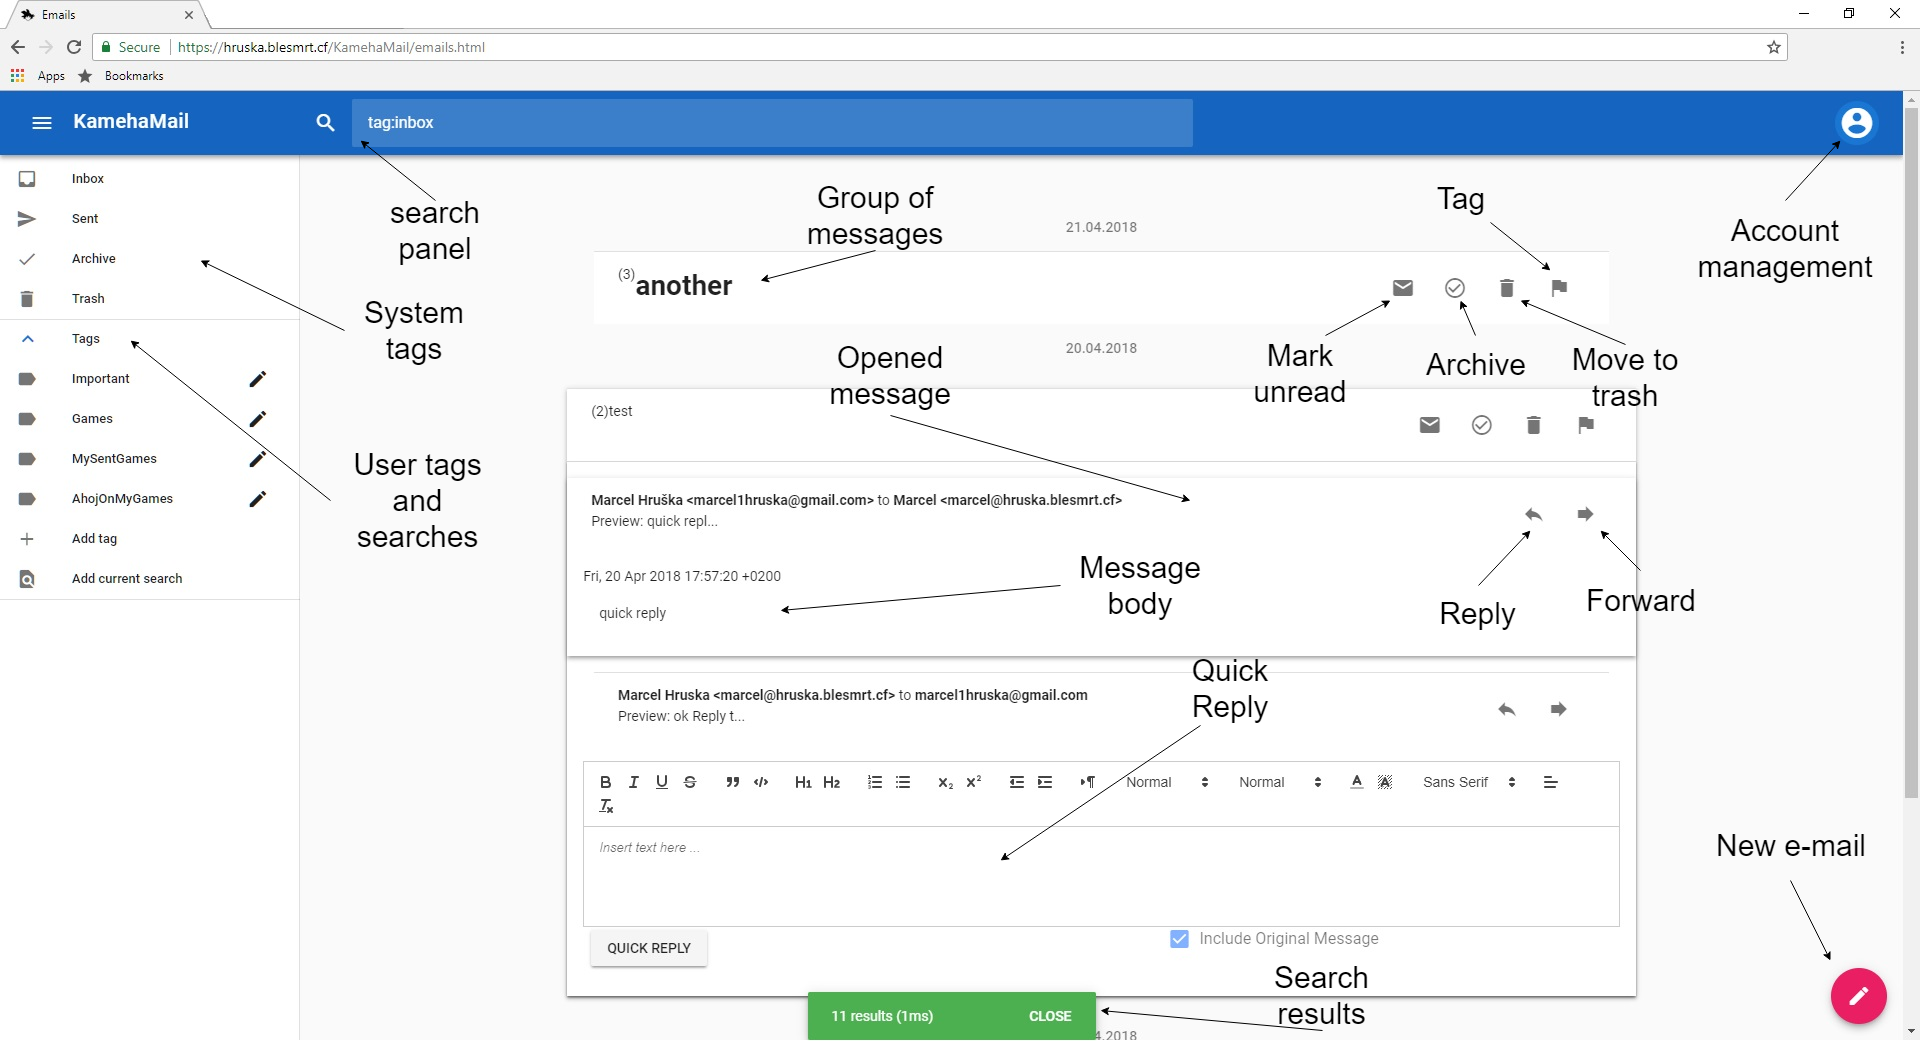
\includegraphics[width=\textwidth]{img/menu.png}
\caption{Main menu description.}
\label{fig:menu}
\end{figure}

\section{Server configuration}

We briefly cover the installation procedure for getting KamehaMail working on a UNIX server. The requirements are:
\begin{itemize}
\item A running ElasticSearch cluster accessible on \texttt{localhost} port 9200.
\item A web server (Apache is preferred because of the \texttt{.htaccess} usage, but any webserver capable of request rewriting will work). Apache module \texttt{mod\_rewrite} is required; \texttt{mod\_ssl} is highly recommended since KamehaMail does not do any encryption of data on its own. Using \texttt{mod\_suexec} for executing the API is also recommended for additonal security.
\item A working mail server (we use Exim4 as an example, but any server that can route local mail delivery to a program pipe will work, including Postfix, Sendmail, Courier and other).
\item PHP interpreter, preferably of version 7 or better, with following modules available:
\begin{itemize}
\item php-curl
\item php-gd
\item php-json
\item php-mail
\item php-mailparse
\item php-mbstring
\item php-net-smtp
\item php-net-socket
\item php-pear
\item php-sqlite3
\item php-xml
\end{itemize}
\end{itemize}



For the installation, KamehaMail backend is extracted on the server. The source code can be currently obtained from the Git repository at \url{https://github.com/hrusticka123/KamehaMail}.

The configuration consists of creating a storage space for the primary e-mail database, configuring Apache webserver and setting up the local mail transport to KamehaMail.

\begin{enumerate}
\item Paths to mailbox directory, data directory (as described in \autoref{implementation}) are filled into \texttt{source/config.php}, together with the full absolute path to the \texttt{source} directory. KamehaMail script should have write access to the mailbox and data directory. \texttt{/var/lib/kamehamail} is a preferable location for both.
\item The extracted directory contains a subdirectory \texttt{webroot}, which is where Apache document root should be directed. Webroot contains a subdirectory \texttt{api} with files \texttt{.htaccess} and \texttt{api.php}, which serve as a gateway to the rest of the implementation. Apache must be configured to execute \texttt{api.php} as a CGI script (possibly by FastCGI, FCGID or php-fpm).
\item Path to the \texttt{source} directory must be filled in \texttt{api.php} so that it can find the rest of the backend source code.
\item To allow mail exchange, the UNIX user that runs KamehaMail source code must have access to \texttt{sendmail} command.
\item Receiving mail from the mail server is implemented by piping the incoming e-mail to the script \texttt{maildrop.sh}, which forwards it to the PHP application. Configuration of Exim4 for this behavior consists of several steps that modify the Exim4 configuration:
\begin{enumerate}
\item The mail domains that are handled by KamehaMail instance are put into the list \texttt{dc\_other\_hostnames}, which effectively makes them `local domains' for Exim.
\item The local user transport is changed to\\ \texttt{transport = transport\_kamehamail}.
\item A corresponding transport configuration is created in the directory with mail transports:
\begin{code}
transport_kamehamail:
	driver = pipe
	command = /var/www/example.org/maildrop.sh
	user = kamehamail-user
	group = kamehamail-group
\end{code}
(Path to \texttt{maildrop.sh}, user and group should be changed to match local setup.)
\end{enumerate}
Other mail servers can be set up for similar behavior.
\end{enumerate}

After setting up and reloading all services, KamehaMail should be ready to register new users and accept e-mail.

Extra interface is provided for the usual administrative commands: script \texttt{source/admin.php} can be run with \texttt{php} to execute administrative tasks, such as user management, reindexing or e-mail injection. The list of commands is available in \autoref{table:admin-calls}. For example, a new user is added by running:\\
\texttt{php api.php add\_user john.doe@example.com johnspassword} \\
The same interface was used during benchmarking to easily index the dataset and make it available to the web interface for measurements.
\begin{table}[t]
\centering
\renewcommand{\arraystretch}{1.4}
\begin{tabular}{p{6em} l l p{6em}}
 \toprule
Description & Command & Parameters & Script standard input \\
\midrule
Inject \mbox{an e-mail} & \texttt{drop} & \texttt{user@domain tag} & RFC-formatted content of e-mail\\
Reindex mail &  \texttt{reindex} & \texttt{user@domain} & list of hashes to reindex\\
Add user & \texttt{add\_user} & \texttt{user@domain password} & -- \\
Remove user & \texttt{remove\_user} & \texttt{user@domain} & -- \\
Remove \mbox{a specific} mail & \texttt{remove\_mail} & \texttt{user@domain} & list of hashes to remove\\
\bottomrule
\end{tabular}
\caption{Administration interface command listing.}
\label{table:admin-calls}
\end{table}


\openright
\end{document}
